\chapter{Hambledon Hill} %17,300
\label{ch:hambledon}
This chapter considers the temporal and spatial evidence of Hambledon Hill, it will undertake a detailed review of the temporal data, analysing the distribution of that data across the site. The review will focus on how the evidence supports the interpretations of \citet{Mercer:2008fk} and  \citet{Whittle:2011kl} and whether combining the spatial evidence enhances or damages the confidence in those interpretations, potentially opening up the door to re-evaluate the evidence. Following this, the spatial evidence will be re-combined with the temporal in a series of analysis that re-contextualises the temporal evidence in it's spatial context. This analysis will demonstrate the benefits that can be gained by such combined analysis and will provide new insights into the nature of the available data set at Hambledon. Following this, there will be a review of the interpretation offered by the original investigation, drawing on the new evidence to perform a critical evaluation, crucially enabling an identification of the limitations with the available data. The fundamental purpose of the study is to evaluate how the existing interpretation is supported by the temporal evidence, compare this to how well the same interpretation is supported by the spatio-temporal evidence and investigate any areas where the interpretation can be enhanced.

\section{Background}

\begin{figure}
\begin{center}
	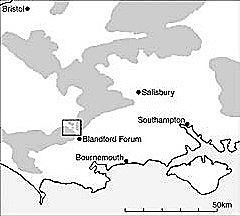
\includegraphics[width=0.7\textwidth]{figures/hambledon-location}
\end{center}
  \caption{Location of Hambledon Hill, from \citep[2]{Mercer:2008fk}}
  \label{fig:location}
\end{figure}

Hambledon Hill is a site of intense prehistoric activity, including two causewayed enclosures, two long barrows, neolithic defensive earthworks, \citep[xiii]{Mercer:2008fk} potentially as many as six round barrows \citep[12]{Mercer:2008fk} a hillfort and field systems. The site is situated in Dorset, South West England on the southern edge of Cranborne Chase. Between 1974 and 1986 Roger Mercer directed a programme of excavation the result of which is the published volume, \citet{Mercer:2008fk}. This was made up of nine seasons of large scale excavations, followed by more targeted investigations in the Everley Water Meadows in 1983 and 1984 and the hillfort in 1986 \citep[11]{Mercer:2008fk}. Figure~\ref{fig:excavations} shows the site, its key features and the main excavated areas. The interpretations offered are detailed and cover a broad range of topics, from a temporal perspective, they cover how the site developed over time, reproduced in figure~\ref{fig:hambledon-devel}. The interpretations of \citep{Whittle:2011kl} are more than just a linear progression of the site's features, they also offer probable lengths of time that each phase would have taken and duration of the gaps between phases. This interpretation is punctuated by key chronological events, such as the burial of individuals and the conflict surrounding the burning of the Stepleton Outwork. In addition it places the infilling and associated abandonment of areas of the site in their chronological context, showing how the focus of activity (or activities) shifted around the site over time. 

\begin{figure}
\begin{center}
	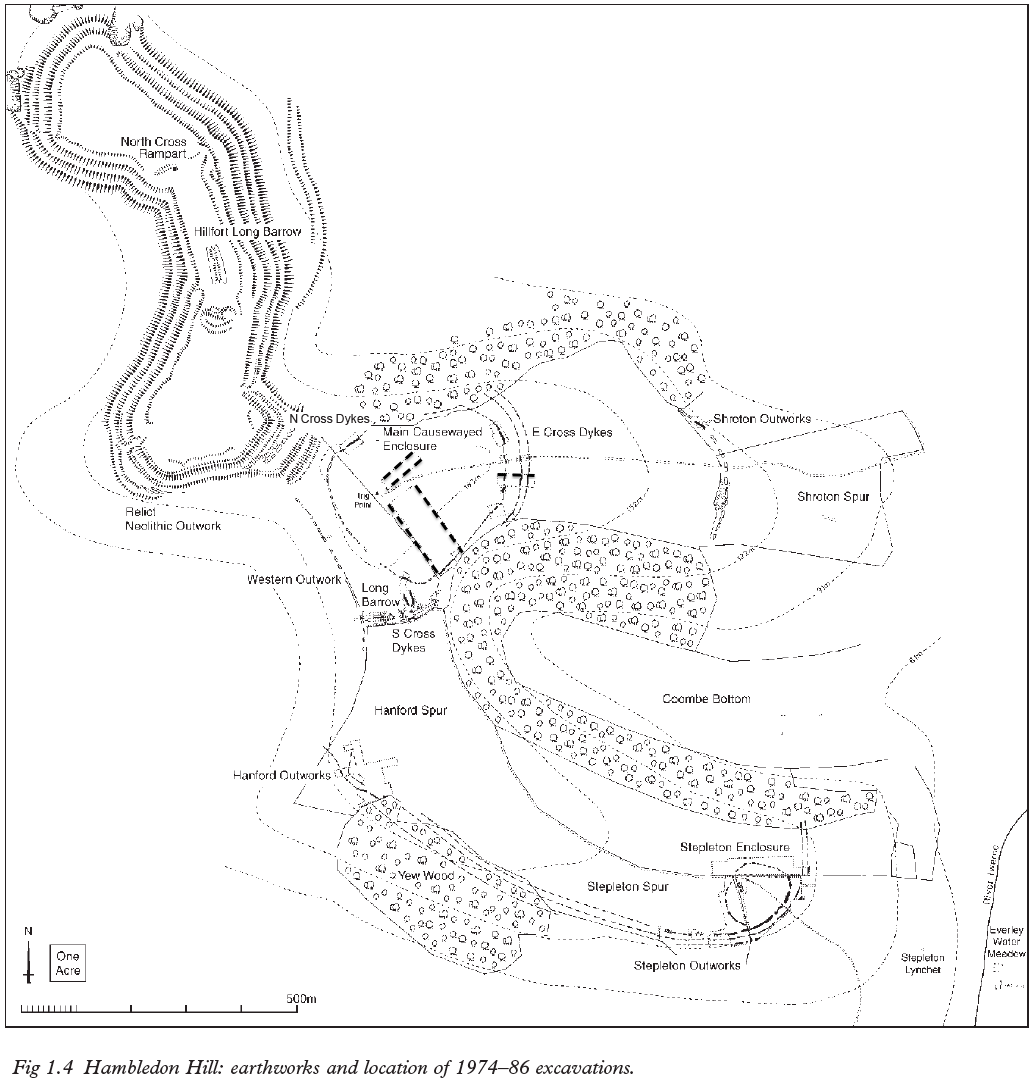
\includegraphics[width=0.9\textwidth]{figures/excavation-plan}
\end{center}
  \caption{Plan of main earthworks and locations on Hambledon Hill, from \citep[5]{Mercer:2008fk}}
  \label{fig:excavations}
\end{figure}

\section{The Temporal Evidence}

\begin{figure}
\begin{center}
	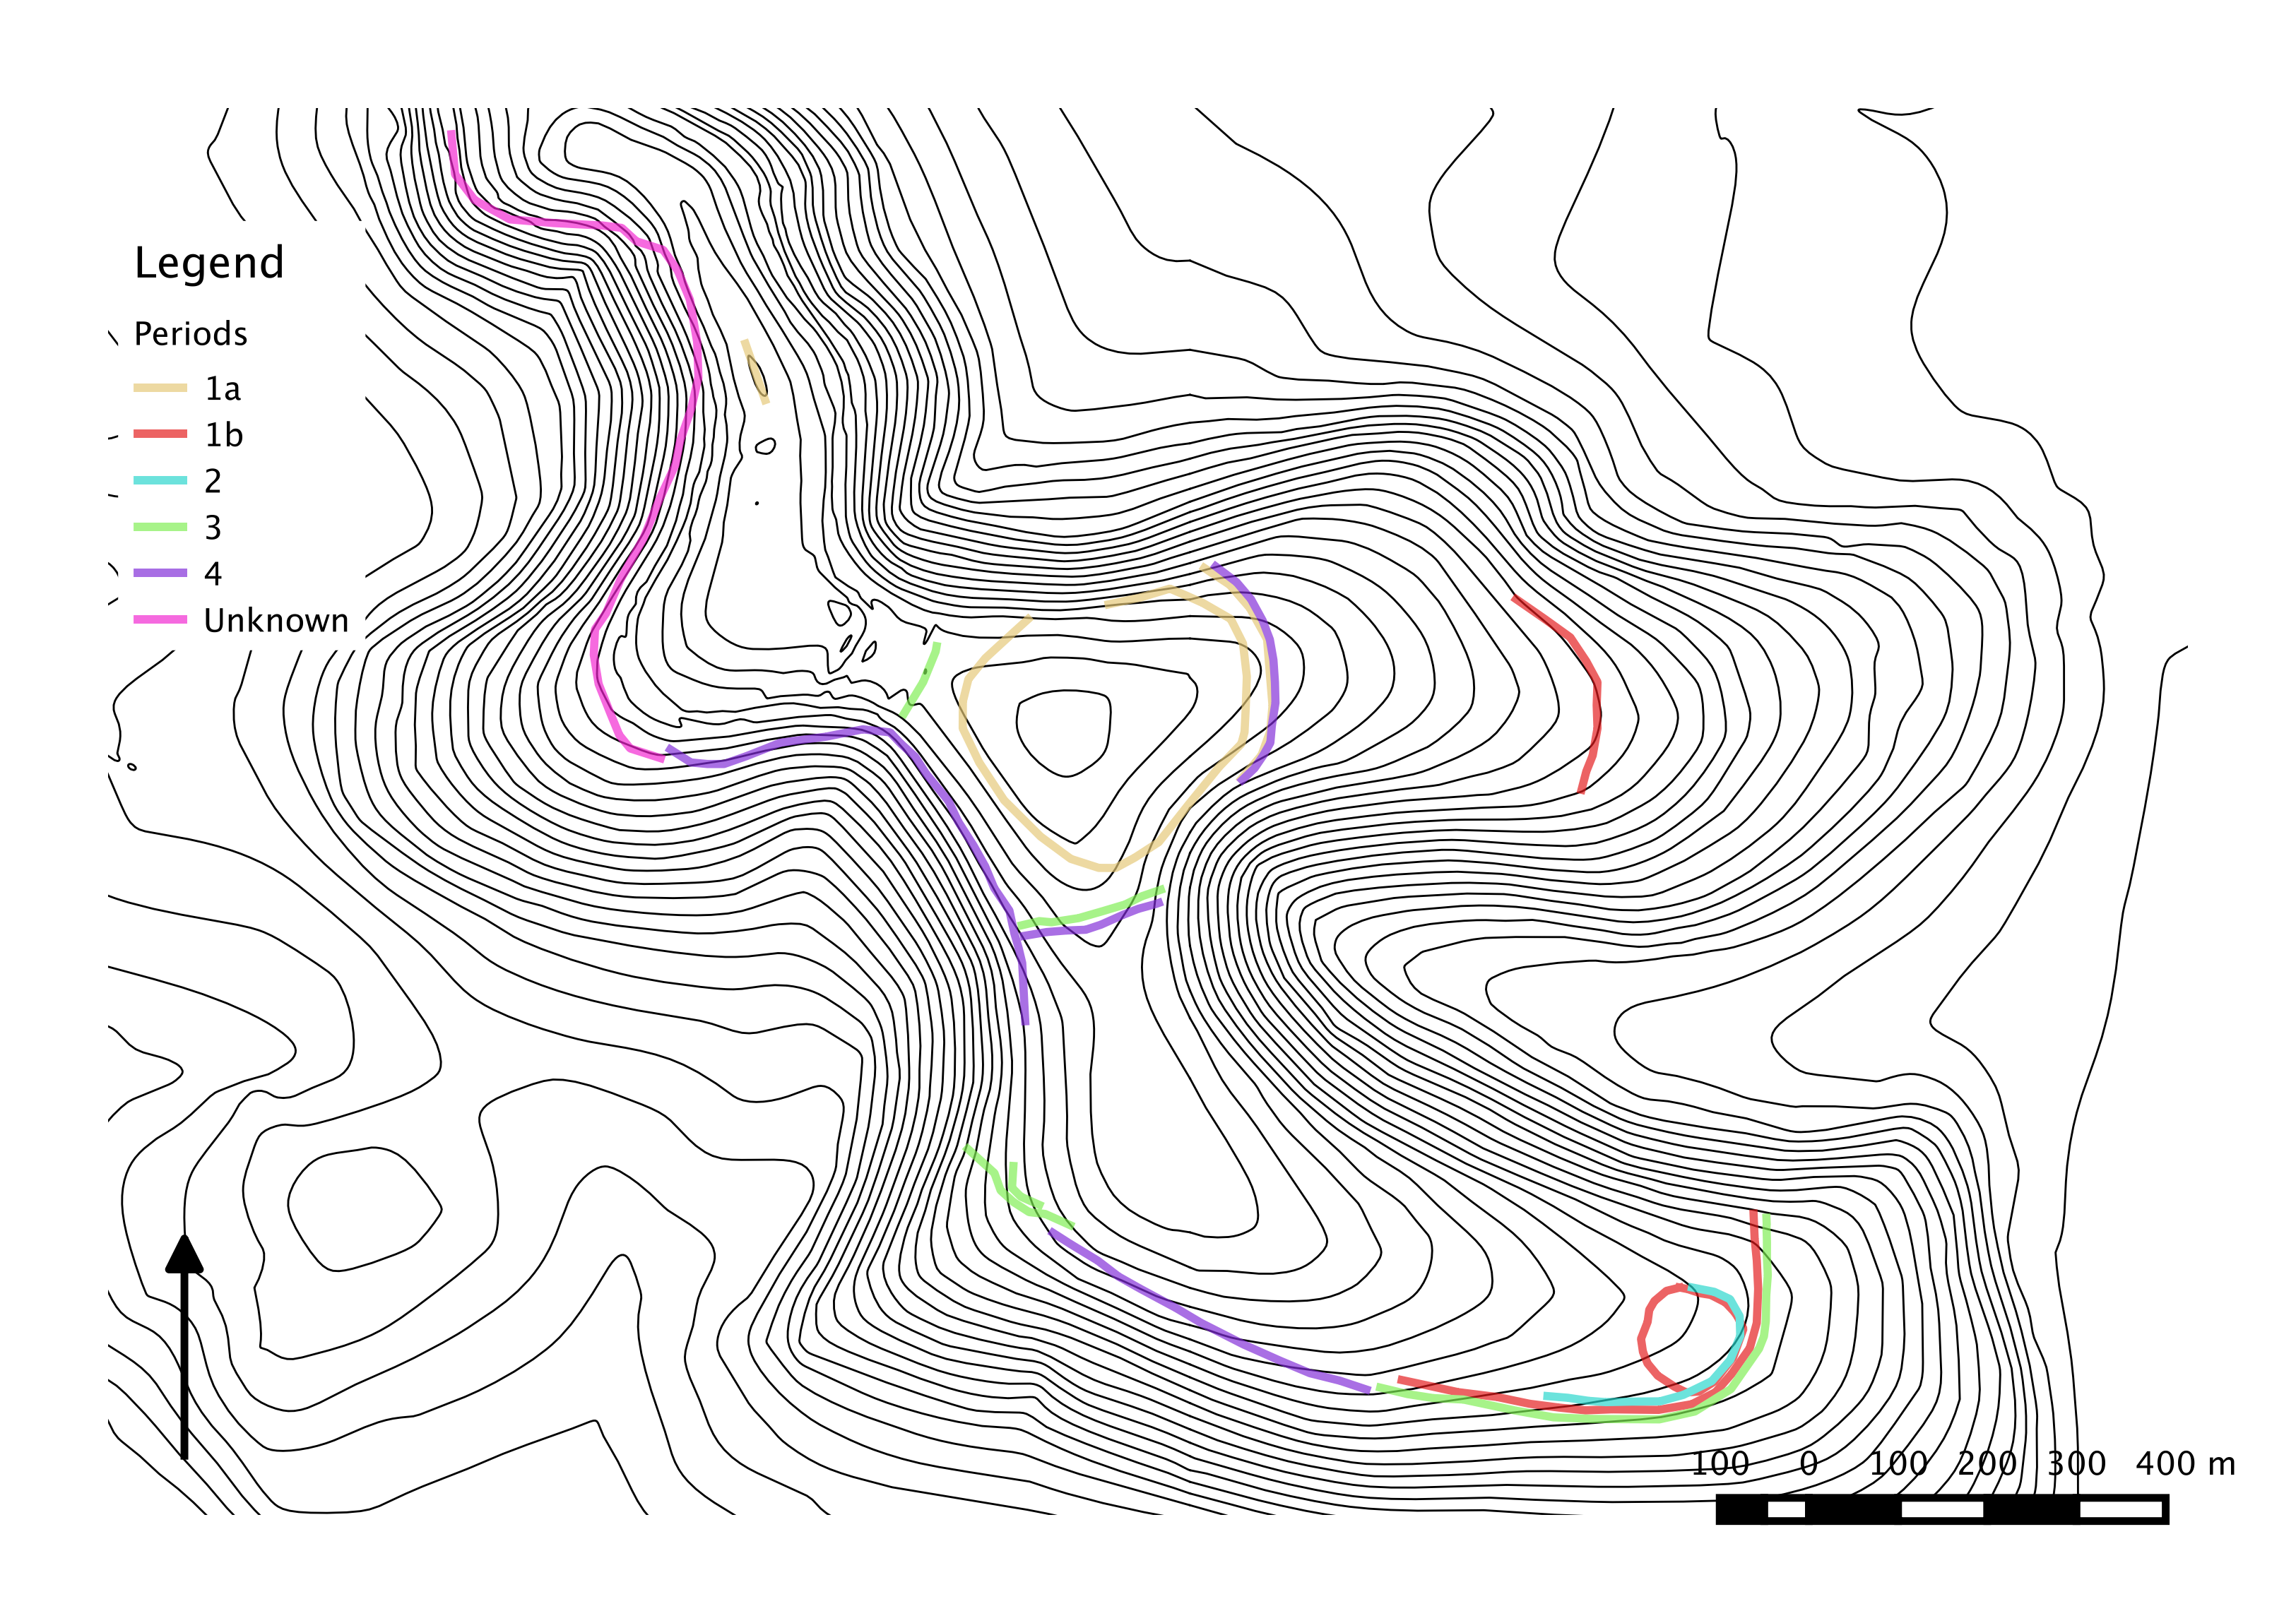
\includegraphics[width=0.9\textwidth]{figures/periods}
\end{center}
  \caption{Development of the Hambledon Complex by period, after \cite{Mercer:2008fk}}
  \label{fig:periods}
\end{figure}

The primary temporal evidence for Hambledon Hill comes from the the bayesian analysis documented in \citet{Whittle:2011kl}. This builds upon the original bayesian analysis, which formed a part of the report by \citet{Mercer:2008fk}. These analysis resulted in the definition of a sequence of discrete chronological periods of the site's Neolithic development, see figure~\ref{fig:periods}. The bayesian analysis was conducted using a subset of the radiocarbon dates combined with a model of the sites chronology, based on excavation evidence. 

\subsection{Pre-Neolithic Evidence}
The unequivocal temporal evidence for use of the site prior to the Neolithic comes from two areas, WOWK3 F4 and HN82 F279, plotted on figure~\ref{fig:meso1}. The feature WOWK F4 is interpreted as a likely Boreal age post in the original publication \citep[46]{Mercer:2008fk} on the basis of the compactness of the sample, and the lack of other charcoal samples of contemporary age from the surrounding area. This reduces the likelihood that it came from an episode of wider Boreal vegetation burning and subsequent redeposition. It is dated by one radiocarbon measurement (OxA-7816) to 8160-7590 cal B.C. \citep[43]{Mercer:2008fk}. 

\begin{figure}
\begin{center}
	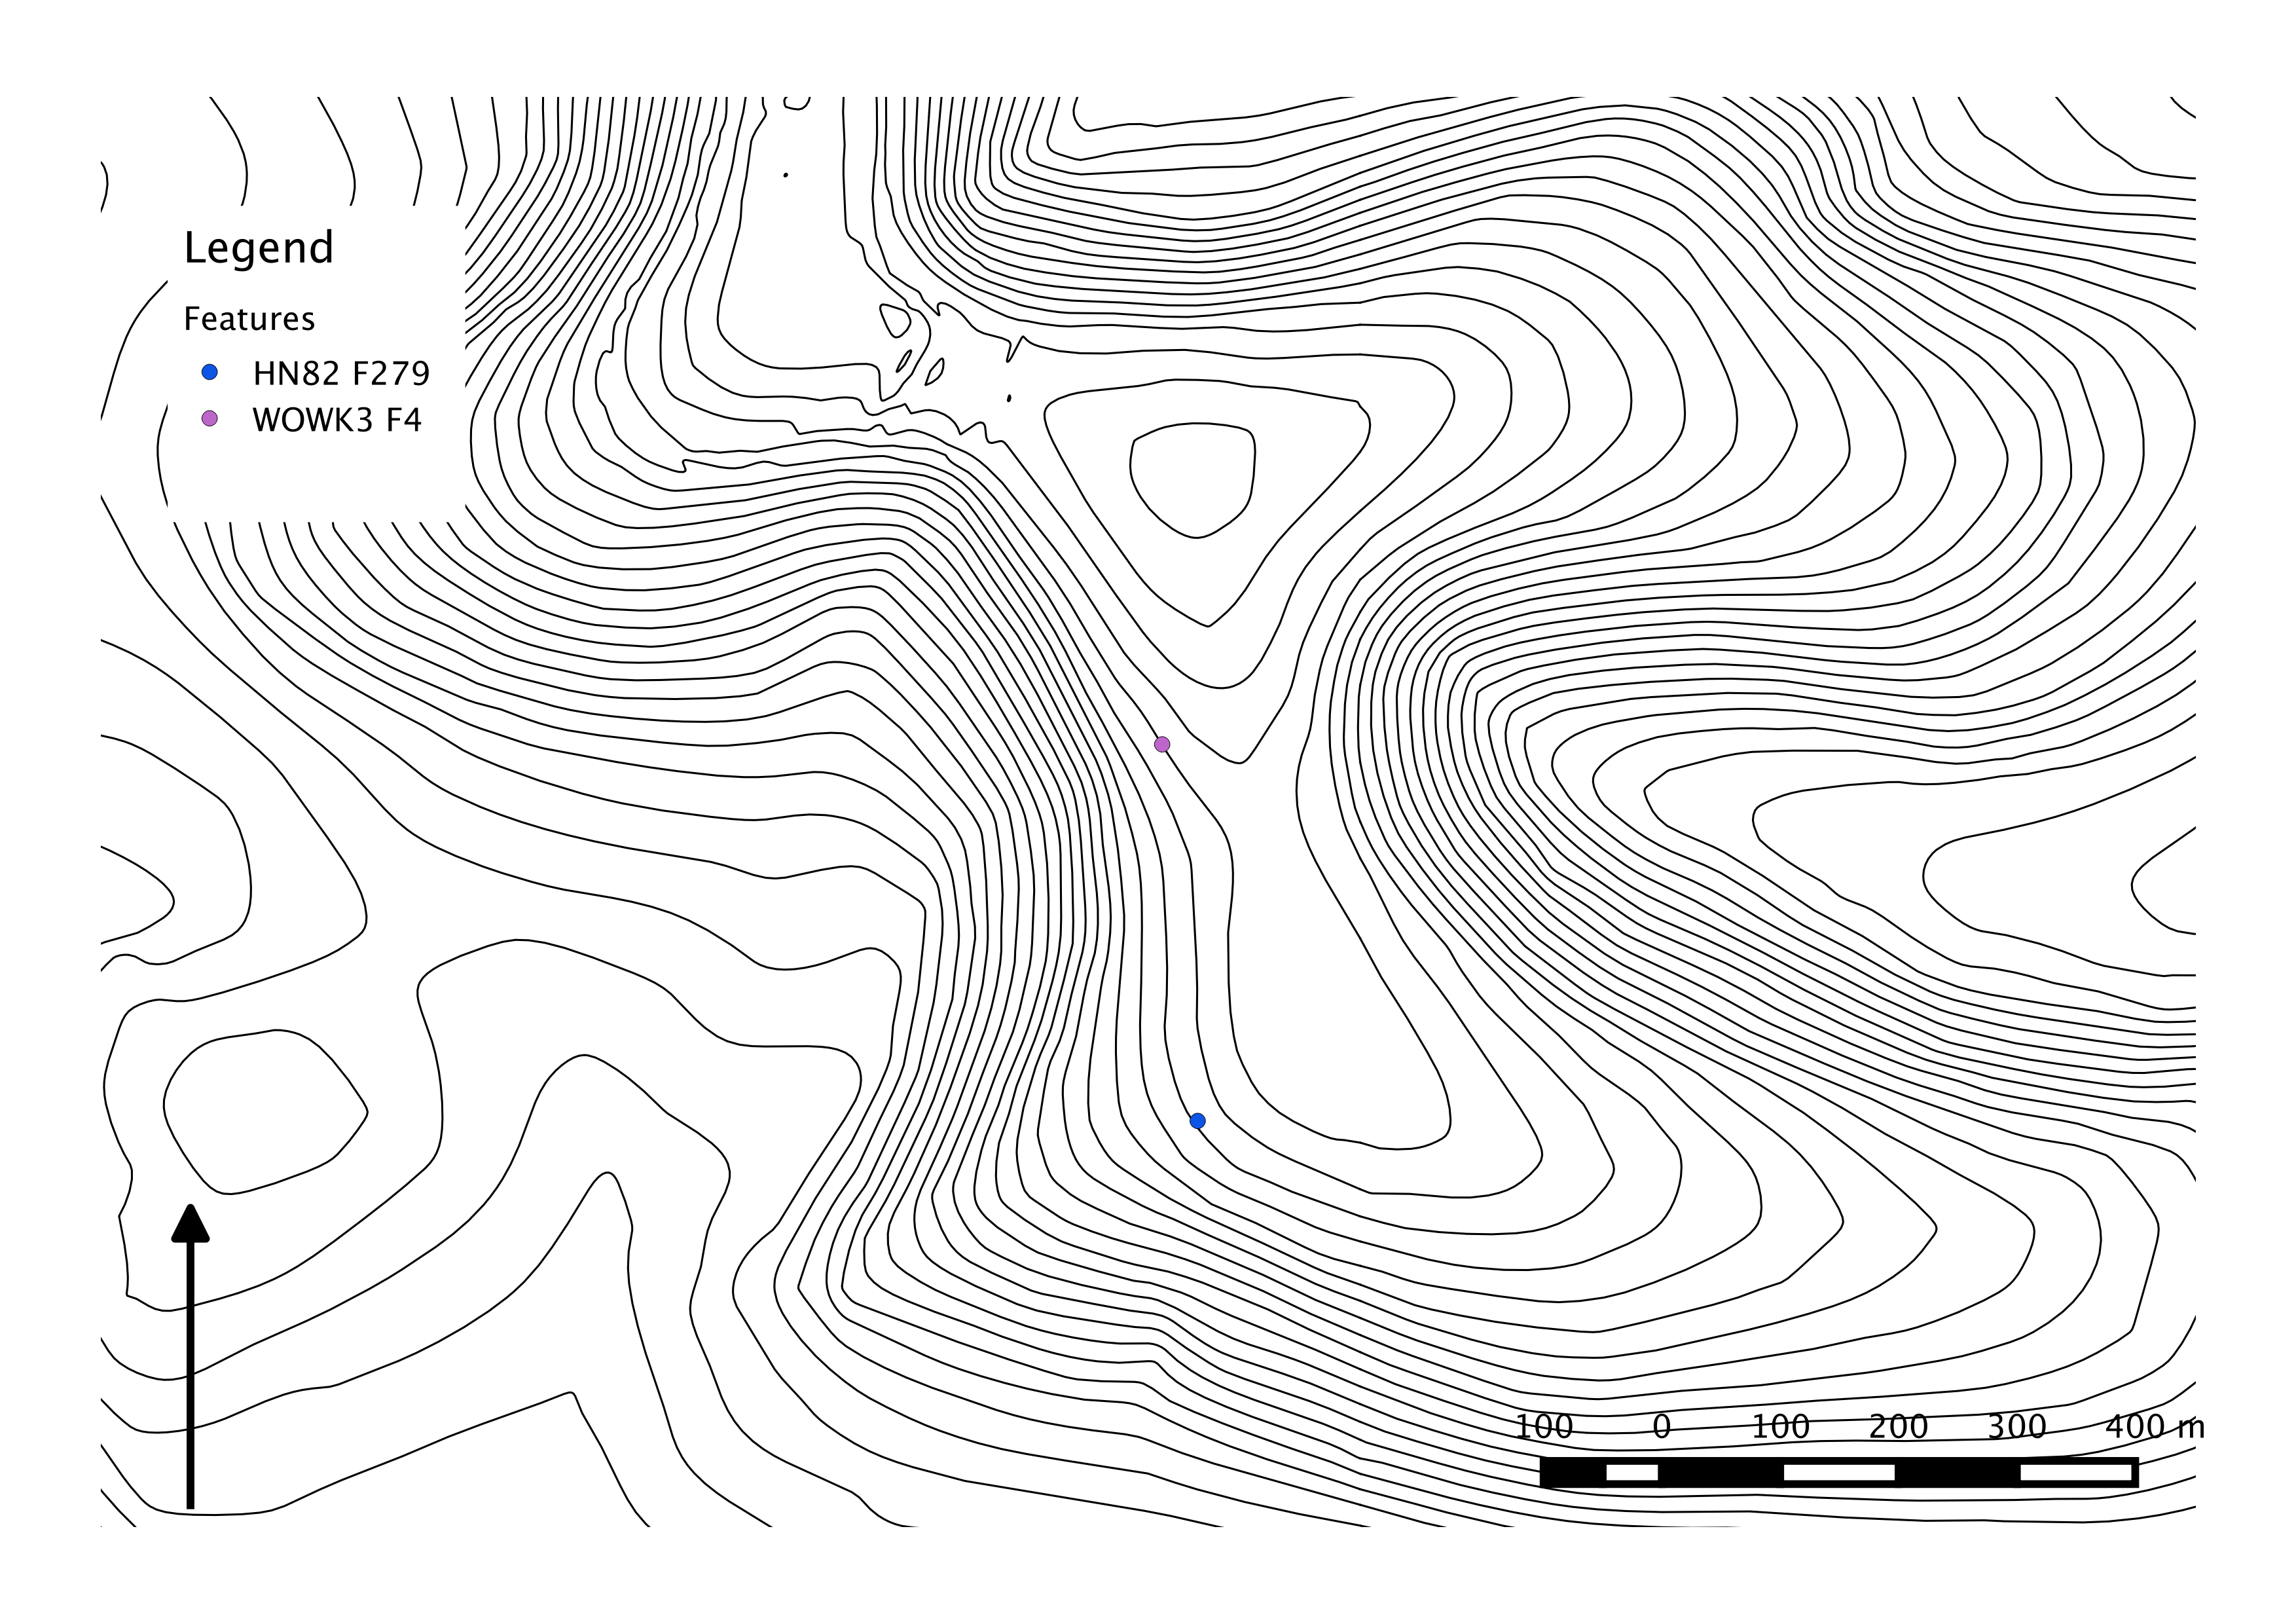
\includegraphics[width=0.9\textwidth]{figures/meso-features}
\end{center}
  \caption{Location of features containing Mesolithic dated samples}
  \label{fig:meso1}
\end{figure}

Feature HN82 F279 is much larger than the other, and is compared in the original report to the large pine posts, of a similar date, which stood near Stonehenge \citep[48]{Mercer:2008fk}. It was dated by two radiocarbon measurements (OxA-7845 and OxA-7846) giving dates of 7580-7200 cal B.C. and 7600-7380 cal B.C. \citep[46]{Mercer:2008fk}. The report also mentions feature F773 (undated) as being similar in form to F279 and the authors suggest the two are comparable \citep[46]{Mercer:2008fk}. There is also a third feature, F507, although the authors are less convinced by its comparability, suggesting it may instead be a part of the Neolithic bank structure. They are both from the same trench as F279.

Finally on the Stepleton spur, feature 4C F500 is identified by the authors as of a similar form to the features mentioned above, \citep[48]{Mercer:2008fk} but it has not been dated. 

Clearly there is evidence for activity on Hambledon Hill preceding its Neolithic use, although this evidence is relatively thin by comparison to later periods. The limited evidence available is focused on the West and South-West of the Hill, however feature 42 F500, if it were of a similar date, would show activity also took place on the opposite side.

\subsection{Pre-Neolithic and Neolithic Activity in the wider landscape}
There is also evidence of activity in the vicinity of Hambledon pre-dating and coinciding with its Neolithic use, the dating evidence is covered in \citep[151]{Whittle:2011kl}. This evidence comes from the Dorset Cursus, the Firtree Field Shaft, Thickthorn Down Barrow, Wor Barrow and the Monkton-up-Wimborne complex. The first three of these sites, along with the Hambledon features are shown on figure~\ref{fig:meso2}.

\begin{figure}
\centering
	\includegraphics[width=0.9\textwidth]{figures/meso-area}
  \caption{Location of pre-Hambledon Neolithic sites in the locality}
  \label{fig:meso2}
\end{figure}

This activity is mostly much more recent than the Boreal activity on Hambledon itself and overlaps the start of the main Neolithic use of the site. The evidence is clearly limited, for example the dating of Thickthorn Down is based on one radiocarbon sample, which may have been contaminated \citep[155]{Whittle:2011kl}. There is more evidence from the Dorset Cursus and Fir Tree Field shaft, however both of these were clearly in use for a long period of time. Any regularity, or evidence for continuous use is unclear from the models and radiocarbon dates. The case of the Cursus may not be helped by the potential for activities that attempted to keep it clean or clear. 

Crucially the Fir Tree Field shaft contains the earliest evidence for Neolithic activity in the area, a hearth associated with Neolithic Bowl pottery, dated to 3960-3755 cal BC (89\% probability, OxA-8009) or 3745-3710 cal BC (6\%) and probably to 3945-3850 cal BC (46\%) or 3845-3830 cal BC (5\%) or 3825-3785 cal BC (17\%) \citep[155]{Whittle:2011kl}.

\subsection{The Neolithic Complex}

\begin{figure}
\centering
	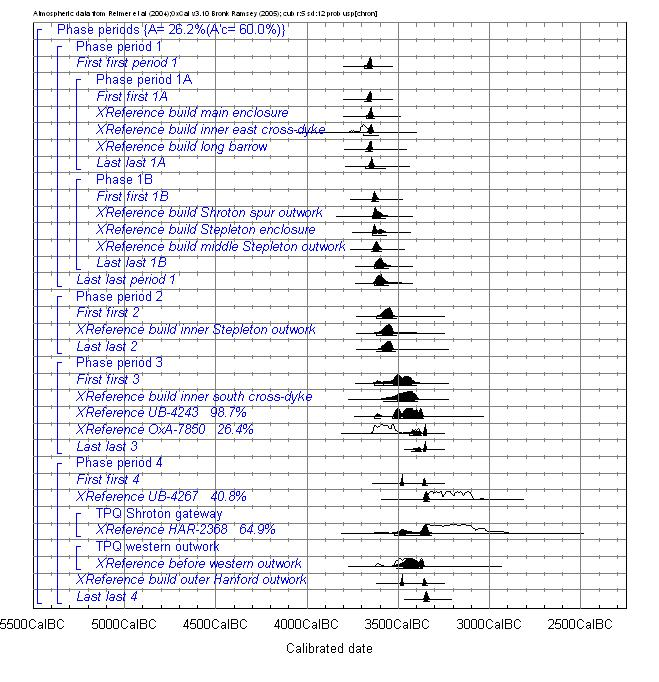
\includegraphics[width=0.9\textwidth]{figures/period-model}
  \caption{Posterior density estimates for the construction of the Neolithic earthworks and for the periodisation of the complex. Figure 4.14 from \citep[151]{Whittle:2011kl}}
  \label{fig:period-model}
\end{figure}

The results from the bayesian modelling were used to create a series of phases, reproduced as  figure~\ref{fig:period-model}, these are the same periods shown in figure~\ref{fig:periods}. This plan shows how the series of earthworks was built up across five discrete periods, although it does not show later re-use or re-cutting of earlier features. The original model is split based on geographic location in the original volumes, so that is how it shall be considered here.  

These bayesian models include a subset of the radiocarbon dates for the site, used to build a formal chronological model. However they lack any spatial reference. Using these models, plus the context information for each sample, it is possible to plot the rough location for each dated sample, shown in figure~\ref{fig:dates}. What this shows is concentrations of dates in certain parts of this site, clearly these are the excavated areas, however large sections of earthwork, which have been presented as part of the dated periods, have no associated dating evidence whatsoever. 

\begin{figure}
\centering
	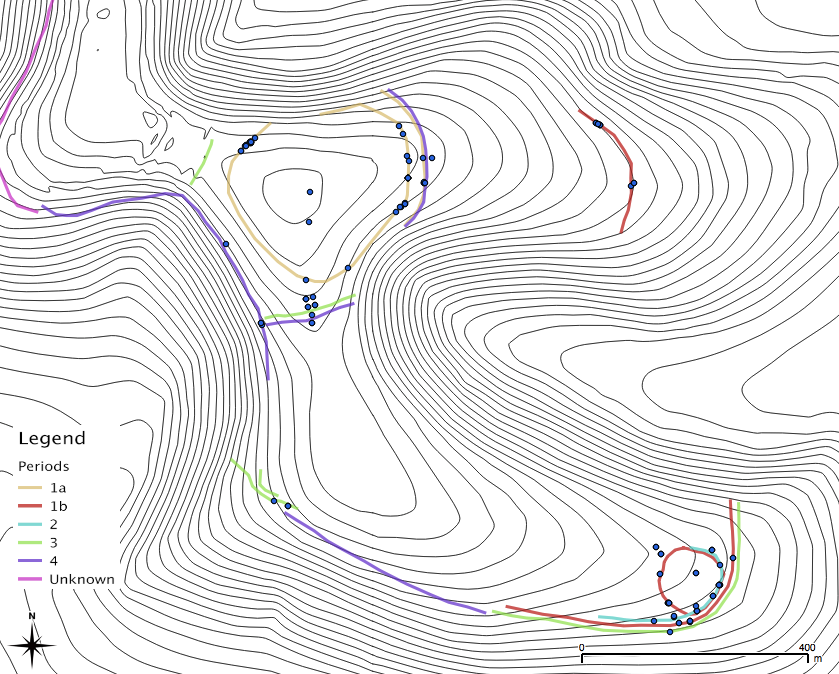
\includegraphics[width=0.9\textwidth]{figures/dates}
  \caption{Plot of the locations of all samples included in the bayesian model for the site, and key earthworks, for reference.}
  \label{fig:dates}
\end{figure}

\begin{figure}
\centering
	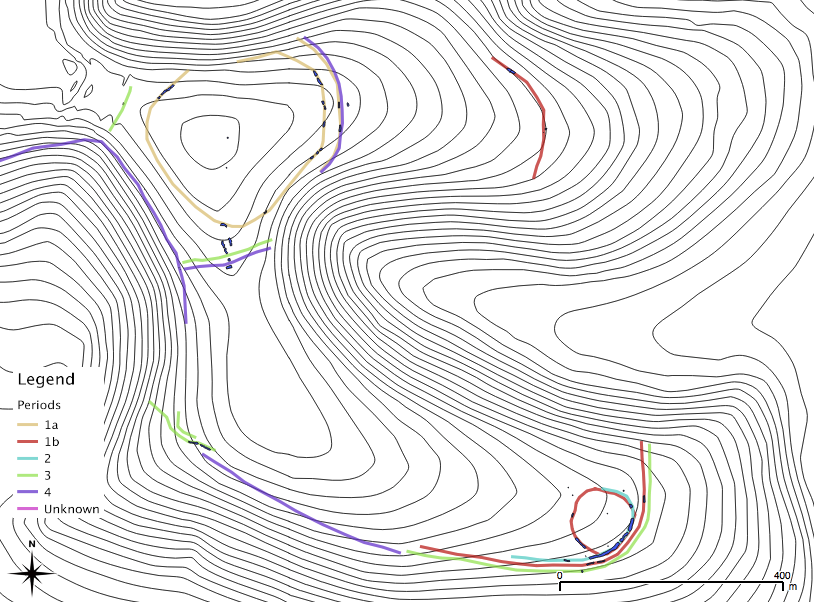
\includegraphics[width=0.9\textwidth]{figures/dated-features}
  \caption{Plot of all features dated via the bayesian model, and key earthworks, for reference.}
  \label{fig:dated-features}
\end{figure}

This in itself is not the spatial basis for discussion, instead the contextual information for each radiocarbon sample also specifies which ditch segment (or pit) it came from. These have been chosen as estimate find spots as the date locations are often only down to the segment and a point on a map therefore carries a misleading accuracy. Also assuming the date is a valid proxy for activity in the segment, such as its construction, or some form of use, and is not residual or incursive, then we can attribute that date to the feature, or an event involving it. Even more useful is when there are several dated samples, which have been included in the model, in this case we might have dates for multiple events involving the segment, and therefore a clearer idea of when that feature was in use. Rather than considering such dates independently, it makes sense to combine them spatially, as they all relate to the same segment, and are therefore not independent observations. Figure~\ref{fig:dated-features} shows for the whole site those features which have been dated via the bayesian model, overlain on the earthworks, by period. 

\subsubsection{The Central Area}
The central area of Hambledon Hill covers the causewayed enclosure, built during phase 1a. The dating evidence for this is modelled in two diagrams in \cite{Whittle:2011kl}. Figure~\ref{fig:central1} and figure~\ref{fig:central2} shows these two diagrams along with plans of the features dated by each model.

\begin{figure}
\centering
	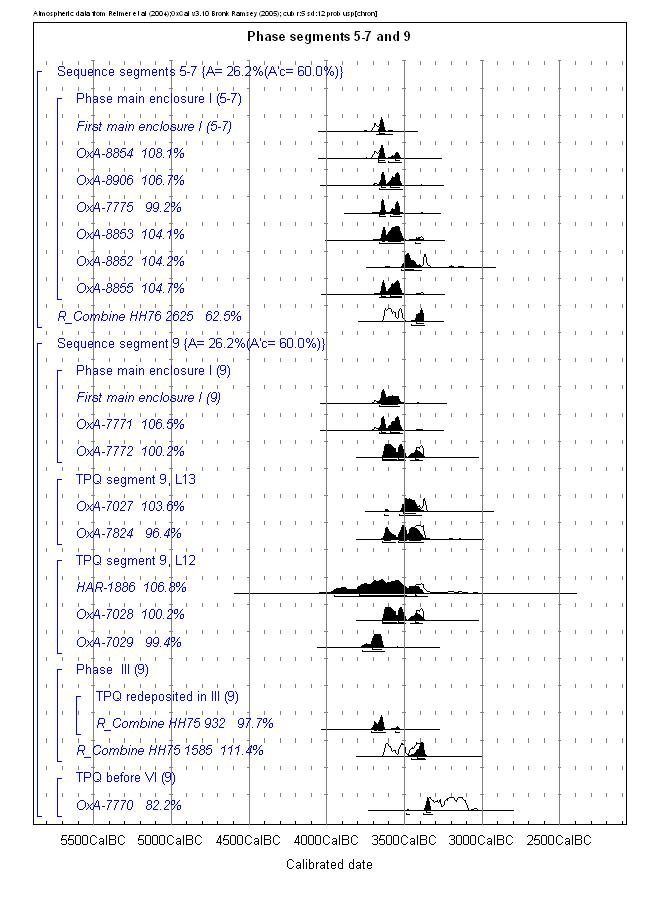
\includegraphics[width=0.7\textwidth]{figures/model1}
	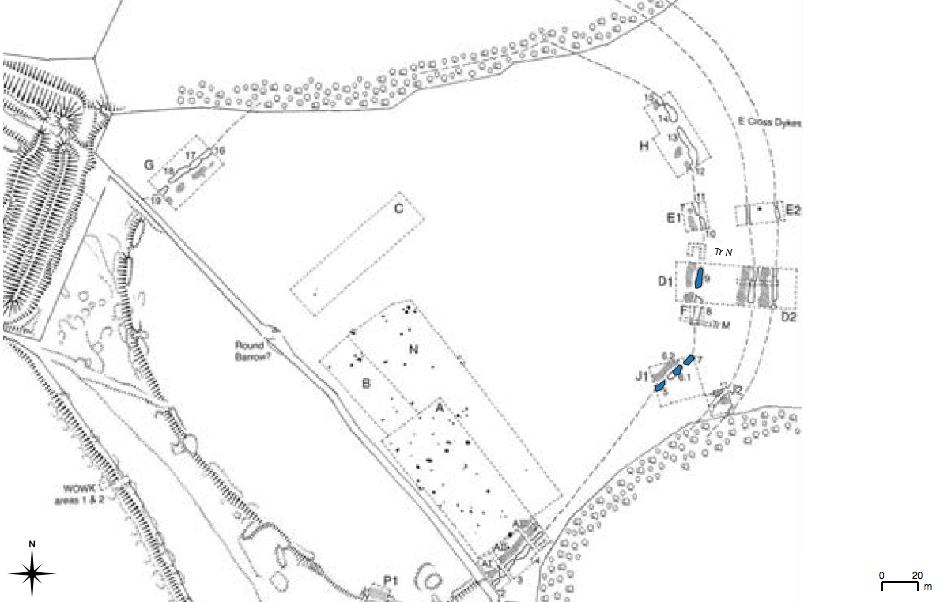
\includegraphics[width=0.9\textwidth]{figures/model1-plan}
  \caption{Bayesian model for the central area and plan of the features dated, from fig 4.8 \citep[139]{Whittle:2011kl}}
  \label{fig:central1}
\end{figure}

What becomes immediately clear, is that within the excavated areas, there is good coverage of the bayesian model on ditch segments for the central causewayed enclosure. Figure~\ref{fig:central1} is more localised in the South-East, where as figure~\ref{fig:central2} covers the remaining excavated areas. Having said that, figure~\ref{fig:central1} only covers four ditch segments, and figure~\ref{fig:central2} covers ten, combined they perhaps date around one third of the ditch for the causewayed enclosure on Hambledon Hill. 

\begin{figure}
\centering
	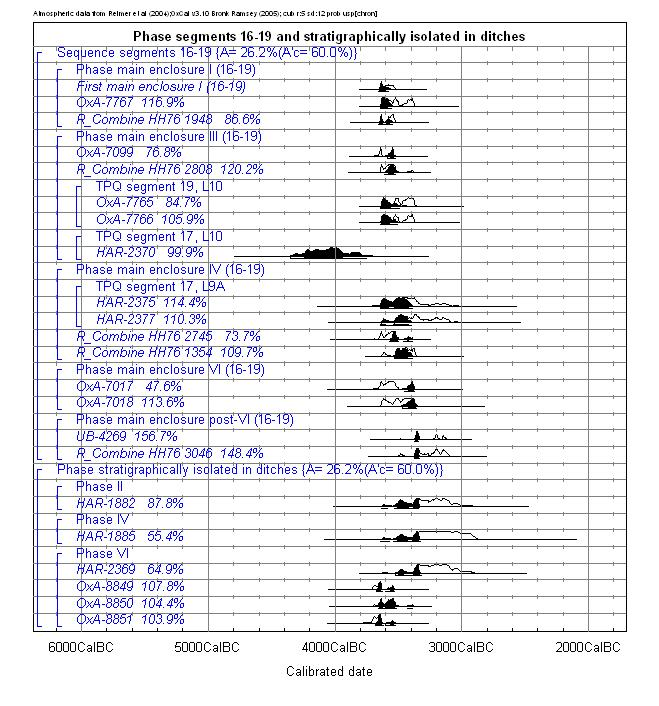
\includegraphics[width=0.7\textwidth]{figures/model2}
	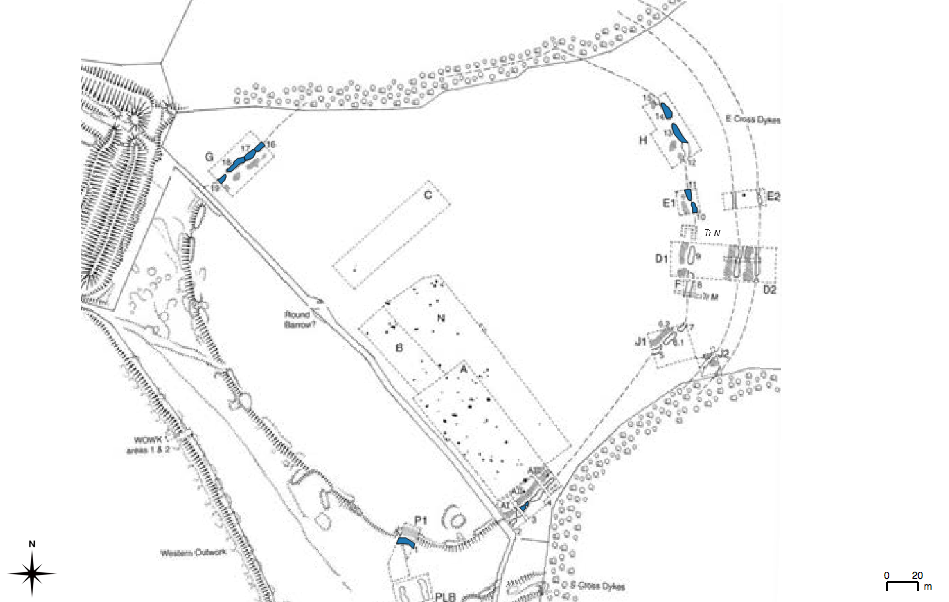
\includegraphics[width=0.9\textwidth]{figures/model2-plan}
  \caption{Bayesian model for the central area and plan of the features dated, from fig 4.9 \citep[140]{Whittle:2011kl}}
  \label{fig:central2}
\end{figure}

However several of the ditch segments dated in figure~\ref{fig:central2} are included under the model as ``stratigraphically isolated in ditches''. These are included primarily as additional dates for phases where dated evidence is scarce, providing a comparison to make sure other dates are not residual or incursive. The approximate locations of those dates included in the stratigraphically isolated section is shown in figure~\ref{fig:central-isolated}. When these are excluded the dating evidence from the primary fills of the causewayed enclosures comes from two sections of ditch segments, segments five to seven, nine and 16-19. All of the dates from these two sections of ditch segment are included in table~\ref{tab:central-dates} along with details about which segment they came from, and phase.

\begin{figure}
\begin{center}
	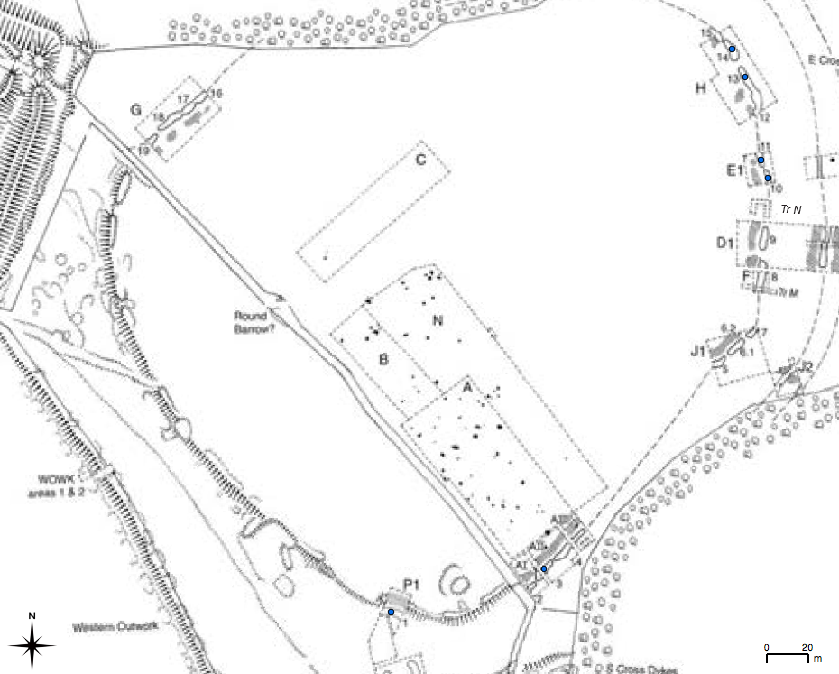
\includegraphics[width=0.9\textwidth]{figures/central-isolated.png}
\end{center}
  \caption{Plot of all locations of dates identified as stratigraphically isolated in fig 4.9 \citep[140]{Whittle:2011kl}}
  \label{fig:central-isolated}
\end{figure}

\csvautolongtable[
  table head= \caption{List of all dates included in the bayesian model of the central area, the calibrated date is at the 95\% confidence interval}\label{tab:central-dates} \\\hline
               \csvlinetotablerow\\\hline
               \endfirsthead\hline
               \csvlinetotablerow\\\hline
               \endhead\hline
               \endfoot,
]{figures/central-dates.csv}

There are six dates for the first phase (phase I in the original report) from segments five to seven, grouped as ``Phase main enclosure I'' \citep[139]{Whittle:2011kl} of these OxA-8852 stands out as it is not statistically significant with the rest, and is in fact significantly younger \citep[398]{Mercer:2008fk}. OxA-8852 is one of two dates from segment 6.2, the other is assumed to be redeposited on the basis that it is younger, despite being consistent with the dates from other segments. For these segments the only other dated event is the end of Phase II, which is dated by a sample from segment 6.2. The next segment, segment nine, while included with five to seven in the original model, and discussion, is in fact from a distinct area of the excavation. In this segment phase I is dated by two samples, phase II is dated by charcoal samples, which are treated as a terminus post quem. Phase III contains samples consistent with the underlying layers and but also potentially redeposited samples. Segments 16-19, are on the opposite side of the circuit to five to seven, here phase I and II are dated by samples from a child burial cut into the base of segment 18, and also bone fragments from segment 16. Phase III is dated by a terminus post quem from segment 17, and one also from segment 19. Phase IV and phase VI are dated by samples from segment 17. Across these areas, there are 11 dates from phase I, five from phase II, two from phase II / phase III interface, ten from phase III, six from phase IV, three from phase VI and three post phase VI. Clearly phases I to III make up the bulk, at 18 samples, where as phases IV and beyond are only dated by 12 samples. When considered from a purely temporal perspective this looks to be a good set of dates, however this is only looking at the data from a one dimensional perspective. When the spatial dimension is included, it becomes clear that the distribution is far from even. The phase I and II samples are mostly from the areas of segment five to seven and nine, and phase III samples are split between segments nine, 17 and 19. And phase IV, IV and post-IV are almost exclusively from segment 17.

The original report found that the enclosure was likely built in a short span of time, although not necessarily at the same time, based on the consistent results provided by the 11 samples (if OxA-8852 is excluded) and the nature of the samples, coming mostly from articulated or articulating deposits \citep[401]{Mercer:2008fk}. But when we look at those areas on a plan, we can see that the earliest evidence for the causewayed enclosure comes from a small group of segments on one side of the circuit, and one segment on the opposite side. The original report used this as evidence that the whole circuit was built in a relatively short period of time. This is one interpretation, it could also be that the two areas dated were constructed at the same time, but not necessarily the entire circuit. If we include the spatial evidence that these two areas were almost exactly opposite this could be interpreted as evidence that opposite sides of the circuit were worked on at a similar time. While the evidence does support the original conclusions about the construction of the enclosure, it is open to alternative interpretations, the limited nature of the evidence, in particular its spatial spread is a constraint on our knowledge about the construction of the ditch circuit. By considering the spatial pattern the original conclusions are less secure than they initially appeared. 

\subsubsection{Cross Dykes and the Long Barrow}
This model shown in figure~\ref{fig:crossdykes} is a bit of a ``catch all'' for those parts of the site that do not fit into the other main areas, instead forming a periphery to the central area.

\begin{figure}
\centering
	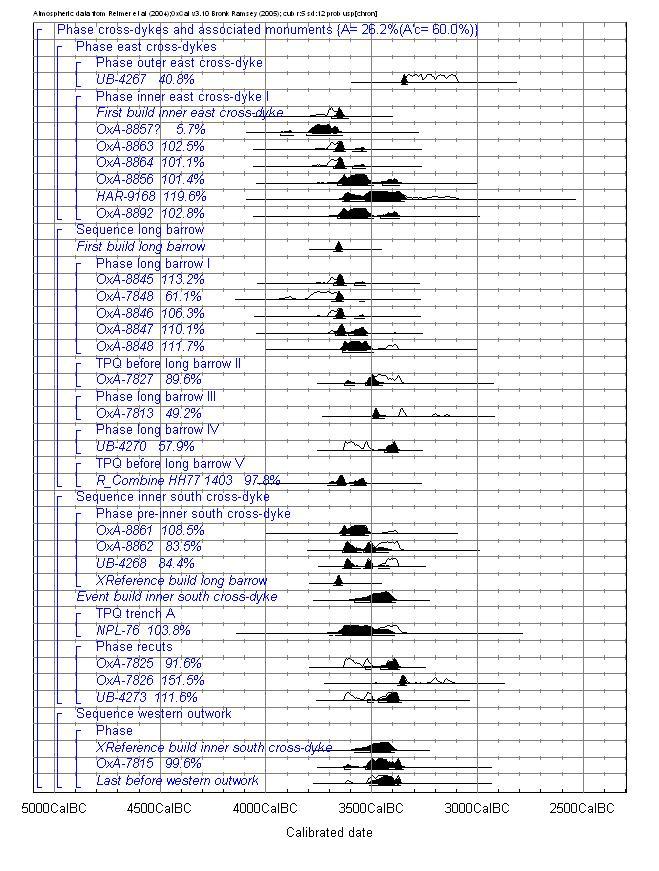
\includegraphics[width=0.7\textwidth]{figures/model3}
	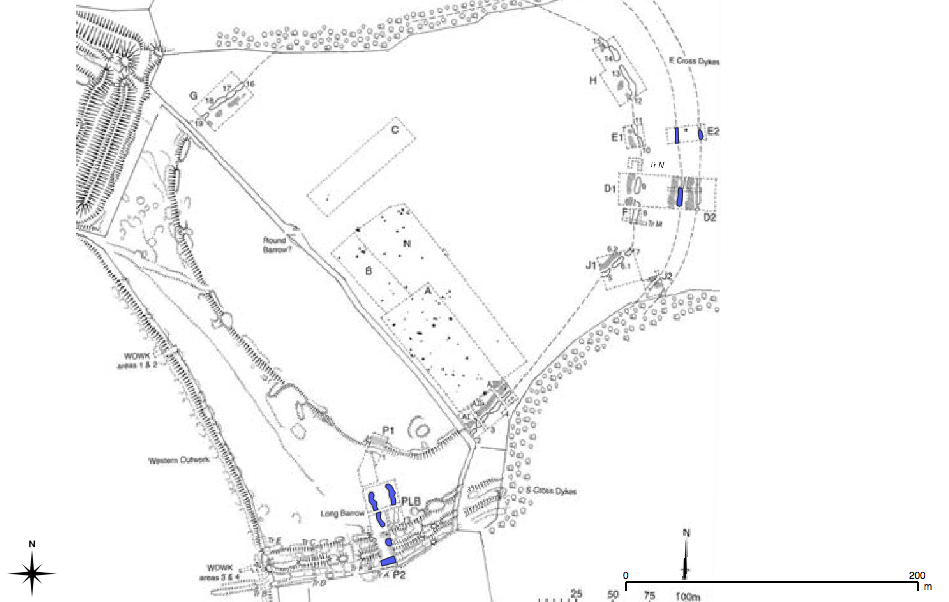
\includegraphics[width=0.9\textwidth]{figures/model3-plan}
  \caption{Bayesian model for the cross dykes, etc and plan of the features dated, from fig 4.10 \citep[139]{Whittle:2011kl}}
  \label{fig:crossdykes}
\end{figure}

Firstly, the east cross-dykes, the outer east cross-dyke only gave one date, UB-4267, which calibrated to 3360-2700 cal B.C. (95\% confidence) \citep[122]{Whittle:2011kl}. This is considerable later than the dates for the inner east cross-dyke and for most of the rest of the central area. It is possible that the dated material is in fact from an extension of the original segment \citep[401]{Mercer:2008fk} and as the date is closer to those of recuts of the south cross-dyke it could represent a phase of broader re-furbishment of the site. However, with only one date to go on, this is purely speculative, and when examined on a plan of the site, the two areas are quite far apart, making some coincidental localised recutting and extending an equally likely proposition. 
 
The inner east cross-dyke, having five dates included in the model provides a bit more to go on, however four were from the same segment, segment four. Of these, three were taken from charcoal and one was a bulk sample (HAR-9168). OxA-8856 came from a red deer antler tip, and OxA-8892, in segment five, a cattle radius fragment. \citet[401]{Mercer:2008fk} note that all of these measurements are statistically significantly different. \citet[136]{Whittle:2011kl} state that the cross-dykes were built at the same time as the main enclosure. Based on the limited evidence available this does not seem particularly contentious, but the evidence for the east cross-dykes is very limited spatially, and also temporally, as all the samples are from phase I.
 
The south long barrow was extensively excavated, as shown in figure~\ref{fig:crossdykes} and the dates for it come from three quadrants. In total it produced ten dates that were included in the model, of which half came from phase I, two came from a TPQ before phase V and the rest were one per phase for II, III and IV \cite[401]{Mercer:2008fk}. These last three all came from quadrant LB3, where as the five for phase I came mostly from LB2, with one coming from LB4. While it seems highly likely that a monument such as this would have been constructed in one go, it would have been preferable to have a continuous chronology from a single area. Especially as all these dates came from the ditches, so it is possible that the dates for later phases may be activity in a specific quadrant or side of the long barrow.

Next on the model is the inner south cross-dyke, sealed beneath the cross-dyke were several samples pre-dating the bank construction, one UB-4268, a cattle tibia fragment. OxA-8861 and OxA-8862 are from a possible post hole, treated as a terminus post quem \citep[402]{Mercer:2008fk}. These samples are not included in figure~\ref{fig:crossdykes} as it was not possible to determine their spatial location from the information included in \cite{Whittle:2011kl} and the plans in \cite{Mercer:2008fk} are not reproduced at a high enough quality to identify the feature in WOWK area three. The features dated by other samples in the model are only rough approximations, as the plan in \cite{Mercer:2008fk} is a low quality reproduction, and is quite confused in this area of the site. Only one of the samples is from phase I, but it is a bulk sample containing oak charcoal and so has a broad posterior, it is only usable as a terminus post quem. The other samples are later, from phase VI. Clearly, a spatio-temporal assessment of the inner south cross-dyke is problematic as it is very difficult to determine the positions of the features dated. What we can determine is that the possible post hole, which may pre-date the bank, or be part of its structure \citep[402]{Mercer:2008fk} is at the western-most end of the cross-dyke, whereas the datable material is from its center.

Finally in this model is the western outwork. This is also not included in the plan in figure~\ref{fig:crossdykes} as, while the location of WOWK area two is marked, the features excavated are not. Without a clearer plan, or more information it would only be possible to locate this date to the excavated area. In summary, these features on the periphery of the central area are, apart perhaps from the long barrow, generally lacking in dating evidence, especially in terms of  spatial spread. 

\subsubsection{Stepleton Enclosure and Outworks}

\begin{figure}
\centering
	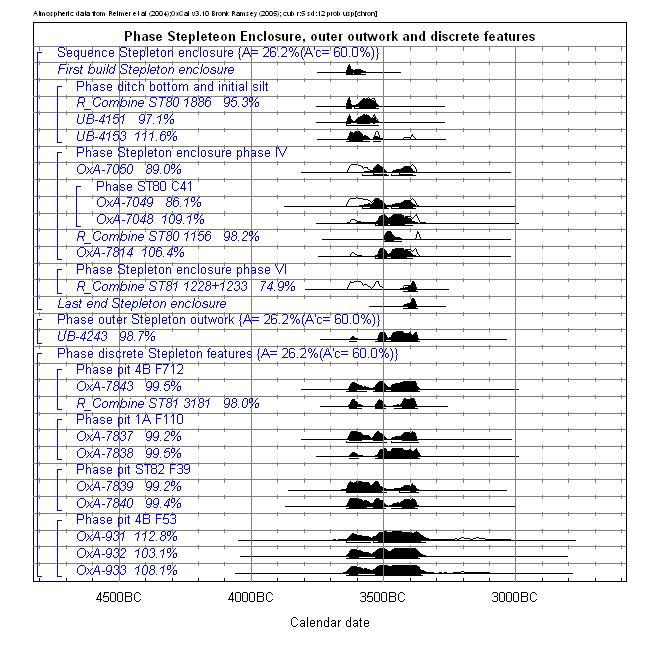
\includegraphics[width=0.7\textwidth]{figures/model4}
	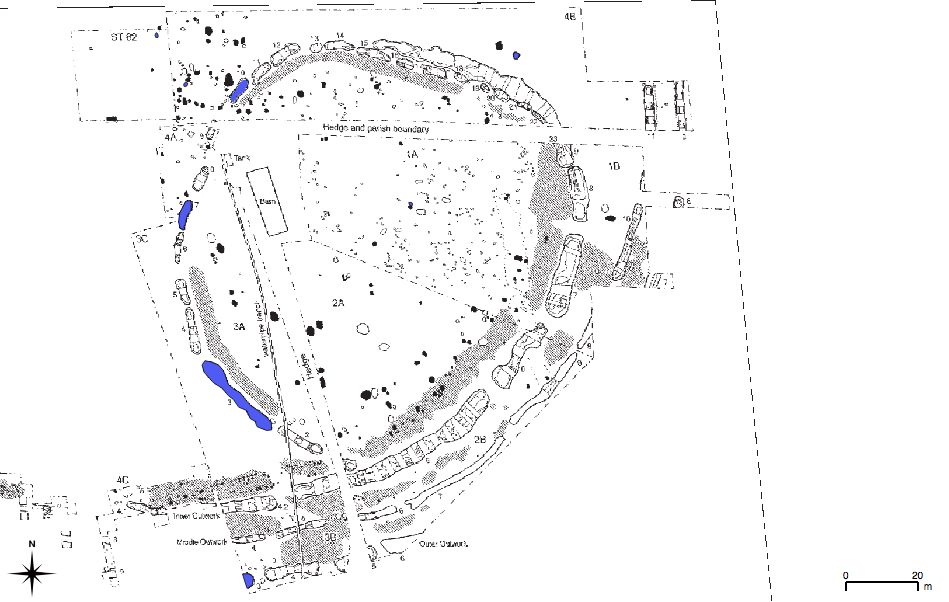
\includegraphics[width=0.9\textwidth]{figures/model4-plan}
  \caption{Bayesian model for the Stepleton enclosure and plan of the features dated, from fig 4.11 \citep[142]{Whittle:2011kl}}
  \label{fig:stepleton}
\end{figure}

The Stepleton enclosure is a causewayed enclosure with a series of outworks, to the south-east of the main enclosure. Figure~\ref{fig:stepleton} shows the bayesian model for this area, from fig 4.11 \citep[142]{Whittle:2011kl} and a plan of the excavation, with the ditch segments and pits that have contributed dates to the model highlighted in blue. The plan shows that the dates for the enclosure come from three ditch segments and four pits, of which one is inside the enclosure and the other three are outside. This model also provides a date for the outer outwork, with one segment being dated. 

The initial construction of the ditch is dated by five measurements on three antler implements, from the base of ditch segment three, these are assumed in the original report to be close in age to the ditch's excavation \citep[394]{Mercer:2008fk}. There are no dates included in the bayesian model for phase II or phase III which makes up most of the fill, phase IV is dated by short life charcoal from a pit cut into the fills, (OxA-7048, OxA-7049, OxA-7050) and samples from an articulated dog skeleton (UB-4138 and OxA-7041). Also included in the model for phase IV is a sample from segment ten, from an articulated upper body of a woman (OxA-7814). To complete the sequence, two dates were taken from segment seven, from samples of sooty residue on two sherds, however the original report notes that these two samples were statistically significantly different \citep[394]{Mercer:2008fk}. Clearly the main focus of this part of the model is on segment three, although we can see from the plan in figure~\ref{fig:stepleton} that this was a large segment and it is not clear whether all the dates were taken from samples found close together, or at opposite ends of the segment. The additional dates from segments seven and ten rely on the phases being comparable across the different segments, and dating the whole enclosure from this limited evidence relies on the phases being comparable across the whole enclosure. \citet[394]{Mercer:2008fk} note ``it is impossible to tell if the sequence in every segment is synchronous'' which is unfortunate, as this is clearly a requirement for combining dates from multiple segments into the same phases and for extrapolating the dates of these phases across the wider area.

Five discrete features within and around the Stepleton enclsoure were also dated, only four shall be considered here, as feature 1A F70 an articulated child burial (dated by OxA-7836) was accidentally missed out when the model was rebuilt for Gathering Time (Alex Bayliss, personal communication) and so does not feature in the model shown in figure~\ref{fig:stepleton}. The other internal feature 1A F110 contained a deposit of barley, dated by OxA-7837 and OxA-7838. 4B F712 was also a burial, to the north-east exterior of the enclosure, with two samples from the skeleton dated (OxA-7818 and UB-4311) and one from charred hazelnut shells (OxA-7843) \citep[396]{Mercer:2008fk}. The other two features were both to the north-west exteriors, one, ST82 F39 dated by a quantity of emmer wheat (OxA-7839 and OxA-7840) and the other 4B F53 a grape pip, and cereal grains (OxA-931, OxA-932 and OxA-933). Spatially, these features are all distinct, and they are treated as such in the bayesian model, being grouped under a phase keyword, implying no ordering to the dates. As there is no chronological ordering of these features, or of their place within the Stepleton enclosure the bayesian modelling processes has had little effect on their dates, as can be seen in figure~\ref{fig:stepleton}. The only useful output from including this is to confirm via the agreement index that this chronological modelling is correct.

The outer Stepleton outwork, dated by one sample (UB-4243) from an articulated skeleton found at the base of a segment terminus, which the original investigators assumed to have been placed soon after the ditch was cut \cite[396]{Mercer:2008fk}. As we can see from figure~\ref{fig:stepleton} the outer outwork is the least investigated, and this single date really provides little more than a time around which this part of the outwork was being built. As so little of the outer outwork has been investigated we can't attempt to suggest that its ditches were cut synchronously.

The middle and especially the inner outworks had a greater number of dated samples, and the model for these was split into a separate diagram from the rest of the earthworks on the Stepleton spur it is reproduced in figure~\ref{fig:stepleton2} along with a plan of the ditch segments that produced the dates.

\begin{figure}
\centering
	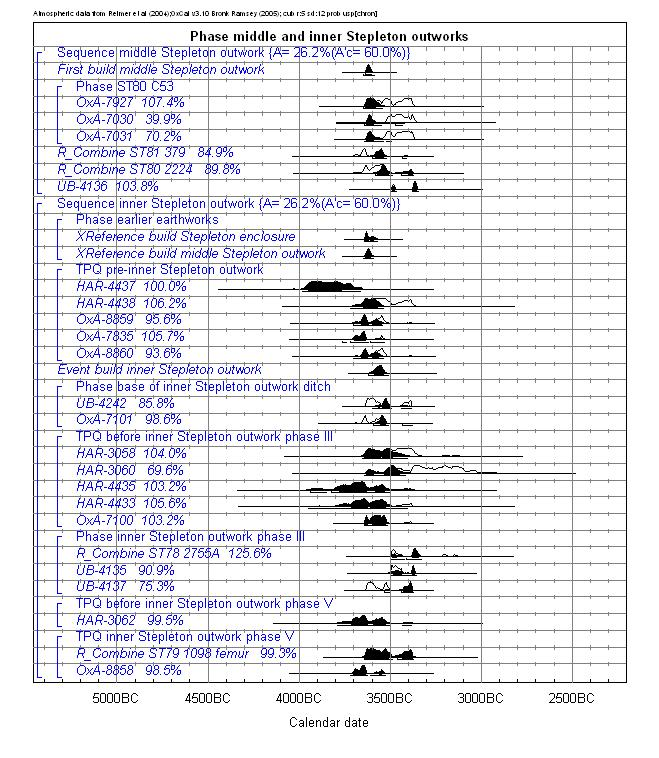
\includegraphics[width=0.7\textwidth]{figures/model5}
	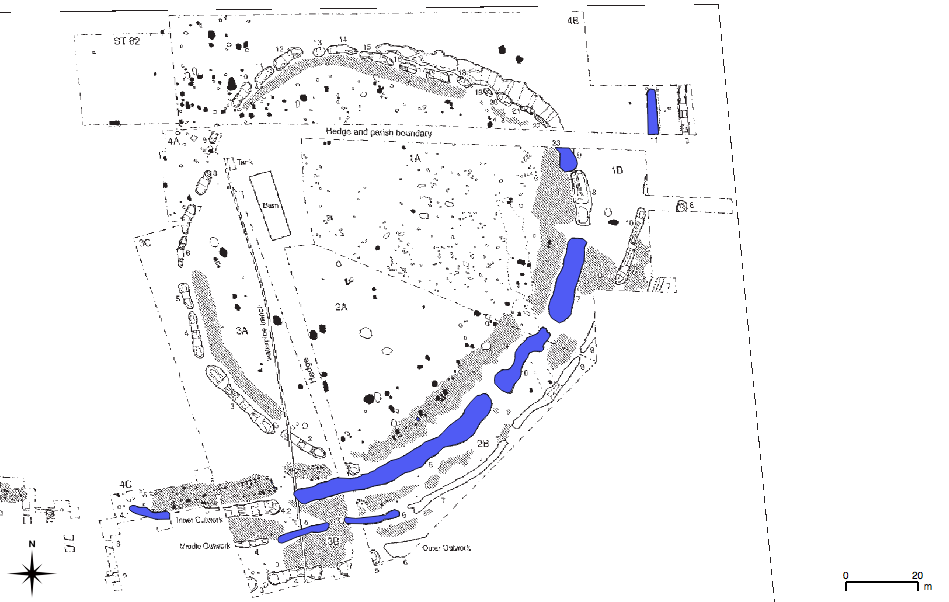
\includegraphics[width=0.9\textwidth]{figures/model5-plan}
  \caption{Bayesian model for the middle and inner Stepleton outworks and plan of the features dated, from fig 4.12 \citep[143]{Whittle:2011kl}}
  \label{fig:stepleton2}
\end{figure}

From phase I of the middle outwork come three dates on single fragments of short life charcoal taken from the base of segment six (OxA-7030, OxA-7031 and OxA-7927) that the original report concluded were homogenous and freshly deposited on the basis of a lack of significant statistical difference \cite[395]{Mercer:2008fk}. There were no phase II samples from segment six, but one from segment five (OxA-7024 and OxA-7025) and one from segment 11, (OxA-7035 and OxA-7036) both articulating. Phase III is dated by one sample from segment six (UB-4136) an articulating cattle vertebra from rubble fills \cite[395]{Mercer:2008fk}. In the original report, the authors mention that OxA-7030 has a low index of agreement at 41.8\% (but 40.4\% in the model from \citealp{Whittle:2011kl}) which they put down to an artefact of statistical scatter \cite[395]{Mercer:2008fk}. It could also be a by product of assuming that segments five, six and 11 are synchronous, as the dates from five and 11 above OxA-7030 could lead to a low agreement value if they were not strictly following OxA-7030. The approximate locations of all these dates are shown in figure~\ref{fig:pre-outwork}.

\begin{figure}
\begin{center}
	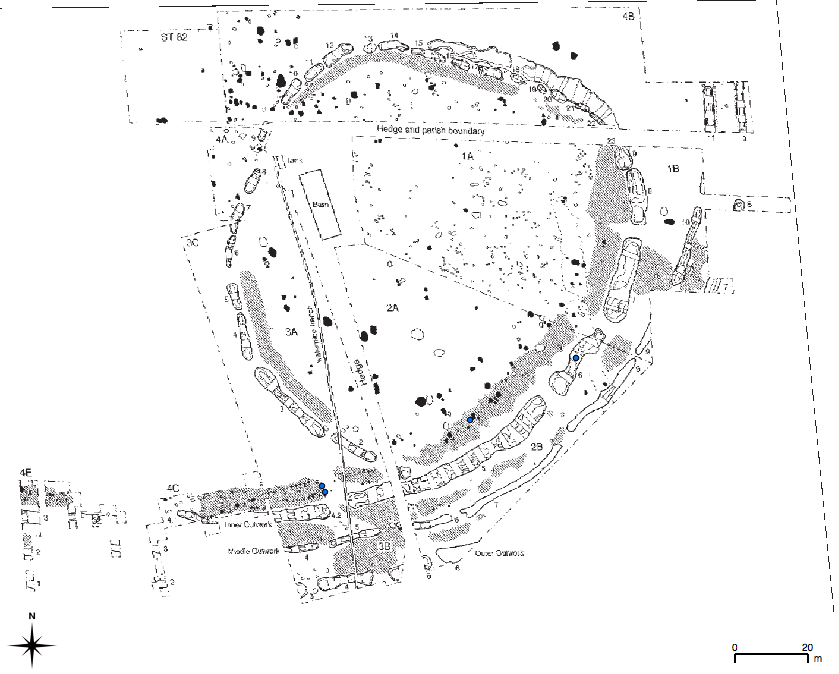
\includegraphics[width=0.9\textwidth]{figures/stepleton-preoutwork}
\end{center}
  \caption{Plot of locations of dates preceding the inner Stepleton outwork}
  \label{fig:pre-outwork}
\end{figure}

Turning to the inner outwork, the model shown in figure~\ref{fig:stepleton2} clearly shows that two sets of dates are included which pre-date the outworks construction. At the very bottom are references to other sections of the overall model, first the building of the middle outwork, and then the building of the Stepleton enclosure. The first relationship was based on the result of excavation evidence, and the second from air photographic evidence \cite[395]{Mercer:2008fk}. Following this is a set of five dates, HAR-4437 and HAR-4438 are from features situated on the enclosure side of segment 4.2, in a location at the end of the bank. These samples are from charcoal of posts burnt in-situ in the gateway \cite[395]{Mercer:2008fk}. The next date, OxA-7835 is from the bank behind segment five, this is from a sample of an articulated burial, which in the original report is assumed to have been buried under the bank \cite[395]{Mercer:2008fk}. And OxA-8859 and OxA-8860 two charcoal samples from the surface of the primary silt of segment six, which the original investigators assumed to be a part of the rampart breastwork \cite[395]{Mercer:2008fk}. This last date is considered to pre-date the construction of the outwork, as the building of the outwork followed the burning of the enclosure. As can be seen in figure~\ref{fig:pre-outwork} these dates stretch along only a part of the inner outwork, from segment six to segment 4.2. 

From phase I of the inner outwork, two dates are included in the model. UB-4242 from segment seven and OxA-7101 from segment nine. These were both from articulated burials laying on the ditch bottom  \cite[395]{Mercer:2008fk}. Following this in the model is a set of samples from various charcoal fragments, which are included as a terminus post quem as they may have derived from an earlier event \cite[395]{Mercer:2008fk}. HAR-3058 and HAR-3060 were from segment seven, HAR-4435 from segment four and HAR-4433 from segment five. Also included in this grouping of the model is OxA-7100 from segment seven, a sample from an adult skeleton, which may have been redeposited \cite[396]{Mercer:2008fk}. There were no samples from phase II, from phase III there are four samples from articulating remains in three segments, UB-4137 from segment six, UB-4135 from segment five, OxA-7044 and OxA-7045 from segment seven. These samples are statistically significantly different, in the original report this is put down to the rubble fills taking time to accumulate, based on the irregularity of the fill, and the varying locations in the fill that the different samples came from \cite[395]{Mercer:2008fk}. It could, of course, also be related to the samples coming from three different segments, lacking a homogeneity across all three in the formation of this fill. HAR-3062 from segment seven is then modelled singly as a terminus post quem, this is a charcoal sample, which as with the others may related to an earlier event. Finally, there are three samples from segment five, (OxA-7026, OxA-7059 and OxA-8858) coming from a dump of sheep remains, which the investigators believed to have been redeposited \cite[396]{Mercer:2008fk}. There is a sequence of six dates through segment seven, one from segment six, five from segment five, one from segment four and one from segment nine. However looking at figure~\ref{fig:stepleton2}, it is clear that segment five is particularly long, and the samples could have occurred anywhere along it's length. The other segments are fairly regular, with six and seven being about the same length, as are four and nine. The agreement measurement from the samples is used in the original report to suggest a common history of construction across the segments, \cite[396]{Mercer:2008fk} but there seems to be a certain circularity of argument around this, as the agreement values have been used to define the model. It would be more valuable if there was physical evidence of a common history of construction.

\subsubsection{Hanford Outworks, Shroton Spur Outworks and discrete central area features}

\begin{figure}
\centering
	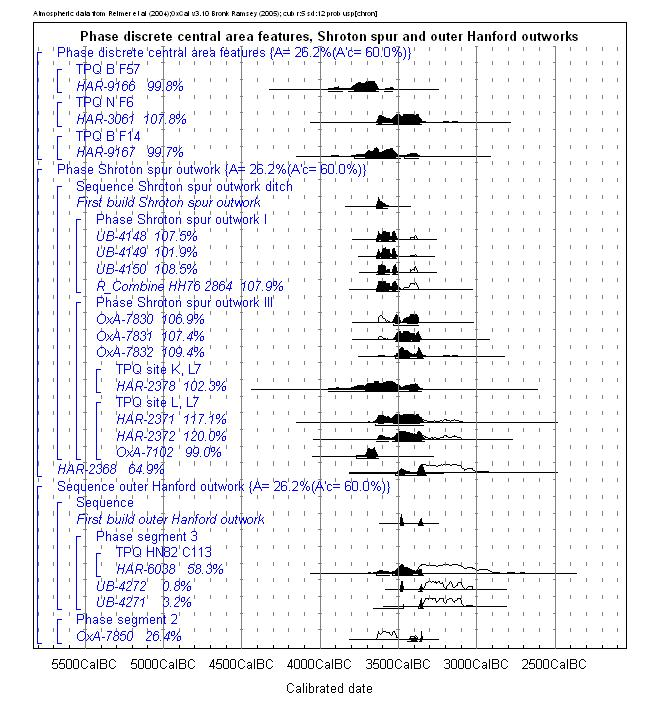
\includegraphics[width=0.7\textwidth]{figures/model6}
	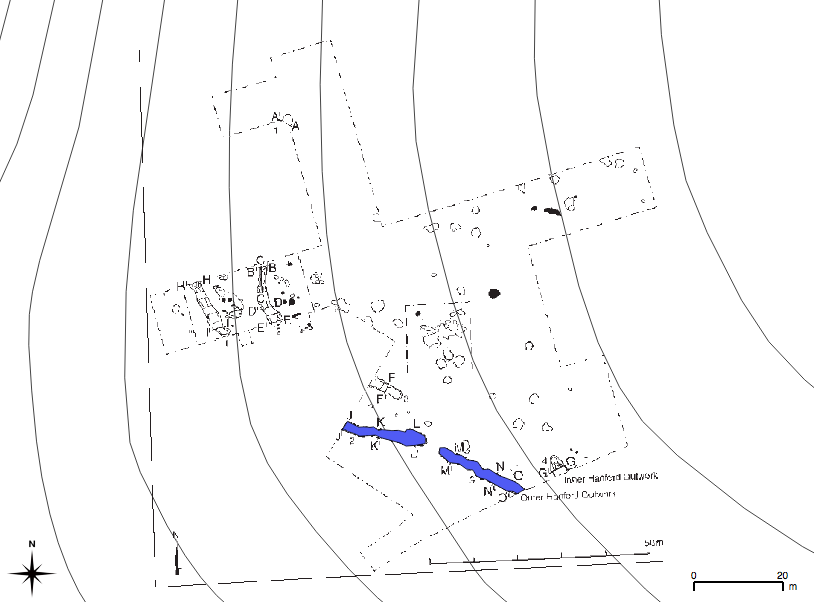
\includegraphics[width=0.9\textwidth]{figures/model6-plan3}
  \caption{Bayesian model for the Hanford outworks, Shroton spur outworks and discrete central area features; and plans of the features dated in the Hanford outwork, from fig 4.13 \citep[144]{Whittle:2011kl}}
  \label{fig:hanfordetc}
\end{figure}

This final section of the bayesian model includes several spatially distinct areas, the Hanford outworks, the Shroton spur outworks and a set of discrete features in the central area.

\begin{figure}
\centering
	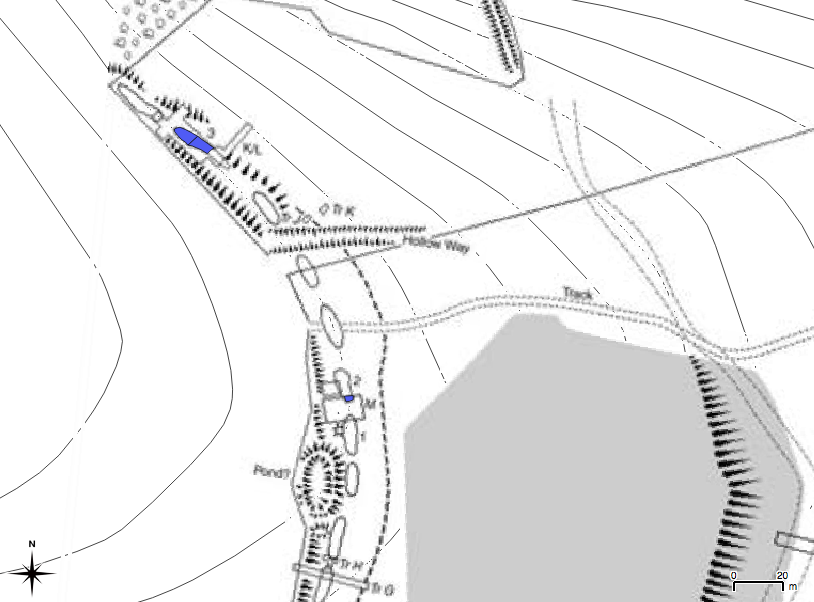
\includegraphics[width=0.8\textwidth]{figures/model6-plan1}
	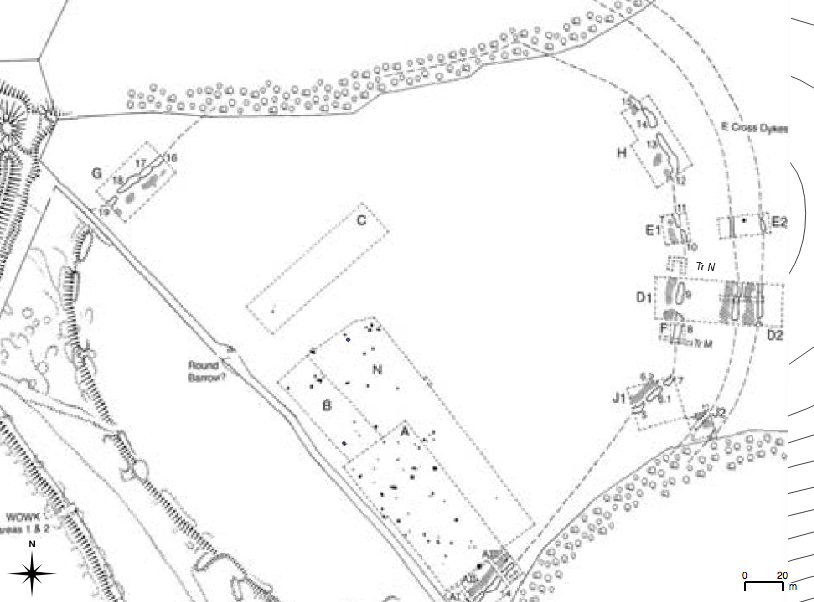
\includegraphics[width=0.8\textwidth]{figures/model6-plan2}
  \caption{Plan of features shown in the model of figure~\ref{fig:hanfordetc} for the Shroton spur outworks and discrete central area}
  \label{fig:hanfordetc2}
\end{figure}

There are a total of four dates from the Hanford outworks, three of which come from segment three, and one from segment two. Of those from segment three, one from charcoal found at the north butt, (HAR-6038) is treated as a terminus post quem as it may pre date the construction \cite[396]{Mercer:2008fk}. The other two are from articulated cattle bone found at the south butt (UB-4271 and UB-4272) that the original report concludes are likely to be very close to the construction date  \cite[397]{Mercer:2008fk}. The date from segment two comes from an articulating sample found at the south butt (OxA-7850) which was significantly earlier in date than those from segment three. The original report suggested three potential explanations for this disparity; that the samples from segment two were redeposited, that segment three underwent a ``radical'' cleaning-out, or that they were built at different dates \cite[397]{Mercer:2008fk}.

Moving next to the Shroton spur outwork, the model in figure~\ref{fig:hanfordetc} shows five samples for phase I, these all come from segment three in site K/L \cite[397]{Mercer:2008fk}. There are no dates from phase II, phase III has dates from both sites. From segment two in site M, are two dates on articulating animal bones, (OxA-7031 and OxA-7032) the rest of the dates in this part of the model come from segment three. This includes an articulating dog skeleton, (OxA-7830) human foot and toe bones (OxA-7102) which may have been redeposited \cite[397]{Mercer:2008fk} and so are treated as a terminus post quem, and several bulked charcoal samples (HAR-2371, HAR-2371 and HAR-2378). Finally there is HAR-2368, which is charcoal from a posthole of a possible gateway that the original investigators believed post-dated the ditch construction \cite[398]{Mercer:2008fk}.

Finally for this section of the model are discrete features of the central area. This is made up of three samples of bulk charcoal, including oak. Because of this they are all treated as terminus post quem \cite[402]{Mercer:2008fk}.

\section{Problems with the chronological evidence and interpretation}
A key argument for the use of bayesian modelling, and in fact many other computational techniques, is that they force us to make our assumptions explicit. In this case, by coding a model which encapsulates those assumptions. But the use of bayesian modelling on Hambledon relies on some other, much more implicit assumptions. Firstly, most of the models group dates from multiple parts of the site, sometimes just nearby segments, but also from separate areas of excavation. This relies on the assumption that the phases used to group those dates are in fact contemporary. It also assumes that the dates we do have are in a sense independent observations on the phase being dated, however this is clearly not the case. In many areas multiple dates are taken from the same context, and yield very similar results, clearly material found spatially and contextually close is often temporally close as well. There are a small number of times when this has not been the case, and such outliers are then often modelled as redeposited, so do not add much to the model. While such correlation may seem obvious, it is largely obfuscated in the current bayesian model where dates from, for example, multiple ditch segments are combined. The lack of clearly recorded find spots also makes the investigation of this type of pattern in the data more difficult and less exact. Fundamentally this will lead to those contexts that have been dated more providing greater influence over the bayesian model, and the subsequent interpretation of the site, than those which have less dates (and infinitely more than those with none). There is likely to be spatio-temporal autocorrelation within the data, due to local affects, for example, of deposition, taphonomic processes or excavation. This raises the question, how appropriate is it to combine data across parts of the site (subject to their own local affects) within the bayesian model? Secondly, the dates provided by the bayesian model are not large in number, but they have been used to provide dates for the whole series of earthworks across the site, in their entirety, clearly this is based on a similar assumption, that undated areas must also follow the same sequence of phases, occurring at the same time as those in the excavated areas. While the reliance on these assumptions may be required in order to provide a best effort temporal model of the data, they should be made explicit, as otherwise there is a risk of over using the data to draw inferences, about areas of the site that it cannot support.

\subsection{The Central Area}
The central area is the part of the site with the greatest quantity of dating evidence, the models shown in figure~\ref{fig:central1} and figure~\ref{fig:central2} are split by segments, although apart from segment nine, these are in two groups. Segments five to seven form one group, and segments 16 to 19 form the other. These two groupings are of a series of adjacent ditch segments, and so, if the physical evidence of the fills that make up the different phases supports them being combined, effectively into one segment (for the purposes of the model) this is not particularly controversial. However in some cases this may not be accurate, for example while the stratigraphy segments 17 and 18 is very similar, the dates may tell a different story. The date of an articulating sample, UB-4269, is significantly later than dates from the same phase of fills (phase III) from segment 17 (OxA-7022, OxA-7023, OxA-7099). The original report puts this down to UB-4269 being in an undetected re-cut, but also raises the possibility that the sequences were not contemporary \cite[399]{Mercer:2008fk}. 

The grouping of dates for segment five to seven only contains dates for phase I, while the grouping for segments 16 to 19 contains a deeper chronology. More problematic, perhaps is the comparison of one side of the circuit to another, a visual inspection of the original model and resultant dates could be a starting point, but unfortunately the scales used for both sections of the models are different, making this more problematic, although it would appear for example that the phase I dates for segments 16 to 19 are possibly slightly earlier than those on the other side of the circuit. When we consider their location, on opposite sides of the circuit, this would make sense, what is more surprising is that this appears to have been omitted in the original analysis of the chronology.  In order to further investigate this point figure~\ref{fig:central-phasei-model} has been generated from the original data. This shows the start boundaries for each of the segments, or groups of segments from the central area, as grouped in the original model. Once on a standard scale, it is possible to easily compare the start dates form ditch segments on either side of the circuit. Clearly the main peak of the three distributions is broadly similar, with that for segments five to seven being the most constricted, while segment nine has a broader probability, and segments 16-19 being in between the two, in terms of size of date range. The peaks in probability for segment nine and segments 16-19 are slightly later than that for segments five to seven. In terms of dates the start of segments five to seven boundary is modelled at 3660 B.C. to 3630 B.C. (68.2\%) and 3680 B.C. to 3570 B.C. (95.4\%), segment nine is 3650 B.C. to 3540 B.C. (68.2\%) and 3660 B.C. to 3530 B.C. (95.4\%), and segments 16-19 is 3650 B.C. to 3595 B.C. (68.2\%) and 3655 B.C. to 3570 B.C. (95.4\%). Clearly there is a possibility that all three sections of the causeway were constructed at around the same time, however this new output from the model demonstrates this is far from certain. Interestingly this analysis brings to light that the distribution for segment nine and segments 16-19 are more similar than that for segments five to seven and segment nine, despite the close proximity of segments five to seven with segment nine, and segments 16-19 being on the other side of the circuit. This is most likely to be an artefact of the underlying uncertainty, rather than evidence for sequencing to the ditches initial construction, as there is still significant overlap between all three, especially at the 95.4\% confidence interval.
There is very little further comparison that can be done between the north-west and south-east sides of the enclosure as so few phases are dated for both sets of segments. Phase III is a possibility, but there is very little after that from segment nine, on the south-east side, where as to the north-west there are several dates for phase IV and VI.

\begin{figure}
\centering
	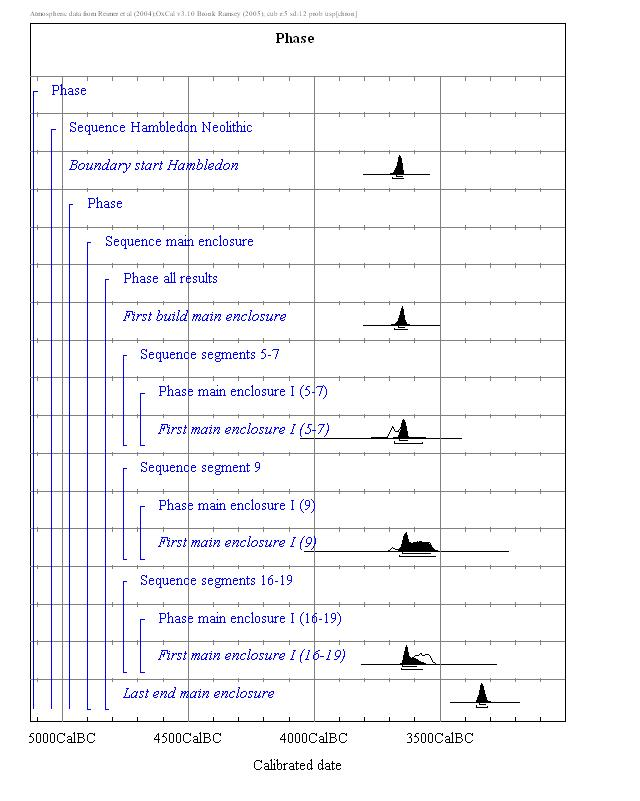
\includegraphics[width=0.9\textwidth]{figures/central-phasei-model}
  \caption{Posterior density estimates for the start of phase I in the ditch segments of the central area of Hambledon Hill}
  \label{fig:central-phasei-model}
\end{figure}

\subsection{Cross Dykes and the Long Barrow}
The cross-dykes are a prime example of a very different problem, a simple lack of data. The outer east cross-dyke only provides one date to the bayesian model, one which has been argued could come from an extension \citep[401]{Mercer:2008fk}. All that can be stated with any confidence is that after this date, segment E2 of the outer east cross dyke existed. The inner east cross-dyke is a little better, all of the dating evidence is for the first phase, so the model provides a clear date of initial construction of the cross dyke, or at least of segment four, where four out of five dates came from. It would appear that these dates are ever so slightly earlier than those for the initial construction of the central area, but this is not noted in the earlier studies. A complete lack of modelled dating evidence for any subsequent activity on the east cross-dykes means it is not possible to make any more temporal comparisons with the central area. 

The south cross-dyke suffers in much the same way, here there are dates preceding the construction, and dates of later recut activity, but nothing to date the original cutting of the ditch. An estimate for cross-dyke construction is obtained via the model, however this ignores the fact that the pre cross-dyke activity was towards its western end, whereas the later activity was more central. It assumes that construction of the cross-dyke was a fairly rapid event, rapid enough that the later recuts must have taken place after the cross-dyke had been constructed along its full length to the west. 

The south long barrow is a different case, the excavated quadrants are all close by or adjacent to one another, and there are a fair number of dates, particularly for phase I. Like the central area, the dates for phase I, and the sequence for the barrow assume that phases are comparable across the quadrants. In this case that would seem to be a fairly likely scenario, although it is possible that different sides of the barrow may have been cleared at different times. As the dates for phase I all came from one quadrant and the dates for phase II, III and IV all came from another different quadrant, and the excavation report contains no indication of a synchronous sequence, there is no clear dating evidence either way. 

\subsection{The Stepleton Enclosure}
The model for the Stepleton enclosure and outworks is very different to that for the central area, this model is not separated out by ditch segment, meaning its accuracy relies on the sequences of its segments being synchronous. Unfortunately, the excavators could not be sure that this was the case \cite[394]{Mercer:2008fk}. Part of the problem is the lack of dating evidence for each phase, and the lack of sequences of dates in any segment. The result is a sparse model that combines data, where there is a clear lack of evidence that the data should be being combined. The phase I section of the model contains samples only from segment three, so we can be confident that these provide a date around the time of its construction, but there are no dates for the construction of any other segments. So to assume that the date from the model for `first build Stepleton enclosure' is applicable to the enclosure in its entirety is, at best, optimistic. The discrete features in and near to the enclosure are included in the model, but as they are included in a phase they have little to no effect on the overall model, and only act on other dates within their phase. 

The outer Stepleton outwork has only one date, which provides a broad potential range for the digging of the butt of one segment. The middle outwork suffers the same problem as the enclosure, in that a sequence of dates is built up from dates coming from multiple segments, the results of which are extrapolated across the whole outwork. There are also very few dates, for example for phase III there is only one. The inner Stepleton outwork has a greater number of dates, but does suffer from the same issue of combining dates from multiple segments in the same part of the model, in this case five segments. The reference to the middle outwork, which is modelled as earlier than the inner outwork is, in fact, modelling that segment six of the middle outwork pre-dates a set of pits, which are in fact not in its vicinity, or near the closest section of the inner outwork. In particular, the samples for phase III were statistically significantly different \cite[395]{Mercer:2008fk} which may be down to the slow rate of accumulation of the fills, or it may be that the four samples came from three segments, which did not have a synchronous sequence. This is clear evidence that the spatial locations for the source of dates in bayesian models should be considered, as this does offer an alternative explanation to the one from the original report.

\subsection{The Hanford Outworks}
The plan for the Hanford outworks suggests a significant part of it has been dated, unfortunately the dating evidence is very thin. The dates are separated by ditch segment, but all the dates would appear to come from close to the base of the ditch, so there is no sequence as such, assuming the segments are contemporary. The date taken for the initial building of the outworks is almost solely influenced by the two dates from the south end of segment three. With the terminus post quem from the north end of segment three and the date for segment two having little impact on the first build date, even though the date for segment two is significantly earlier. The model in this case appears to be reflecting one of the original reports interpretations of this earlier date, that the dated material in segment two is redeposited. While the three potential interpretations have clearly considered the spatial evidence, in so far as they suggest the two segments might have had different use lives, either one being much more recent, or the other having had a substantial clean out. These segments are very close, which would make it seem less likely they had such different use lives, however the plan in figure~\ref{fig:hanfordetc} does show that the two segments are on substantially different alignments. This evidence would favour the suggestion that segment three was a later addition to the outworks. However when an alternative version of the model was run, as shown in figure~\ref{fig:hanford-remodelled}, with the sequence for segment three included inside another sequence, to indicate a strict ordering following segment two, the agreement index values fall so low that clearly with the evidence we have, such a strict ordering is not supported. For example UB-4272 falls down to 0.9\% from 61.6\% in the original model. A clear benefit to the bayesian modelling approach is that it allows for such experimentation and the construction of alternative versions of reality. In this case, we can rule out (based on current evidence) one such potential version of events, and must assume instead that either the sample from segment two was redeposited, or segment three underwent a radical clear out.

\begin{figure}
\centering
	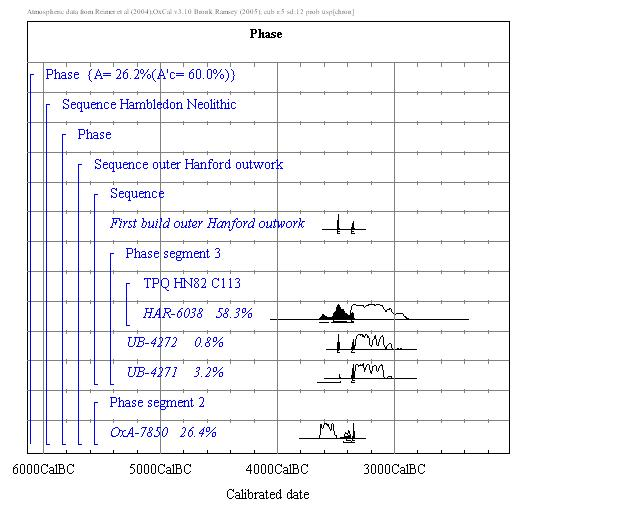
\includegraphics[width=0.9\textwidth]{figures/hanford-remodelled}
  \caption{Posterior density estimates for an alternative model of the Hanford outworks, where segment two pre-dates segment three.}
  \label{fig:hanford-remodelled}
\end{figure}

\subsection{The Shroton Spur Outwork}
The Shroton spur outwork model takes dates from two excavation areas, and as with other models, combines them into one component of a sequence block, assuming that the phases are comparable. And the computed first build date, calculated from only a very small part of the outwork, is assumed to be representative of it as a whole. While the dates may show a good agreement index when placed in the model in this way, the model should ultimately be guided by the archaeology, and not the computed agreement index. The dating evidence for the Shroton spur is ultimately a sequence of the earliest phases from a single ditch segment, plus two corroborating dates from similar fills in another segment. This is not really enough to suggest a unified construction, and lacks dating evidence from any later activity.

\begin{figure}
\begin{center}
	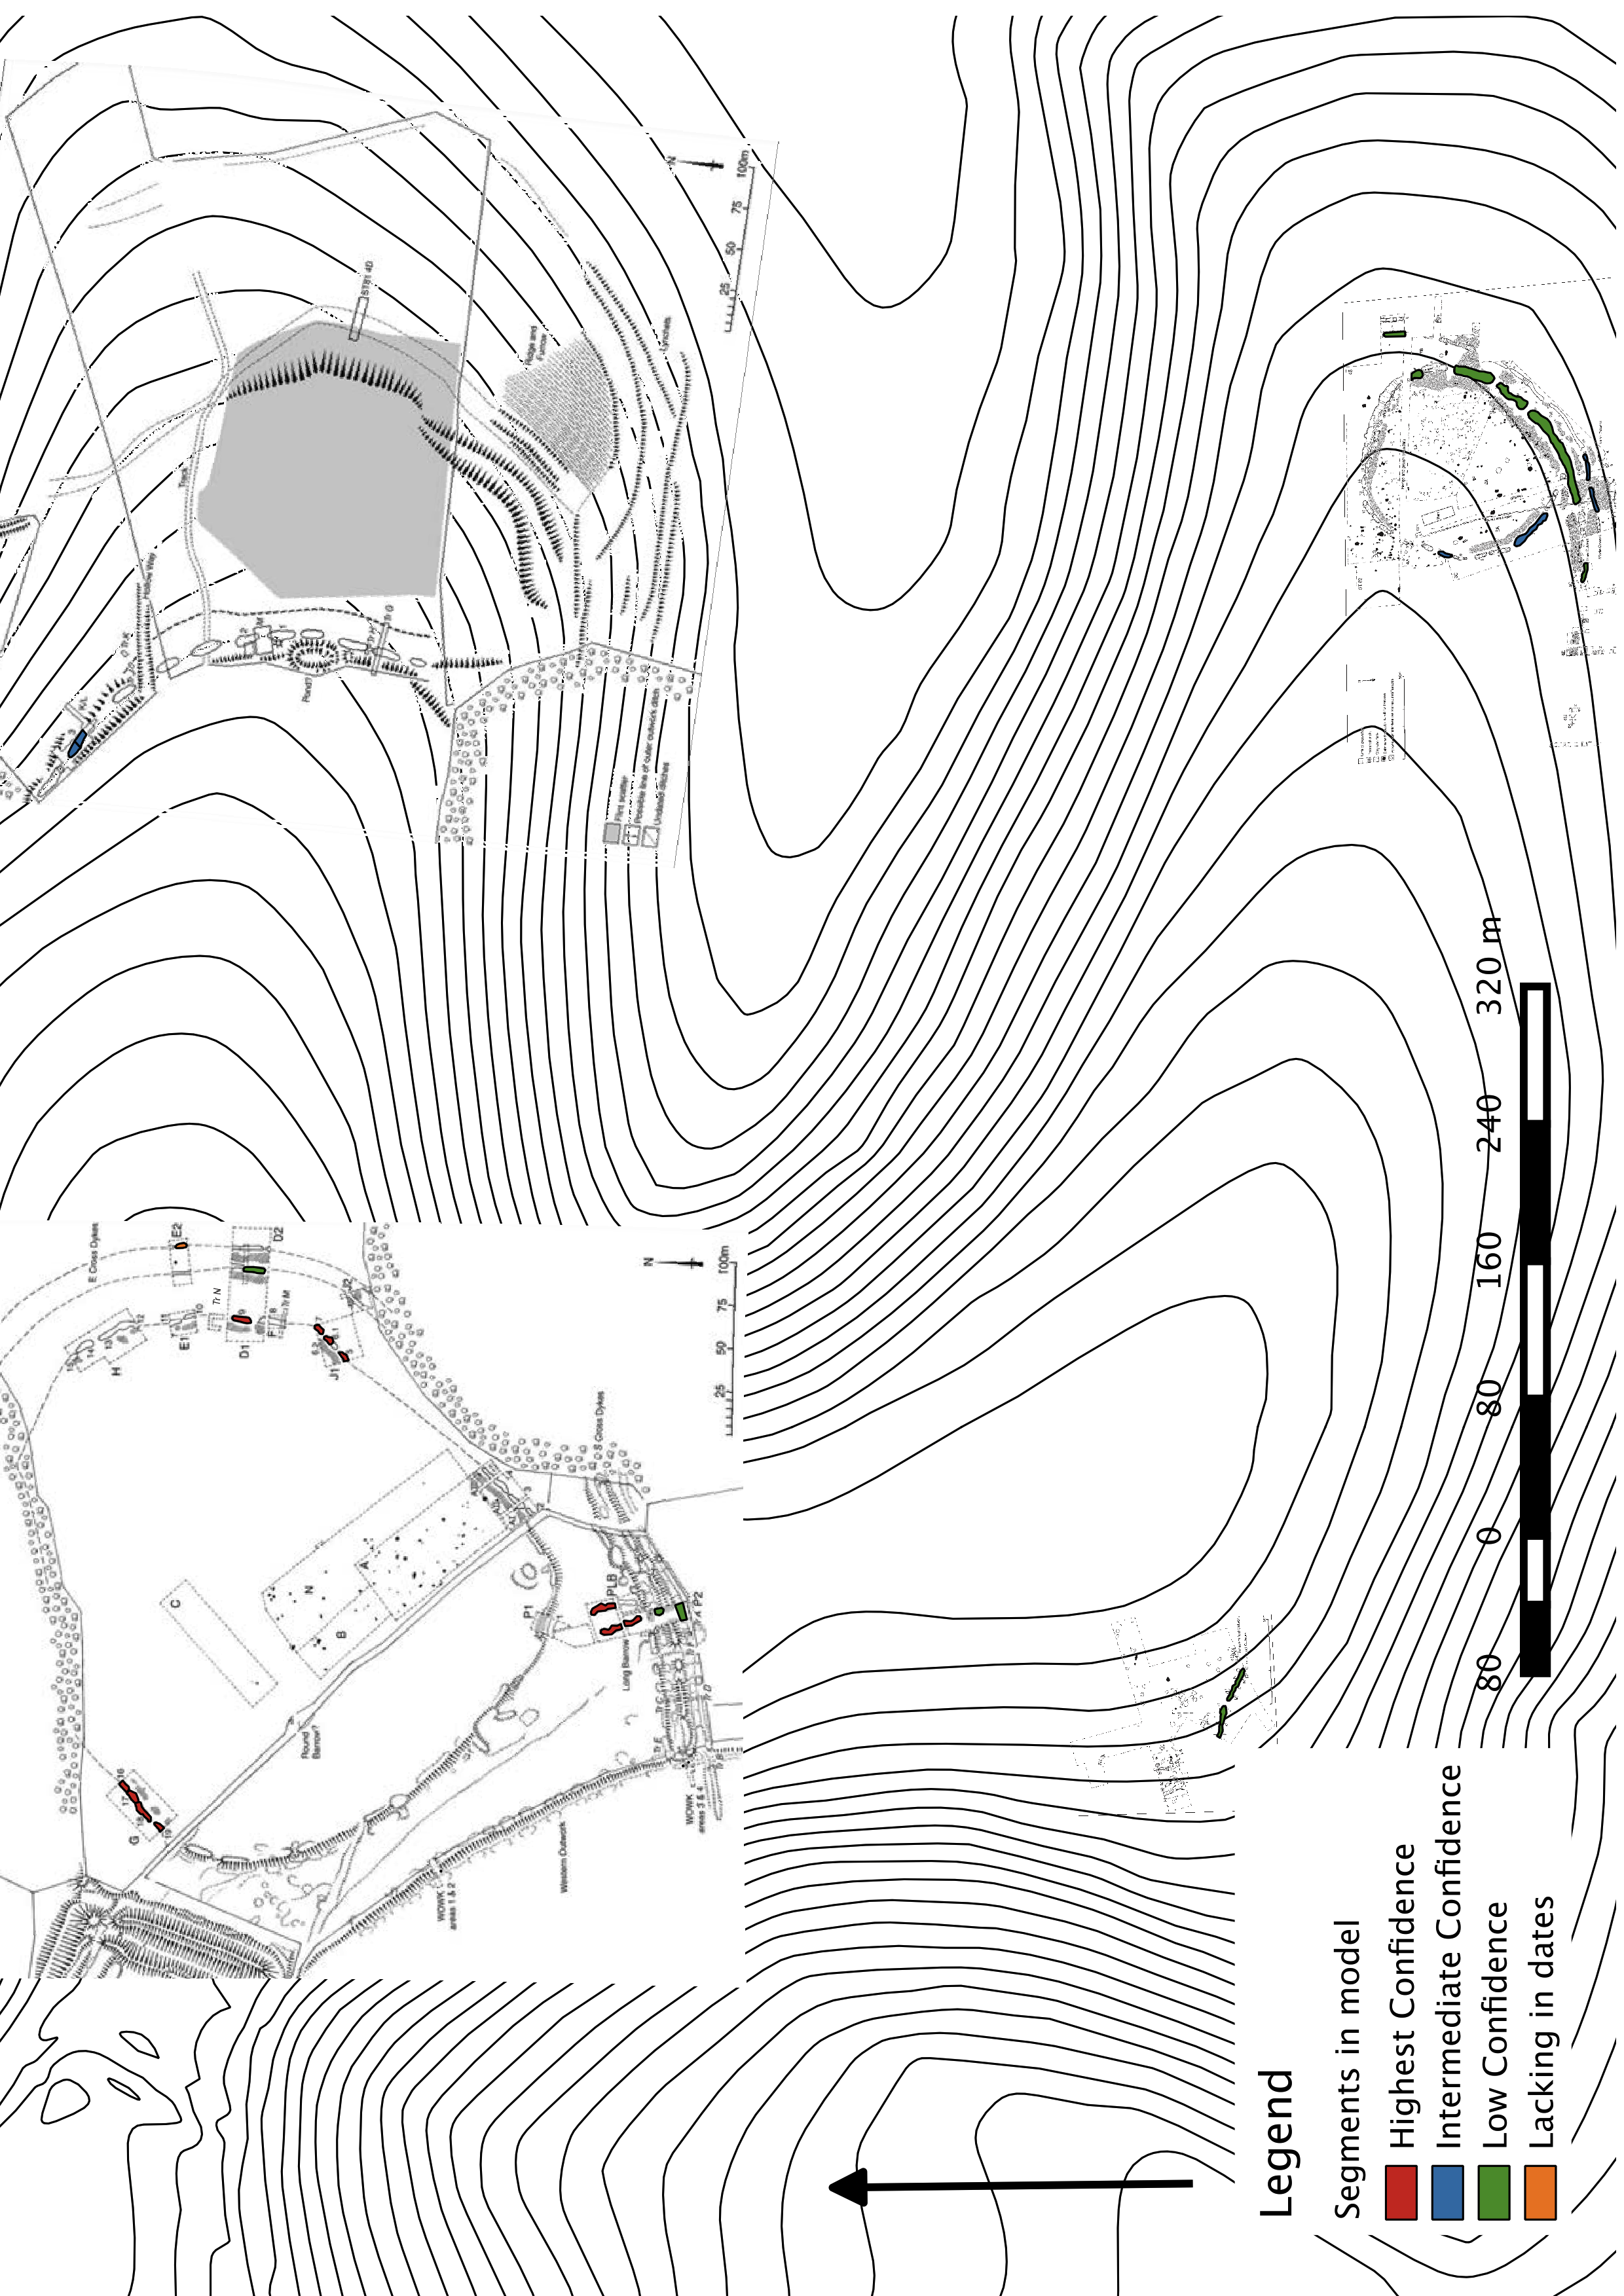
\includegraphics[width=0.9\textwidth]{figures/dated-confidence}
\end{center}
  \caption{Plan of segments included in the bayesian model, by qualitative confidence interval}
  \label{fig:dated-confidence}
\end{figure}

\subsection{Confidence in the interpretation}
In conclusion, the chronological evidence varies across the site; in some areas the models more accurately reflect the spatial nature of the evidence, while in others dates from relatively distant segments are combined as though they were found side-by-side. Clearly the kind of joint spatial and temporal model display, as shown above, aids the spatio-temporal interpretation of the evidence, enabling the archaeologist to easily assess whether there may be spatial issues with a bayesian model. The review above has also shown that a bayesian model does not capture all of the uncertainty around a defined chronological model of the archaeology. Additional key uncertainties around the comparability of phases remain implicit, as does the applicability of a model across un-excavated areas. 

It is possible to rank the confidence of the model across various parts of the site, based on the descriptions above. Such a ranking is clearly qualitative. The areas falling into the highest confidence bracket have a set of dates for a particular segment modelled in a chronological order,  in this case only the central area fits that requirement. The next group would be those dates that have one but not both of these, e.g. a set of dates in order, but from multiple segments, or a very limited number of dates from a single segment. Into this set fits: the south long barrow, Stepleton enclosure, middle Stepleton outwork and Shroton outwork. The low confidence areas those where there is some doubt over the validity model, following a consideration of the spatial evidence this group includes: the inner east cross dyke, south outworks, inner Stepleton outwork and the Hanford outworks. And the final group is those areas simply lacking in dating evidence: the outer east cross dyke, western outworks, outer Stepleton outwork and isolated pits in the central area. This grouping of segments is displayed in figure~\ref{fig:dated-confidence} and in figure~\ref{fig:dated-confidence-buffer} with a 10m buffer. 

\begin{figure}
\centering
	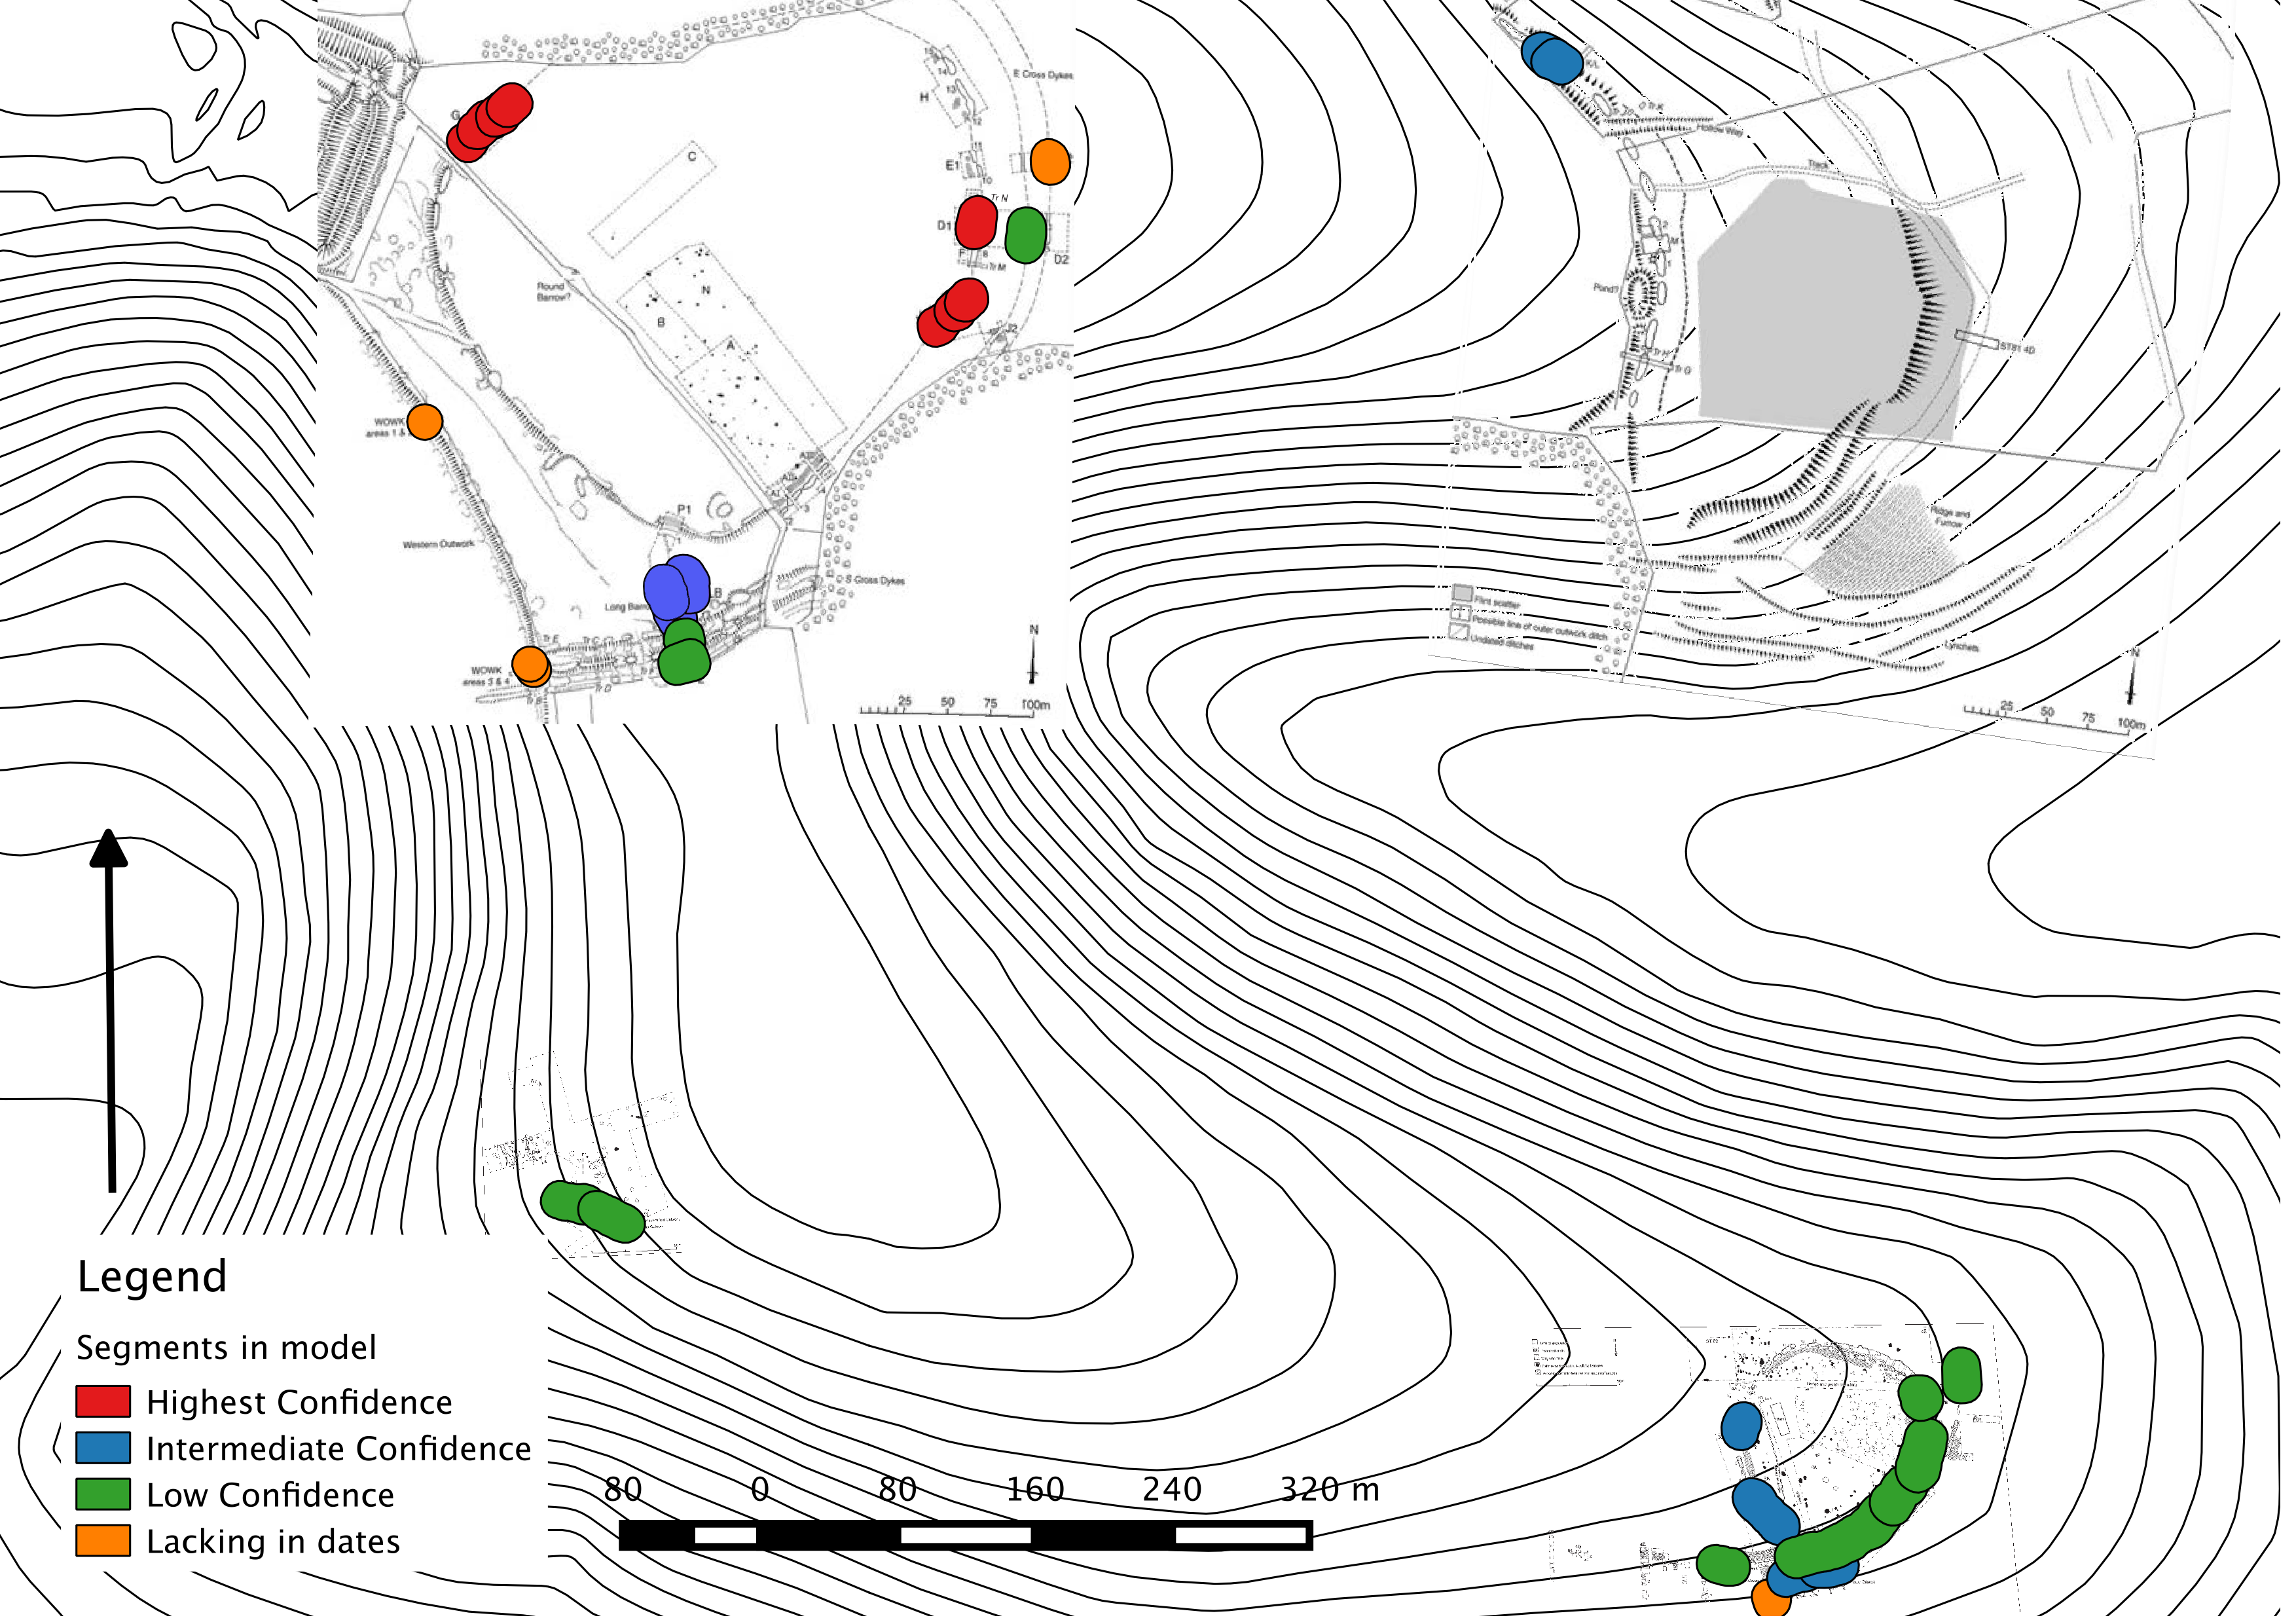
\includegraphics[width=0.9\textwidth]{figures/dated-confidence-buffer}
  \caption{Plan of segments included in the bayesian model, by qualitative confidence interval, with 10m buffer}
  \label{fig:dated-confidence-buffer}
\end{figure}

Clearly the focus for any chronological or temporal interpretation of the evidence should be focused around these areas. An arbitrary 10m has been applied for figure~\ref{fig:dated-confidence-buffer} to aid visual identification. If we accept the implicit assumptions of the bayesian model for Hambledon Hill, that un-excavated areas are likely to have the same sequence of fills as excavated, then we may consider surrounding ditch segments to take the dates from those in the bayesian model. However the extent to which this might be applicable is impossible to accurately asses without excavating those areas. For areas that have been excavated, but provided no dating evidence, if it is possible to provide evidence that the dated fills were synchronous, we can transfer the dates with some confidence, as is done in almost all of the models of Hambledon Hill. In this case the areas of assumed dates, should adopt a confidence level below that of the original area.

These limitations with the temporal evidence have all been highlighted by a combined spatio-temporal review of the data and bayesian analysis. Having reviewed such limitations in detail, the next step is to further investigate the benefits of combined spatio-temporal analysis, in particular quantitative analytical methods.

\section{Quantitative Analysis}
The spatio-temporal distribution can be further investigated using a variety of quantitative techniques to formally asses the distribution of dates from Hambledon Hill across space and time. The results of such methods must be considered carefully as they can hide a variety of complexities with the data and assumptions in the method itself. There are a wide variety of spatial statistical methods from which to choose, many of which are provided as part of modern GIS packages, however such methods are not necessarily applicable to radiocarbon dates. In order to use such standard techniques, it is necessary to approximate each bayesian modelled radiocarbon date as a single value, it is these values which will be used to compute the statistics. 

Approximating a radiocarbon date can be done in a variety of ways, for example an average, such as the mean or median; or by selecting a date at random from within the distribution, with or without weighting the choice using the dates underlying distribution; or some other esoteric method for approximating the value. In many ways this choice is arbitrary if the goal is to find the `best' approximation, as there is no way of evaluating the accuracy of the selected value. The best we can do is identify a good approximation, taking reasonable account of the underlying probability distribution.  

In order to simplify the process and focus on the methods of analysis (rather than the method of approximation) averages from the probability distribution will be used as the approximate value for the subsequent analysis. The original bayesian analysis was undertaken using version 3 of OxCal, which produces a mixture of binary and text file output. To simplify extracting the averages (as calculated by OxCal) a one time transformation was undertaken as part of this project, using the following process:
\begin{enumerate}
\item The model was extracted from the OxCal 3 project, HHall.14i file, which contained the full model
\item This model was then imported into a new OxCal 4 project 
\item The OxCal 4 project was evaluated
\item A custom script is used to extract the averages from the OxCal output .js file
\item The averages are added to the shapefile of radiocarbon sample locations
\end{enumerate}
Due to the nature of the calculation process this has resulted in some values being slightly different than the values used to up this point.

\subsection{Moran's i}
A suitable technique for this data set is Global Moran's i. As a broad measure it can provide valuable summary statistics over the whole data set, with the potential to follow up using more fine grained techniques. As a measure of spatial autocorrelation when applied to the date values over the whole study area it will generate a statistic that indicates whether like values tend to group together spatially, be distributed randomly, or to be far apart. There are a series of variable parameters for the calculation of Moran's i as implemented within ArcGIS, the first being the feature value. OxCal produces two averages, the mean and the median vaules of the calibrated date probability distribution. Due to the simplicity of extraction and calculation it seems reasonable to perform the analysis using each. The next parameter is the conceptualisation of spatial relationship, the ArcGIS documentation \protect\citep{ArcGIS:fk} states that the inverse distance methods are appropriate to model processes where the closer two features are in space, the more likely they are to interact/influence each. As we are attempting to assess the spread of sample values across the site that could be influenced by past activity, taphonomic processes, research bias and recovery methods, the assumption that closer features are more likely to interact than farther ones is fair. The next parameter is distance method, either euclidian or manhattan - euclidian was used for all analysis, as manhattan is not appropriate in this context. The distance threshold was set as the extent of the dataset, so all points would influence all other values, as there is no obvious arbitrary value which would be applicable across the site. 

The ArcGIS tool also allows customised weights to be specified as a conceptualisation of spatial relationship. Clearly there are many potential ways of using it. A relatively simple option is a boolean weight on a per feature basis, so this would mean that each date has a weight of one for all other dates from the same feature, in this case mostly pits or ditch segments, and 0 for everything else. This effectively means that all dates from the same feature heavily influence one another, compared to those between features, however it removes the spatial distance between features as a component of their relationship, it also does not consider the stratigraphic relationship.
Removing the spatial distances is not a particular problem, as the features are all fairly small in size, and the locations given within the GIS are only approximate, in fact for many of the dates the only location provided in the report is a feature name, so an equal weighting of within feature dates is not an unreasonable assumption.

\csvautolongtable[
  table head= \caption{Results of calculating Moran's i to evaluate the extent of spatial autocorrelation between each dated sample across the Hambledon complex}\label{tab:moransi} \\\hline
               \csvlinetotablerow\\\hline
               \endfirsthead\hline
               \csvlinetotablerow\\\hline
               \endhead\hline
               \endfoot,
]{figures/moransi.csv}

The results from the different combinations of averages and conceptualisations of spatial relationship are summarised in table~\ref{tab:moransi}. The crucial piece of information is provided in the conclusion column, which is that for all of the combinations the results do not appear to be significantly different to a random distribution. This is an interesting result as it has already been shown that the bayesian models have spatial issues, in particular that it is unusual for a feature or segment to provide a set of dates that are spread throughout the chronology. A good example being the central area, where most of the dates for the early phases come from one side of the enclosure, and those for later phases from the opposite side. This is likely due to two main causes, firstly the averages used hide a wide degree of variability caused by the random effects of radiocarbon dating, calibration and bayesian modelling. Secondly the dates used come from a bayesian model, they were selected to provide a depth and breadth of time, so a lack of spatial autocorrelation is an indication that the model has been well constructed. The results clearly reflect positively on the construction of the model, although clearly there are concerns that have not been identified by this statistical method, most likely due to the average being used as input data.

\subsection{Stratigraphic Distance}
The weighting or relationship values used so far have been based on spatial distance between dates. While the method has not been entirely a-temporal, the weighting between two dates has not incorporated any form of temporality. When considering a purely spatial weighting between the dates, there is no autocorrelation - the distribution of average date values is indistinguishable from random. In order to incorporate some temporality the stratigraphic distance can be used as a source for a custom conceptualisation of space. This would give dates that are stratigraphically closer to one another a greater weight than those which are stratigraphically more distant. Applied over the whole site this would remove any spatial component from the weighting, however the boolean per feature weighting can be combined, including a limited spatial component, of whether dates are from the same feature or not, in the weighting. There is no Harris matrix diagram for Hambledon Hill, which would be the obvious starting point for creating such values, this leaves the layer numbers, and associated sections as the source for stratigraphical information. Of course this stratigraphic data has already been transformed into a model for the bayesian modelling process, the bayesian model therefore can provide a source for the stratigraphic relationships between dates. While this model is an abstraction from the raw data, it also incorporates an interpretation, putting the dates in an order. It is this ordering that will be used to create a value for stratigraphic closeness. OxCal has two methods of grouping multiple dates, by sequence and by phase. Dates within the same phase are assumed to belong to events which occurred concurrently, where as sequences are events that occurred in the specified order. These can be nested, so often there will be a sequence of phases. An inverse distance approach can be used to transform this into a numerical value, where the value is the inverse of difference in the order of a sequence between two dates. Dates within a phase can be assumed to be concurrent, and so given a relationship value of one.

The depth (vertical distance) between finds was not used as different fills had different depths of content, and so this distances does not provide a reliable measure of how dates relate to one another chronologically. However neither chronological distance nor vertical distance provides a consistent and reliable measure of how far apart temporally the two samples were deposited. One possibility would be creating a combined chronological and spatial autocorrelation weight, however the reason this has not been done for Hambledon is the plotted locations of dates are estimates, in most cases it was simply the ditch segment. In other cases they were plotted on diagrams in the original report, but combining these with those where only a very rough location was available would imply a false sense of accuracy. The spatial component of the weight must be such that it can logically be combined with the stratigraphic component. Due to the fact that most of the locations are only at the level of the feature, using the exact x and y c-ordinates of the plotted locations creates a false sense of accuracy. As a result of this the most compatible representation of space is probably the boolean weight per feature, as this will asses whether the date value distribution within features, weighted by stratigraphic distance is distinguishable from random. 

\csvautolongtable[
  table head= \caption{Results of calculating Moran's i using two custom conceptualisations of distance between each dated sample across the Hambledon complex}\label{tab:moransi2} \\\hline
               \csvlinetotablerow\\\hline
               \endfirsthead\hline
               \csvlinetotablerow\\\hline
               \endhead\hline
               \endfoot,
]{figures/moransi2.csv}

The results for using a purely stratigraphic weighting and a stratigraphic weighting combined with a boolean per feature weighting are summarised in table~\ref{tab:moransi2}. The two different models demonstrate two different representations of the ``distance'' between dates. In a purely stratigraphic representation the spatial locations of the dates are not factored into the weighting of relationships between the dates. The very strong positive autocorrelation is not unexpected as it is simply stating that similar dates occur closely within the bayesian model. By augmenting this representation of distance with the spatial data the Moran's i statistic can be used to confirm the observation above, that groups of dates within the bayesian model, usually comprising a phase section, cluster spatially. 

The clustering of dates demonstrated in table~\ref{tab:moransi2} confirms the observation above, that groups of dates cluster spatially. But it does not provide any indication of the cause of that autocorrelation, It could be that the results are entirely due to the random nature of the radiocarbon method. It could be that the positive auto-correlation is down to the construction of the model, in inclusion of specific results, or the way samples were chosen to be dated. Or it could be that activity on the site clustered in certain areas, during certain times. This was the conclusion of the analysis of the bayesian model, so it would be fair to conclude that the positive auto-correlation is also the result of this. Like the bayesian model multiple models can be constructed and compared, in this case of different methods of weighting relationships between the date values. That the weighting based solely on the bayesian model showed a very strong likelihood of clustering of date values is not a surprise, this shows that those dates modelled as from the the same part of the chronology tend to have similar values, compared to those that are not stratigraphically close. Perhaps more of a surprise is that when the weighting is modelled as solely spatial the distribution is indistinguishable from a random distribution, even when using the boolean weights within feature measure, which might have been expected to have shown some evidence of clustering. 

What this means is that it is not possible to say that date values show any evidence of spatial autocorrelation, when dates from the whole duration of the sites use are included equally. Put this way, it is perhaps less of a surprise, different areas of the site will have been a locus of activity in different times, and may have gone in and out of focus (and then back in again). As the biographical approach reminds us, sites often have rich histories of use and re-use, re-interpretation and it would perhaps be naive to expect such a broad measure as Moran's i to show spatial autocorrelation of date values over a site with such a rich history. So while it might be not much of a surprise that combining a spatial model indistinguishable from random and a stratigraphic one that is very strongly clustered would lead to a less strongly clustered result, it is in fact a very important outcome. Its true significance is in demonstrating the value of combined spatial and temporal analysis, showing that across the whole site, throughout its use, date values are likely to cluster chronologically, within features. As mentioned before, this supports the observation above, that certain sections of the bayesian model's chronology come from distinct areas and very few areas provide a chronological vertical section through the model. The result of this is that sequences are built with dates for different phases coming from different features.

\subsection{Local Measures}
Clearly if there was a more accurate way to approximate the dates to a single value, this would potentially make the use of Moran's i more valuable. It is also worth considering local statistical measures as these will be more focused on a subset of the results. Two such measures, with the potential to add value are Getis-Ord Gi* and the Anselin Local Moran's i as the presence of hot spots and clusters or outliers of feature (i.e. date) values is highly likely.
 
\subsubsection{Anselin Local Moran's i}
A standard measure of local spatial association, it is included in ArcGIS as a method to generate an output feature class containing identification of clusters and outliers. Figure~\ref{fig:cluster-hh} and figure~\ref{fig:cluster-lh} show the results of running this analysis using the combined chronological and spatial custom conceptualisation of space, with boolean feature values. Using either the mean or median date values identified the same dates as clustering and outliers, so only the output for the mean is shown in the figures here.

\begin{figure} 
\centering
	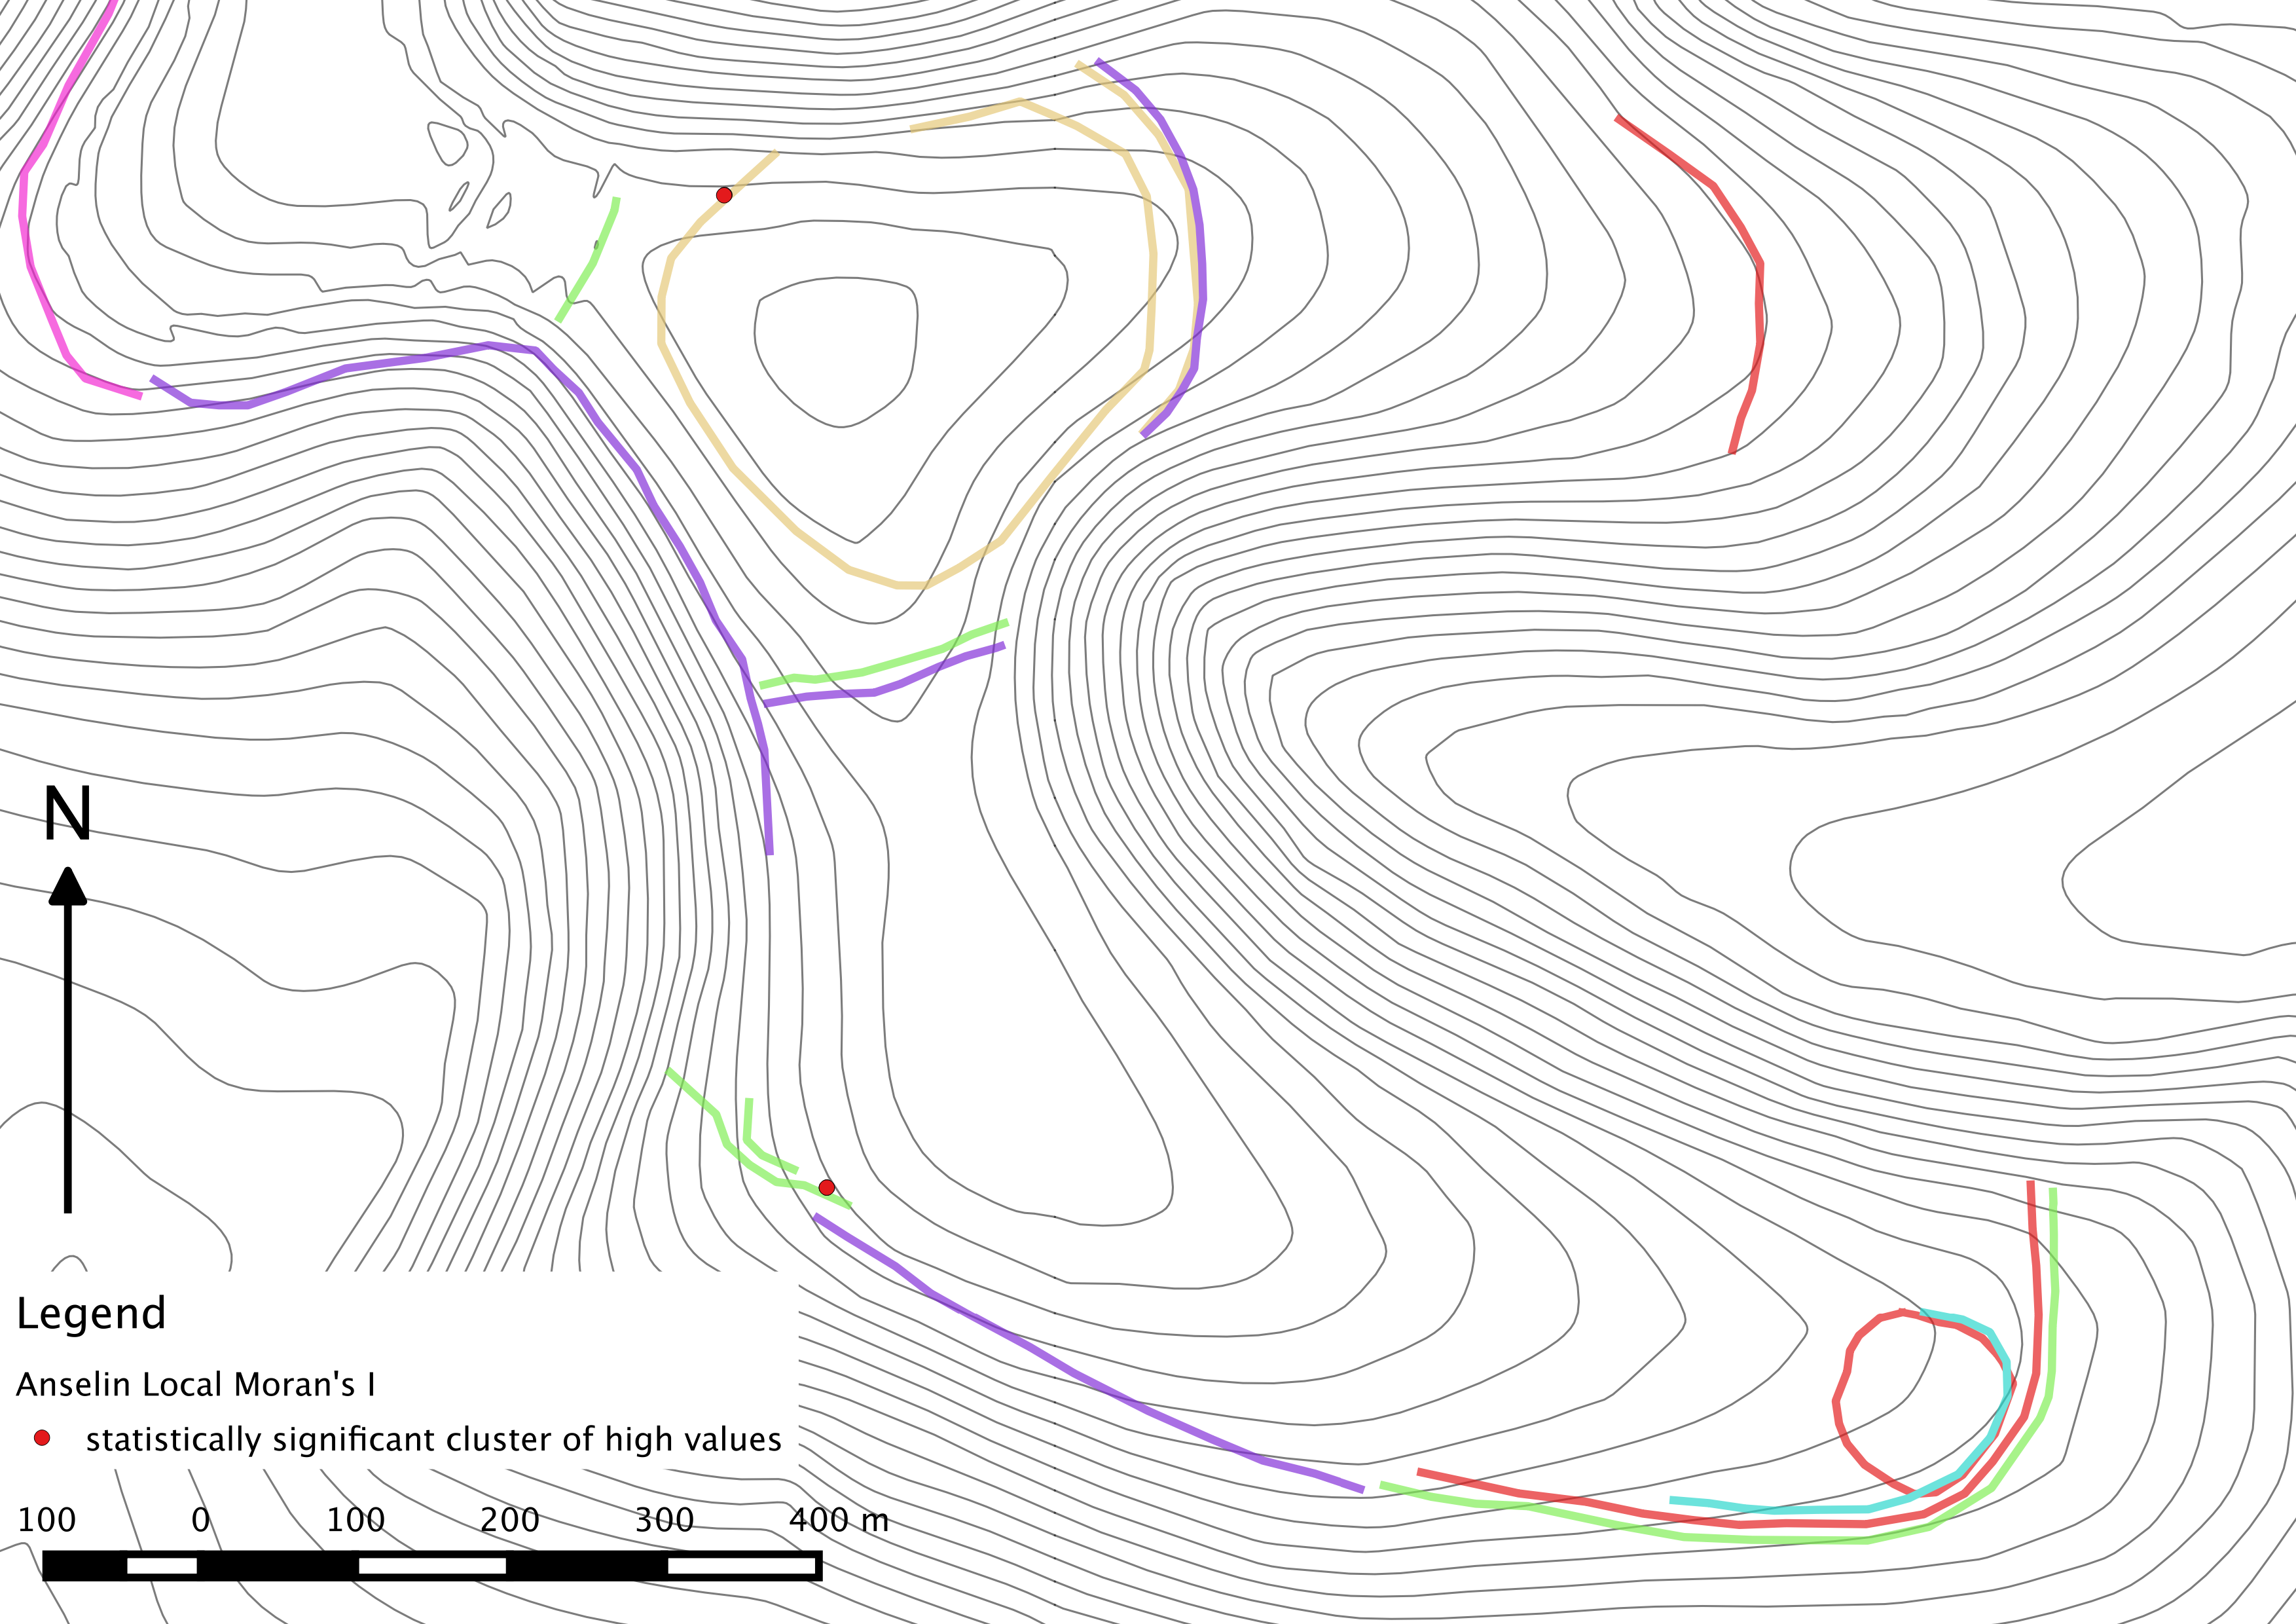
\includegraphics[width=0.9\textwidth]{figures/cluster-HH}
  \caption{Plan of statistically significant clusters of high values}
  \label{fig:cluster-hh}
\end{figure}

\begin{figure} 
\centering
	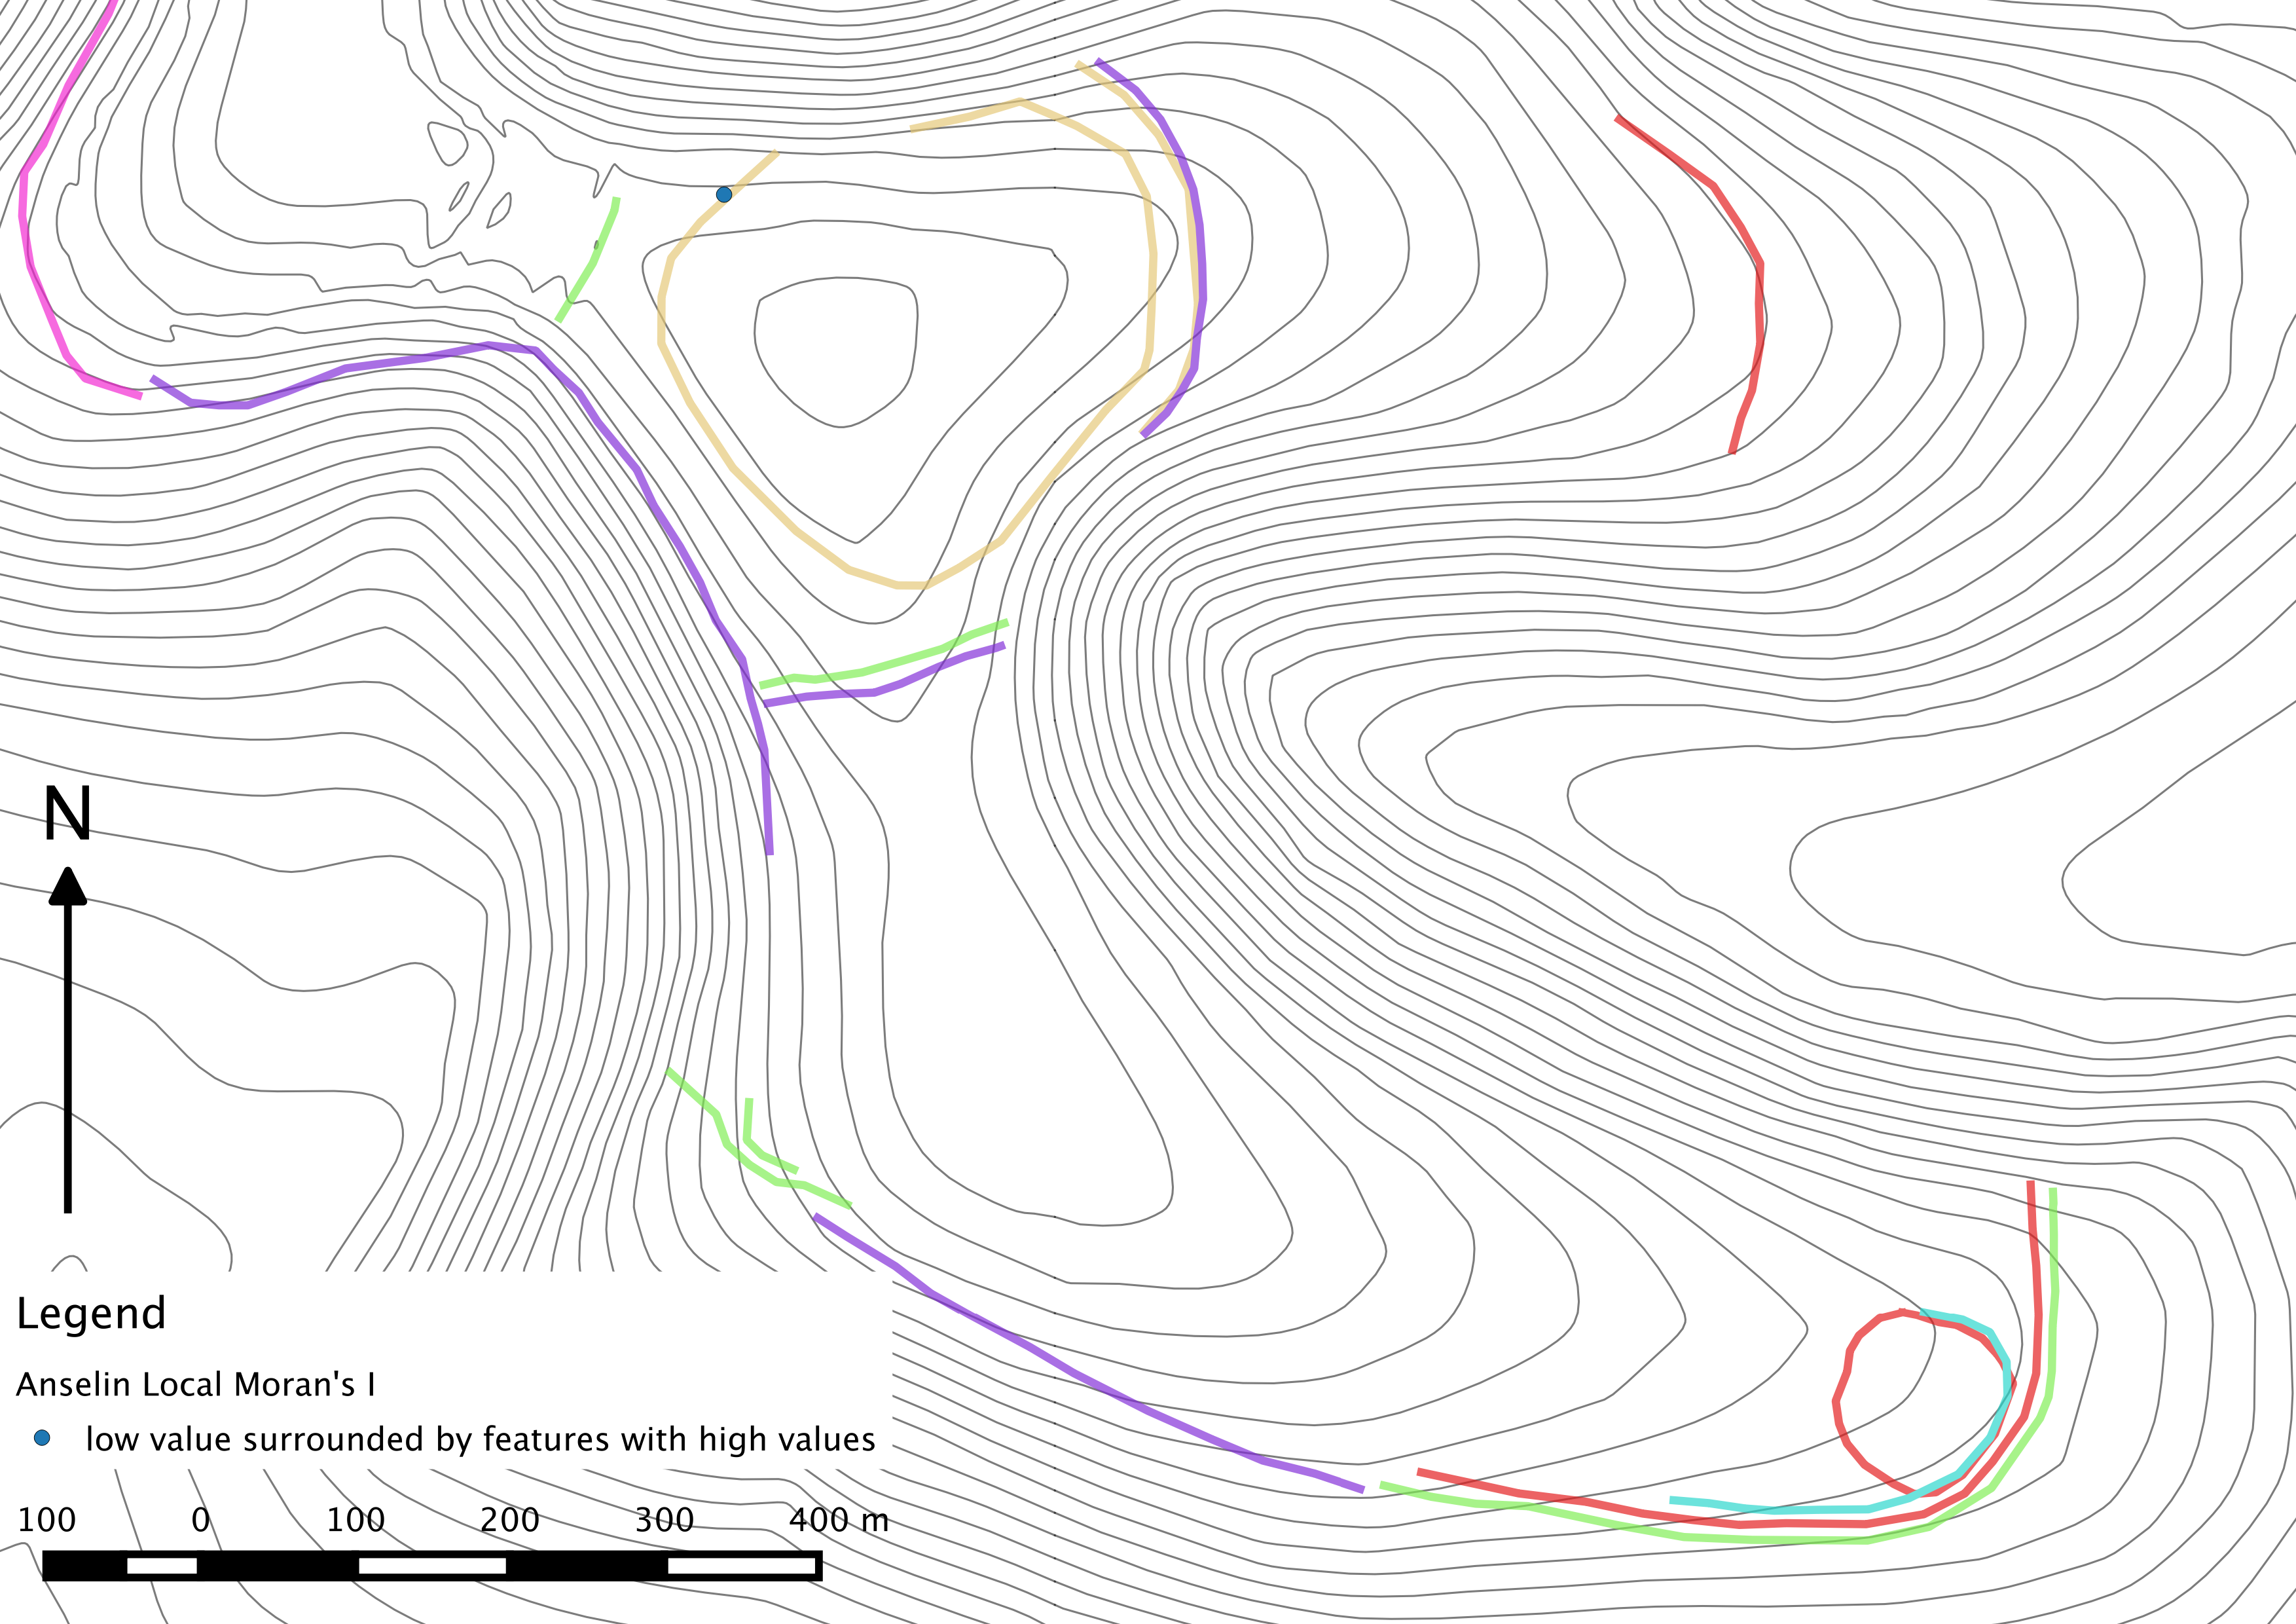
\includegraphics[width=0.9\textwidth]{figures/cluster-LH}
  \caption{Plan of statistically significant low value outliers}
  \label{fig:cluster-lh}
\end{figure}

The statistically significant clusters of high values shown in figure~\ref{fig:cluster-hh} are in two locations, the north west side of the central enclosure and the east side of the Hanford outworks. From the central area, in segment 17 dates OxA-7039 and OxA-7040 are replicates of the same sample. From this ditch segment there are a total of 14 dates, from ten samples, that came from four contexts, it accounts for a large portion of the bayesian model from this part of the central enclosure. Chronologically the dates span four phases, from phase III, through phase IV and phase VI to phase post-VI. Such a relatively even spread through the chronology makes this hotspot a good candidate for further investigation.

The model, reproduced in figure~\ref{fig:central2}, shows how close the dates are across these four phases. While the averages used for the clustering algorithm are falsely accurate, the modelled dates would suggest a period of around 200 years to have elapsed between the first dates (OxA-7099 and HH76 2808 - if we ignore the bulked HAR-2370) and last (HH76 3046) with the last two phases occurring relatively close together and phase IV having the most uncertainty. While conclusions are clearly limited in spatial scope, they provide a snapshot into the activity at this part of the site over a relatively small time scale. The original report describes the phase III fills as occupying the bulk of most segments \cite[56]{Mercer:2008fk} and notes that in segment 17 it is marked by concentrations of articulating animal bone, this fill in some areas began accumulating very soon after the ditch was cut and in was in some places recut. The two samples from this phase being so tightly dated (e.g. OxA-7099 modelled as 3586-3529 cal BC at 95.4\% probability) is perhaps partly due to them coming from the same dump of animal bones. It is clear from the model that the following phase IV deposits are dates of an ashy deposit, dumped into a centre of a sub-segment, described as ``extensive"  \cite[56]{Mercer:2008fk} and rich in cultural material. The dates from this phase have greater uncertainty, with the probability distributions covering a larger time frame. It is perhaps not surprising that phase V fills are not present in the model of segment 17, as these are described as material resulting from individual small scale episodes of activity, and a thin silt layer \cite[56]{Mercer:2008fk}. By phase VI, less than 200 years after phase III, the ditch is now a ``shallow depression'' \cite[56]{Mercer:2008fk} into which a series of slots were cut, and possibly organic containers placed, containing varied cultural material, in segment 17 the bones and flint protruded into the overlying layer. These dates also contain very narrow probability distributions, meaning there is relatively little uncertainty around their value (OxA-7018 is modelled as 3466-3360 cal BC with 95.4\% probability) which combined with the similarly constrained dates from phase III provide a clear time envelope for phase IV, and also a rough idea of how long it took for the ditch to fill. Truncating one of the phase IV slots (but not belonging to the overlying fill) was a juvenile burial (dated by HH76 3046 as 3374-3319 cal BC with 95.4\% probability) cut into the side of the causeway between ditch 17 and 16, and likely backfilled with the extracted material \cite[57]{Mercer:2008fk}. Here the dates clearly show this took place after phase IV, at some point between around 15 and 150 years later, potentially within the living memory of those placing the deposits. 

In this case the Local Moran's i algorithm has detected a clear cluster of activity around segment 17 of the main enclosure, where a significant number of dates, spread through the chronology are relatively tightly distributed. Upon further investigation, this has proven to be a particularly fruitful area of the site to focus on, as it provides interesting evidence for the use and re-use of this part of the site.

The second cluster is in the Hanford outwork, segment three. The dates UB-4272 and UB-4271 are from the same context, while HAR-6038 is from the same segment but a sample from a bulk of unidentified charcoal. Clearly the replication of dates is having a strong influence over the clustering algorithm, leading to somewhat disappointing results. What is perhaps more surprising is that only two sets of replicate dates are being picked up in this way, when there are far more present in the set of radiocarbon dates. It is crucial to remember that these clusters are not being made based on the dates spatial location, but on the conceptualisation of space incorporating chronological distance between dates from the same feature only.

The Local Moran's i calculation also determined a statistically significant outlier, a low value with high values close by shown in figure~\ref{fig:cluster-lh} . This was HAR-2370 from segment 17 of the central area, phase three. Looking at the bayesian model, figure~\ref{fig:central2} it becomes immediately clear why this date has been identified as an outlier. This sample in fact came from bulked charcoal, which is why the date has such a large spread, and clearly some of the material in the sample was from a much earlier date than the rest of the materials dated in that segment. This also corroborates with it being included in the model as a terminus post quem.

\begin{figure}
\centering
	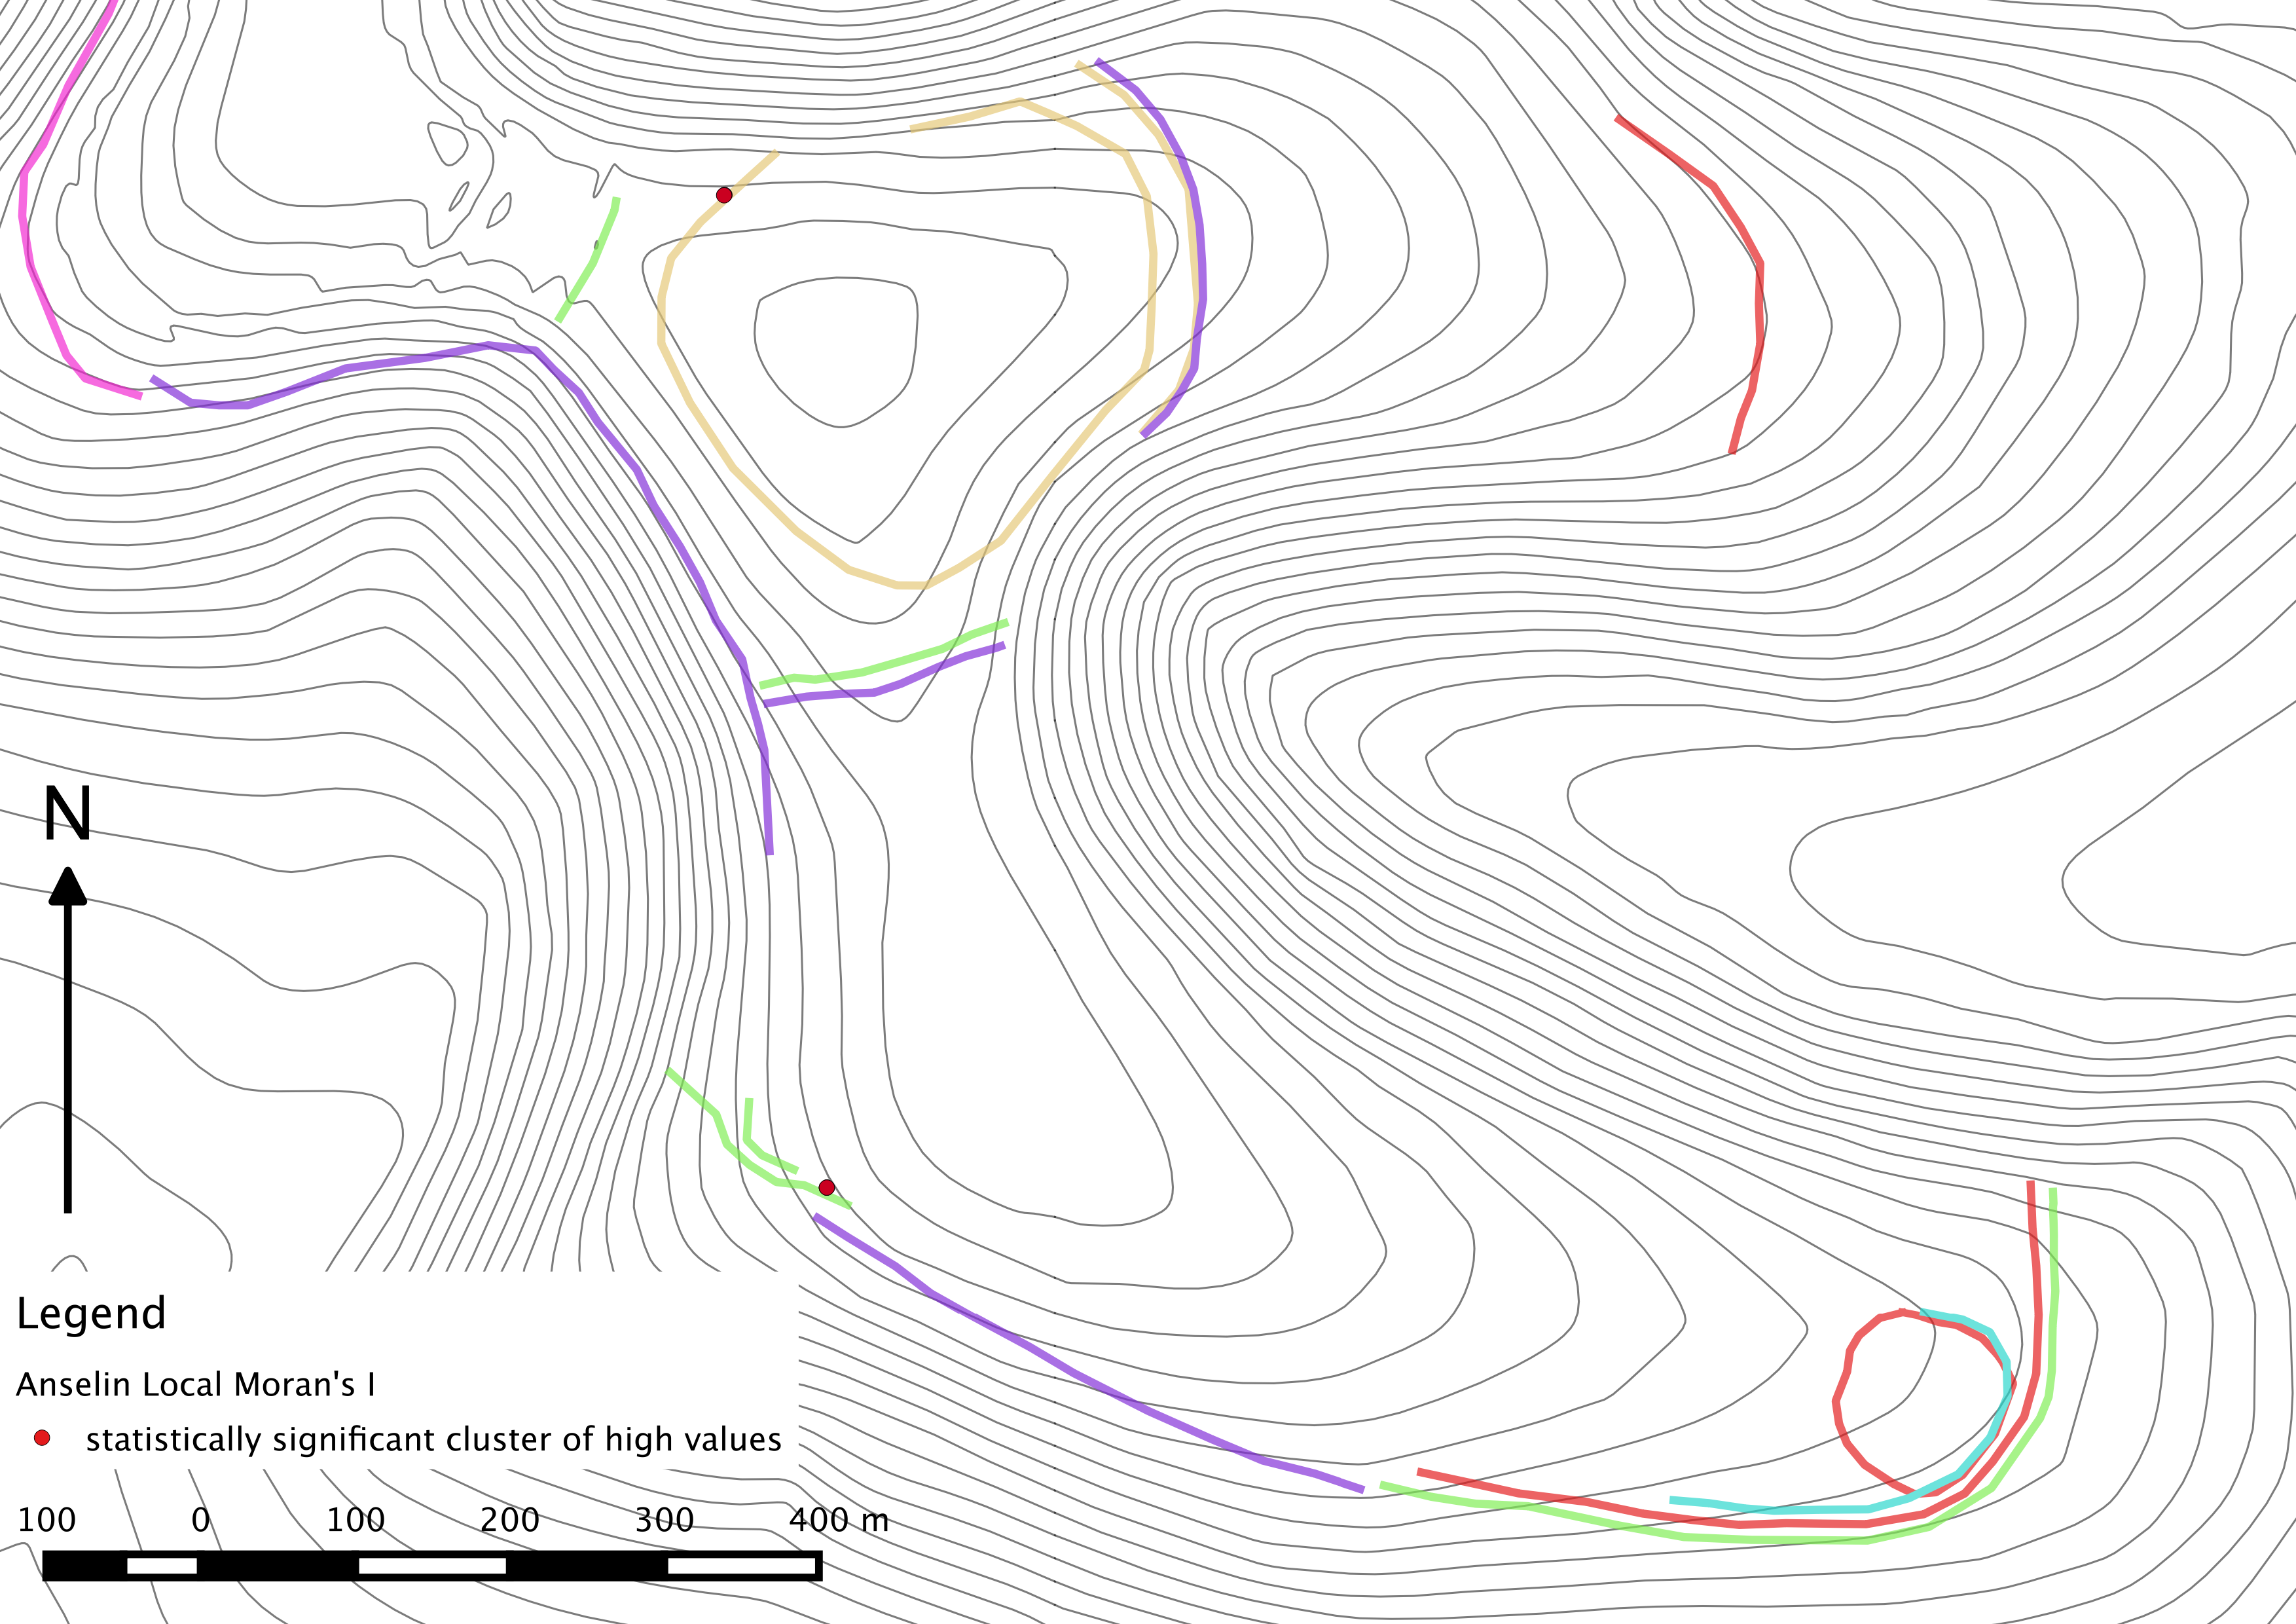
\includegraphics[width=0.8\textwidth]{figures/cluster-HH-mean}
	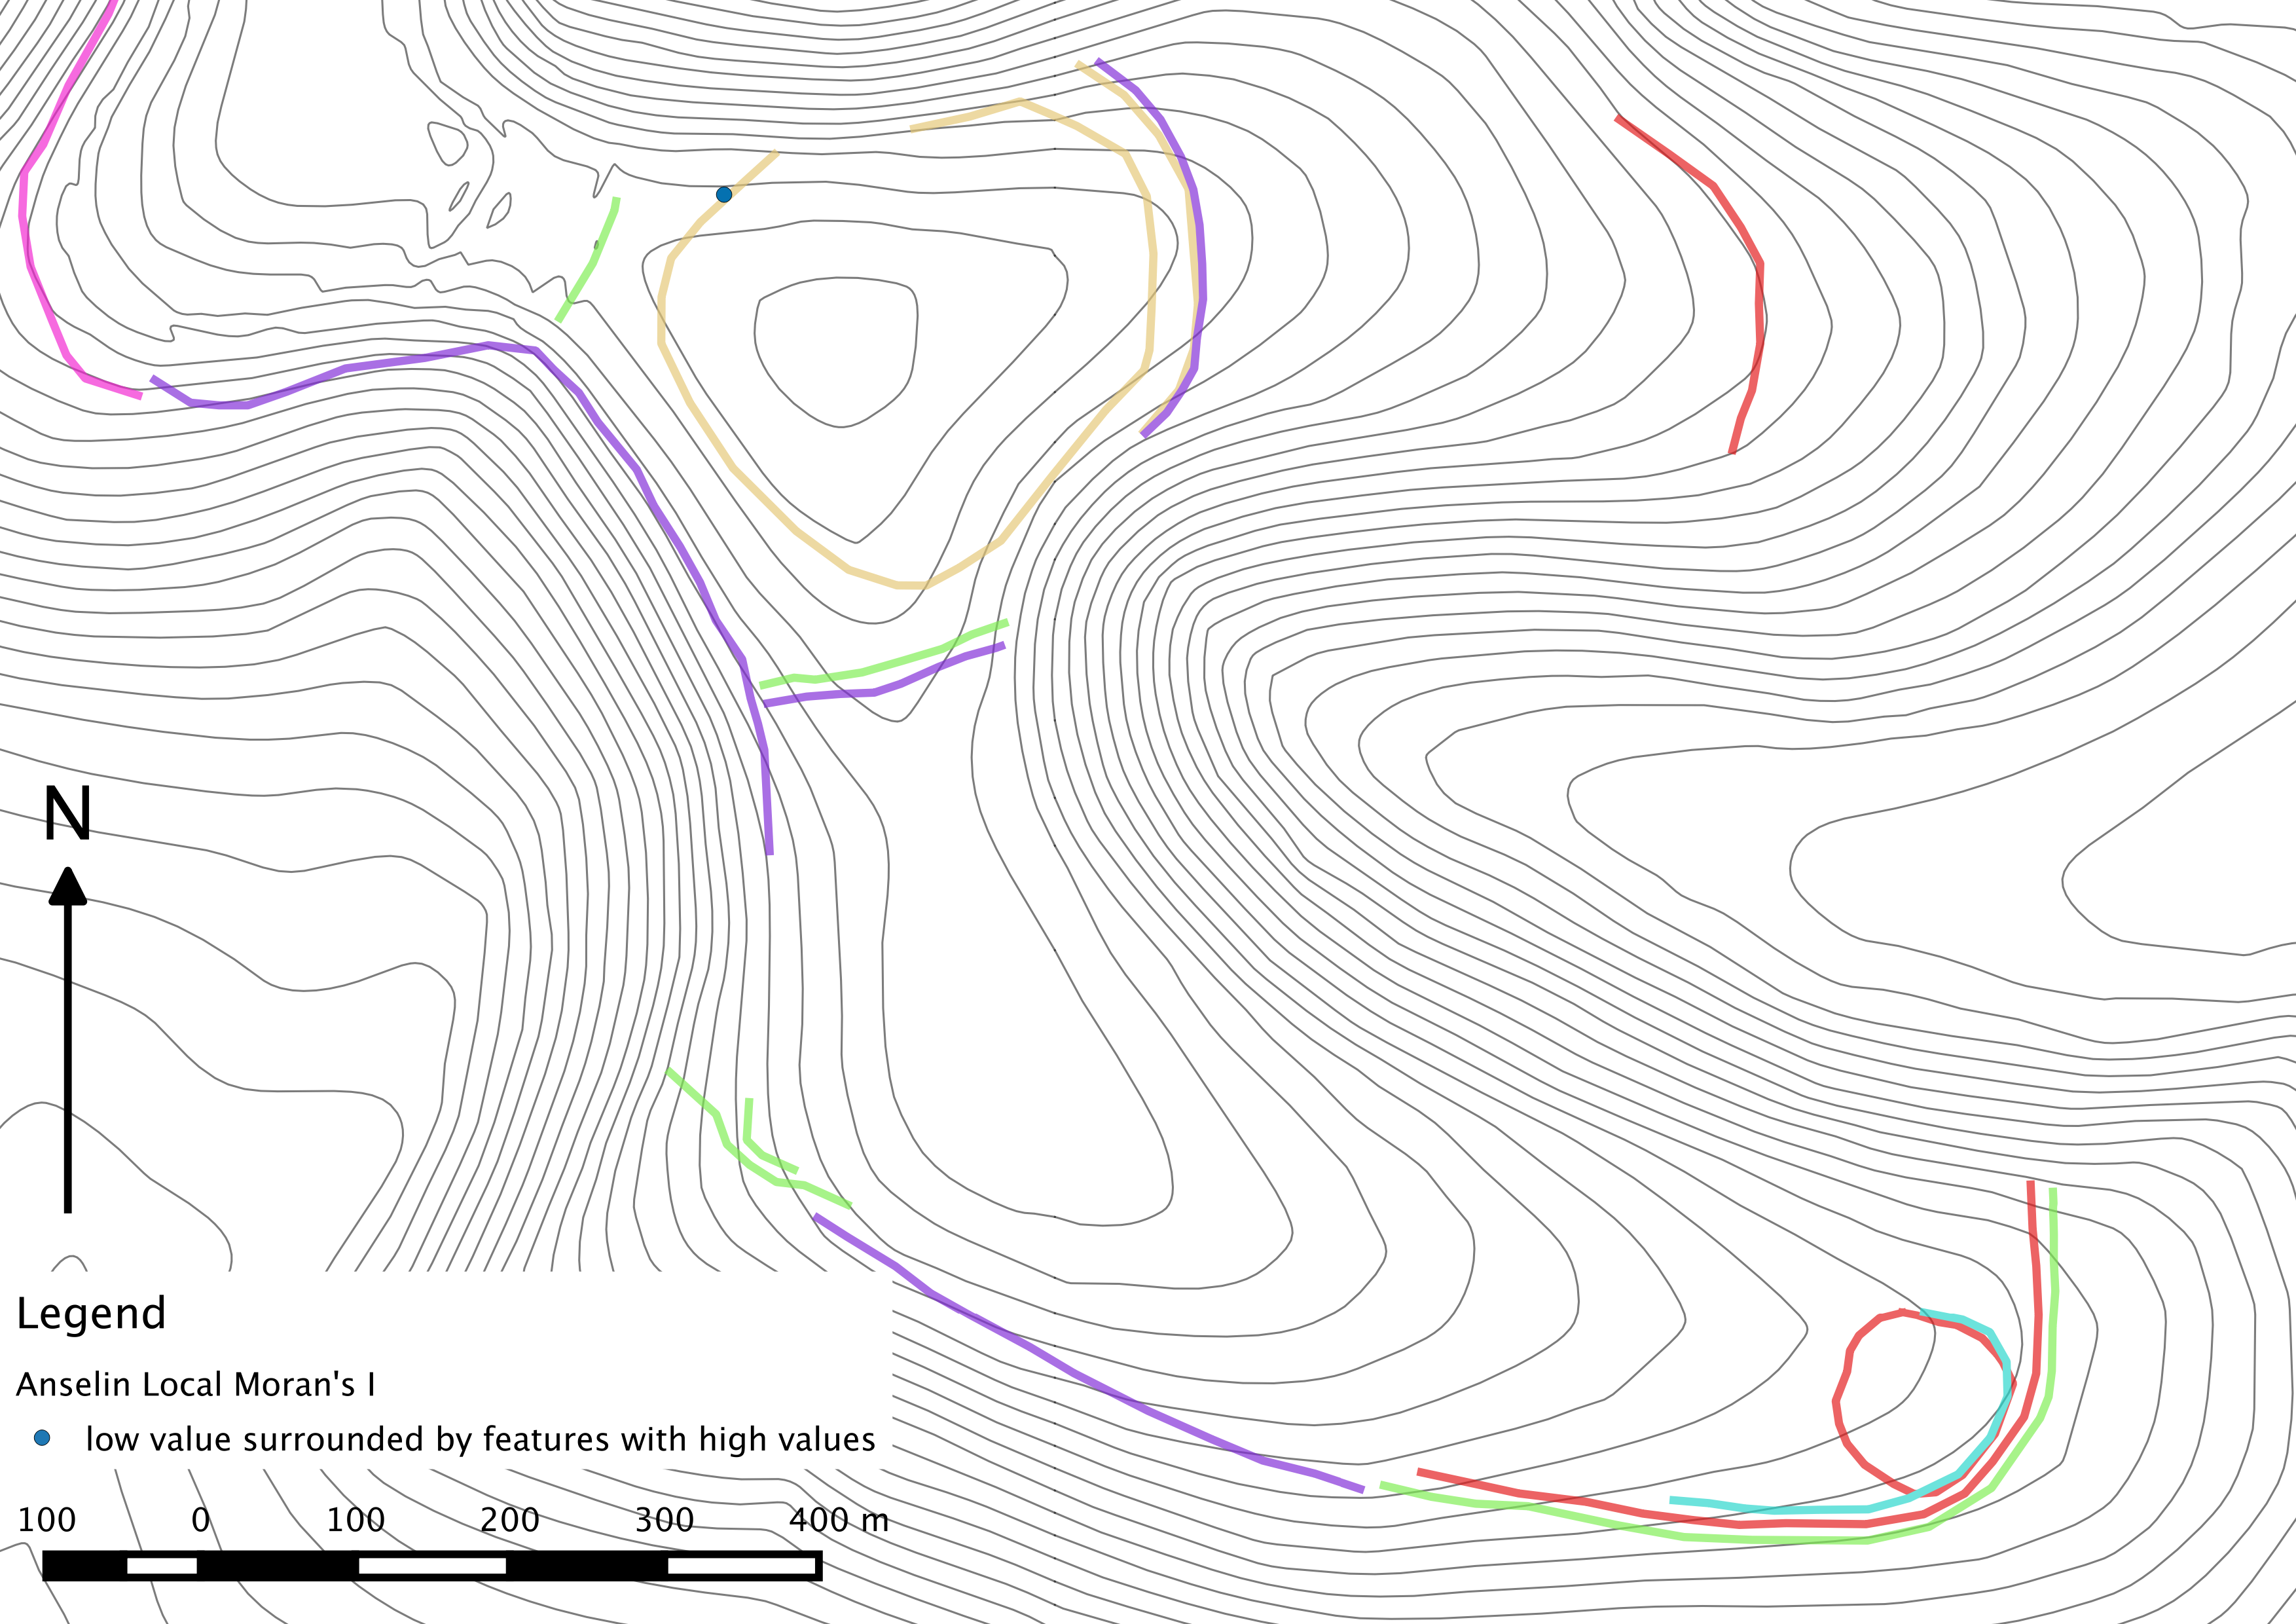
\includegraphics[width=0.8\textwidth]{figures/cluster-LH-mean}
  \caption{Plan of statistically significant clusters and outliers based on a spatial conceptualisation of space}
  \label{fig:cluster-mean}
\end{figure}

As a comparison, figure~\ref{fig:cluster-mean} shows the results of running the Anselin Local Moran's i using the raw spatial locations and their distance as the conceptualisation of space and the mean as the value. This shows the key locations are the same, and analysing the raw results shows that it is in fact the same dates which are identified as clusters and outliers. This suggest the inclusion of chronology and transformation of spatial relationship to a binary value has had little to no effect over the final identification of clusters and outliers. And based on the analysis above, it is clear that the identification of clusters and outliers provides mixed results, some due to facets of the samples and others down to the underlying archaeological data. 

\subsubsection{Getis-Ord Gi*}
Another potentially valuable local statistic is Getis-Ord Gi*, a measure of whether high or low values cluster spatially. The output z-scores shows hot spots and cold spots as large positive and negative z-scores, in this case hot spots are later values surrounded by other later values and cold spots are earlier values surrounded by other earlier values. The values used are the same average value from the posterior density distribution of the bayesian modelled date as used previously.

\begin{figure}
\centering
	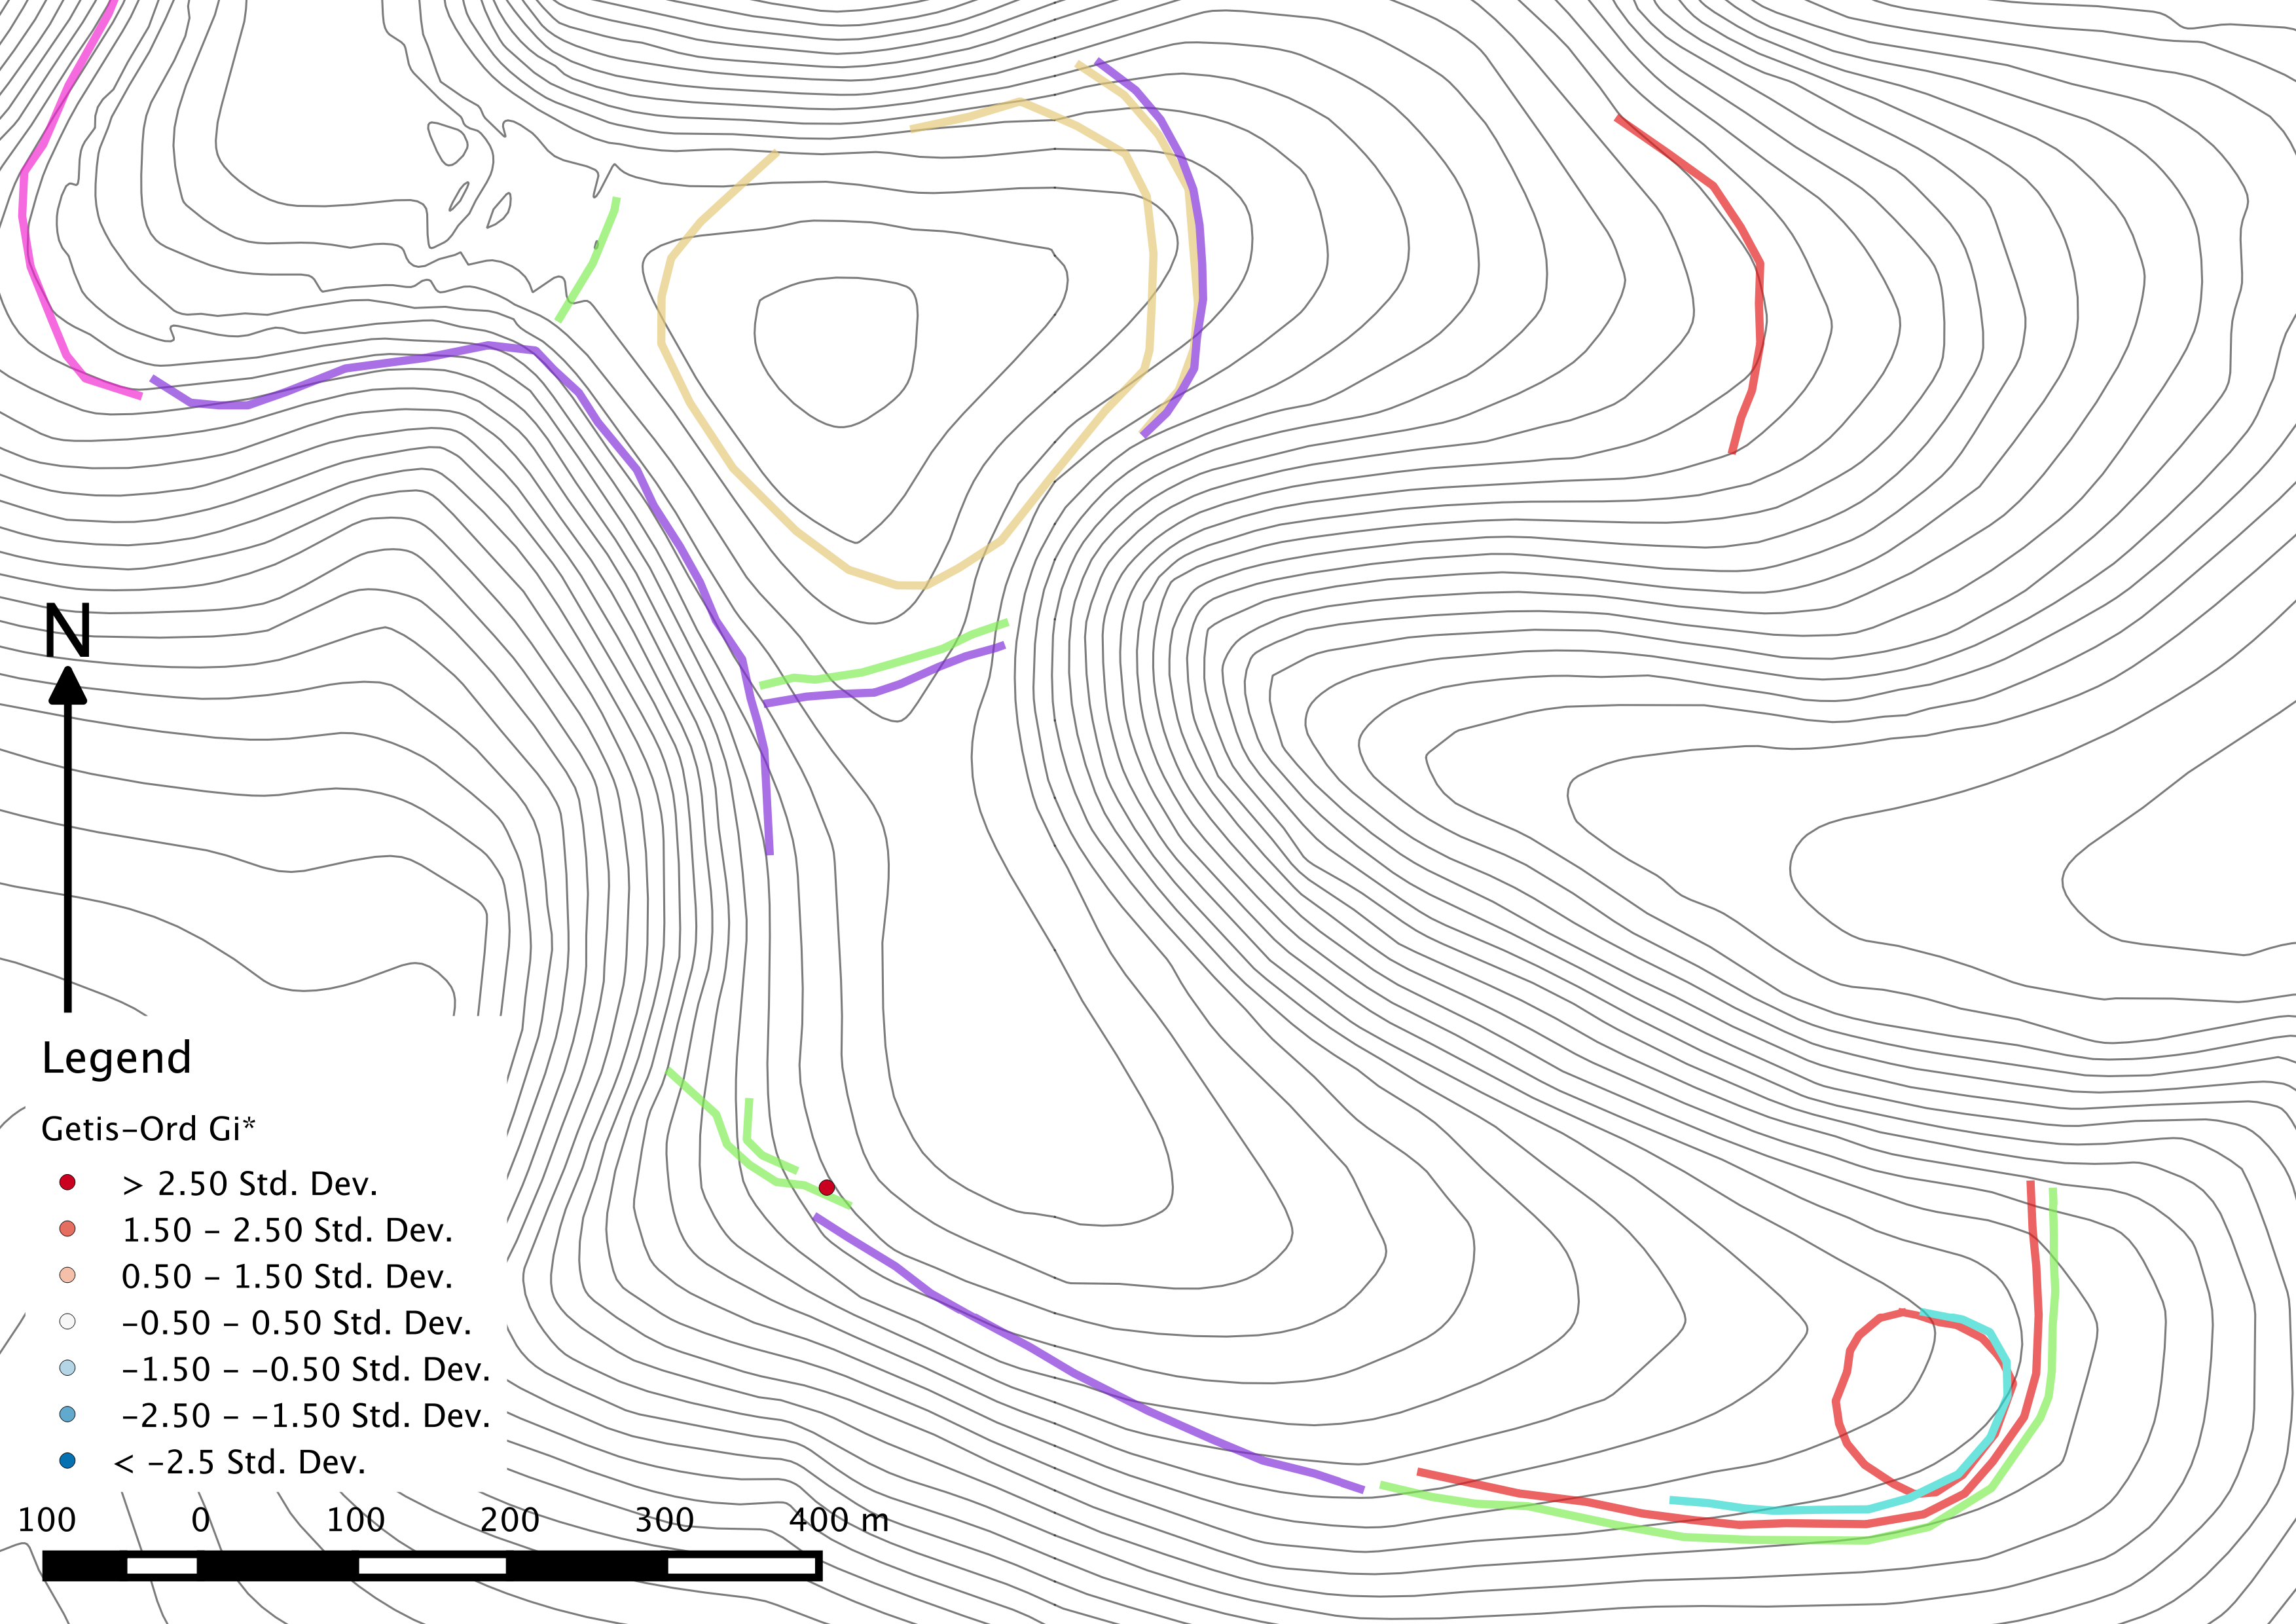
\includegraphics[width=0.8\textwidth]{figures/hotspot-1}
  \caption{Plans of most significant positive z-score values ( $>$ 2.5 Std. Dev.)  for Getis-Ord Gi*}
  \label{fig:hotspot-1}
\end{figure}

\begin{figure}
\centering
	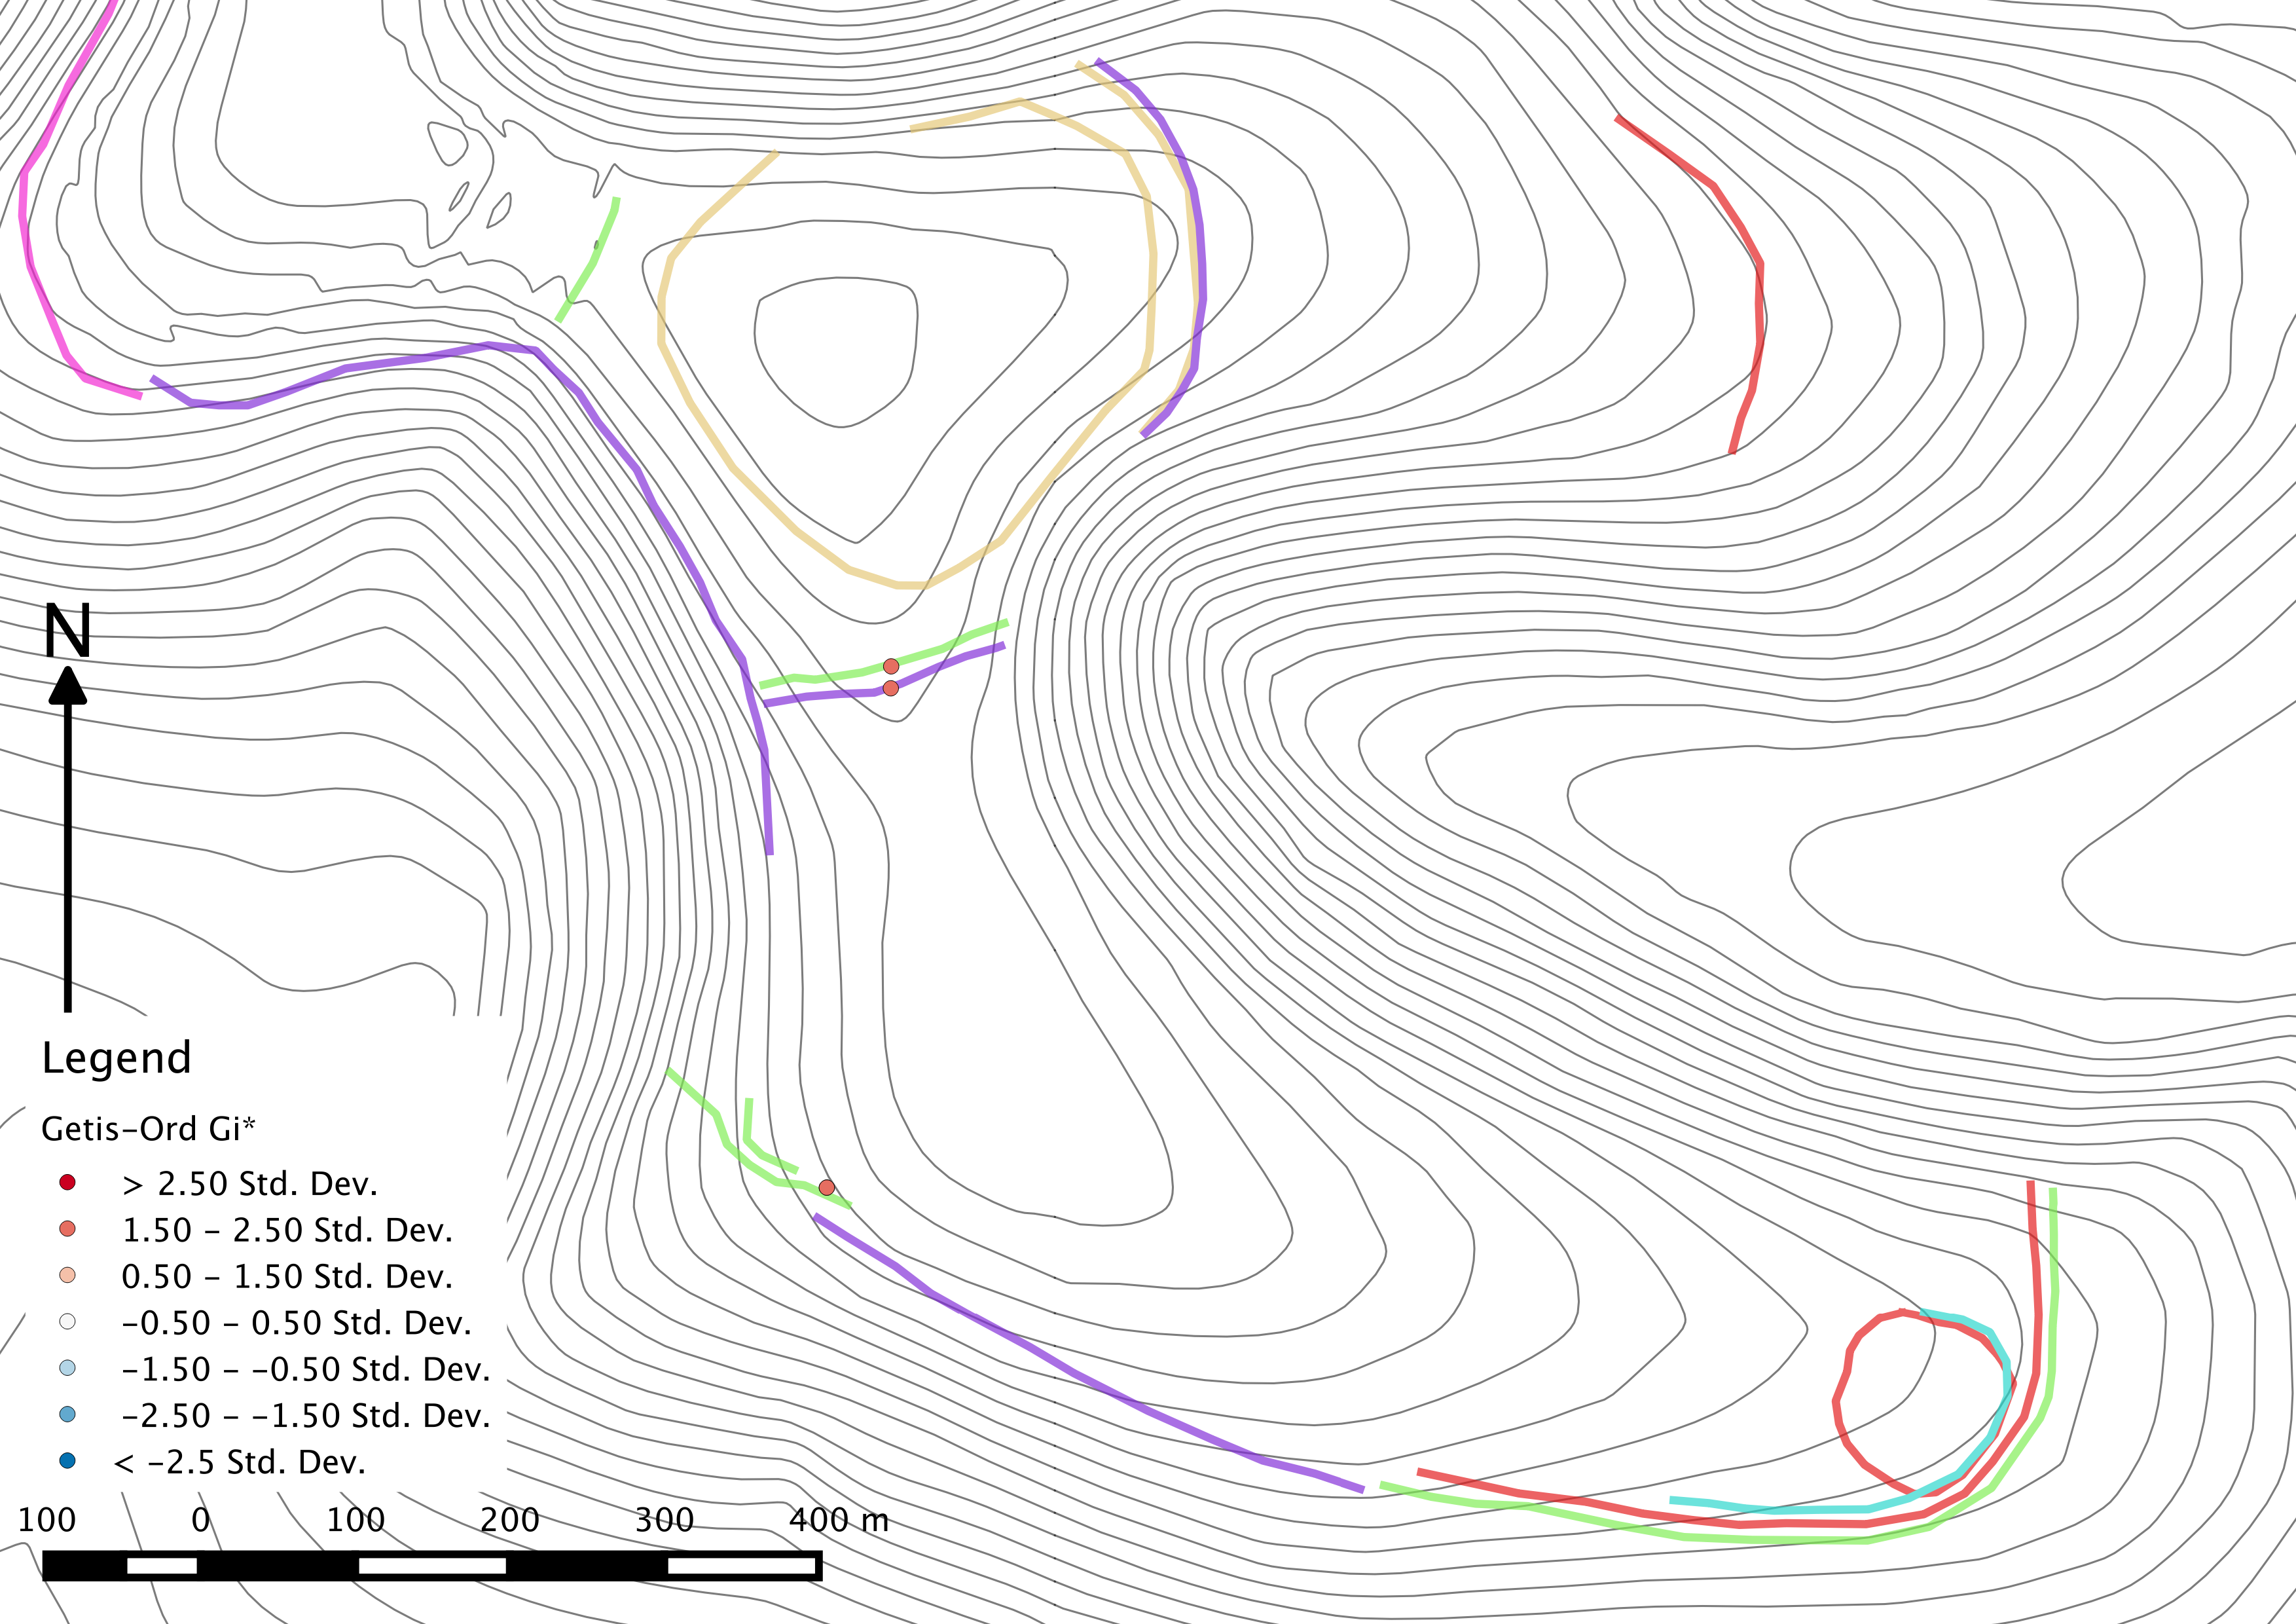
\includegraphics[width=0.8\textwidth]{figures/hotspot-2}
	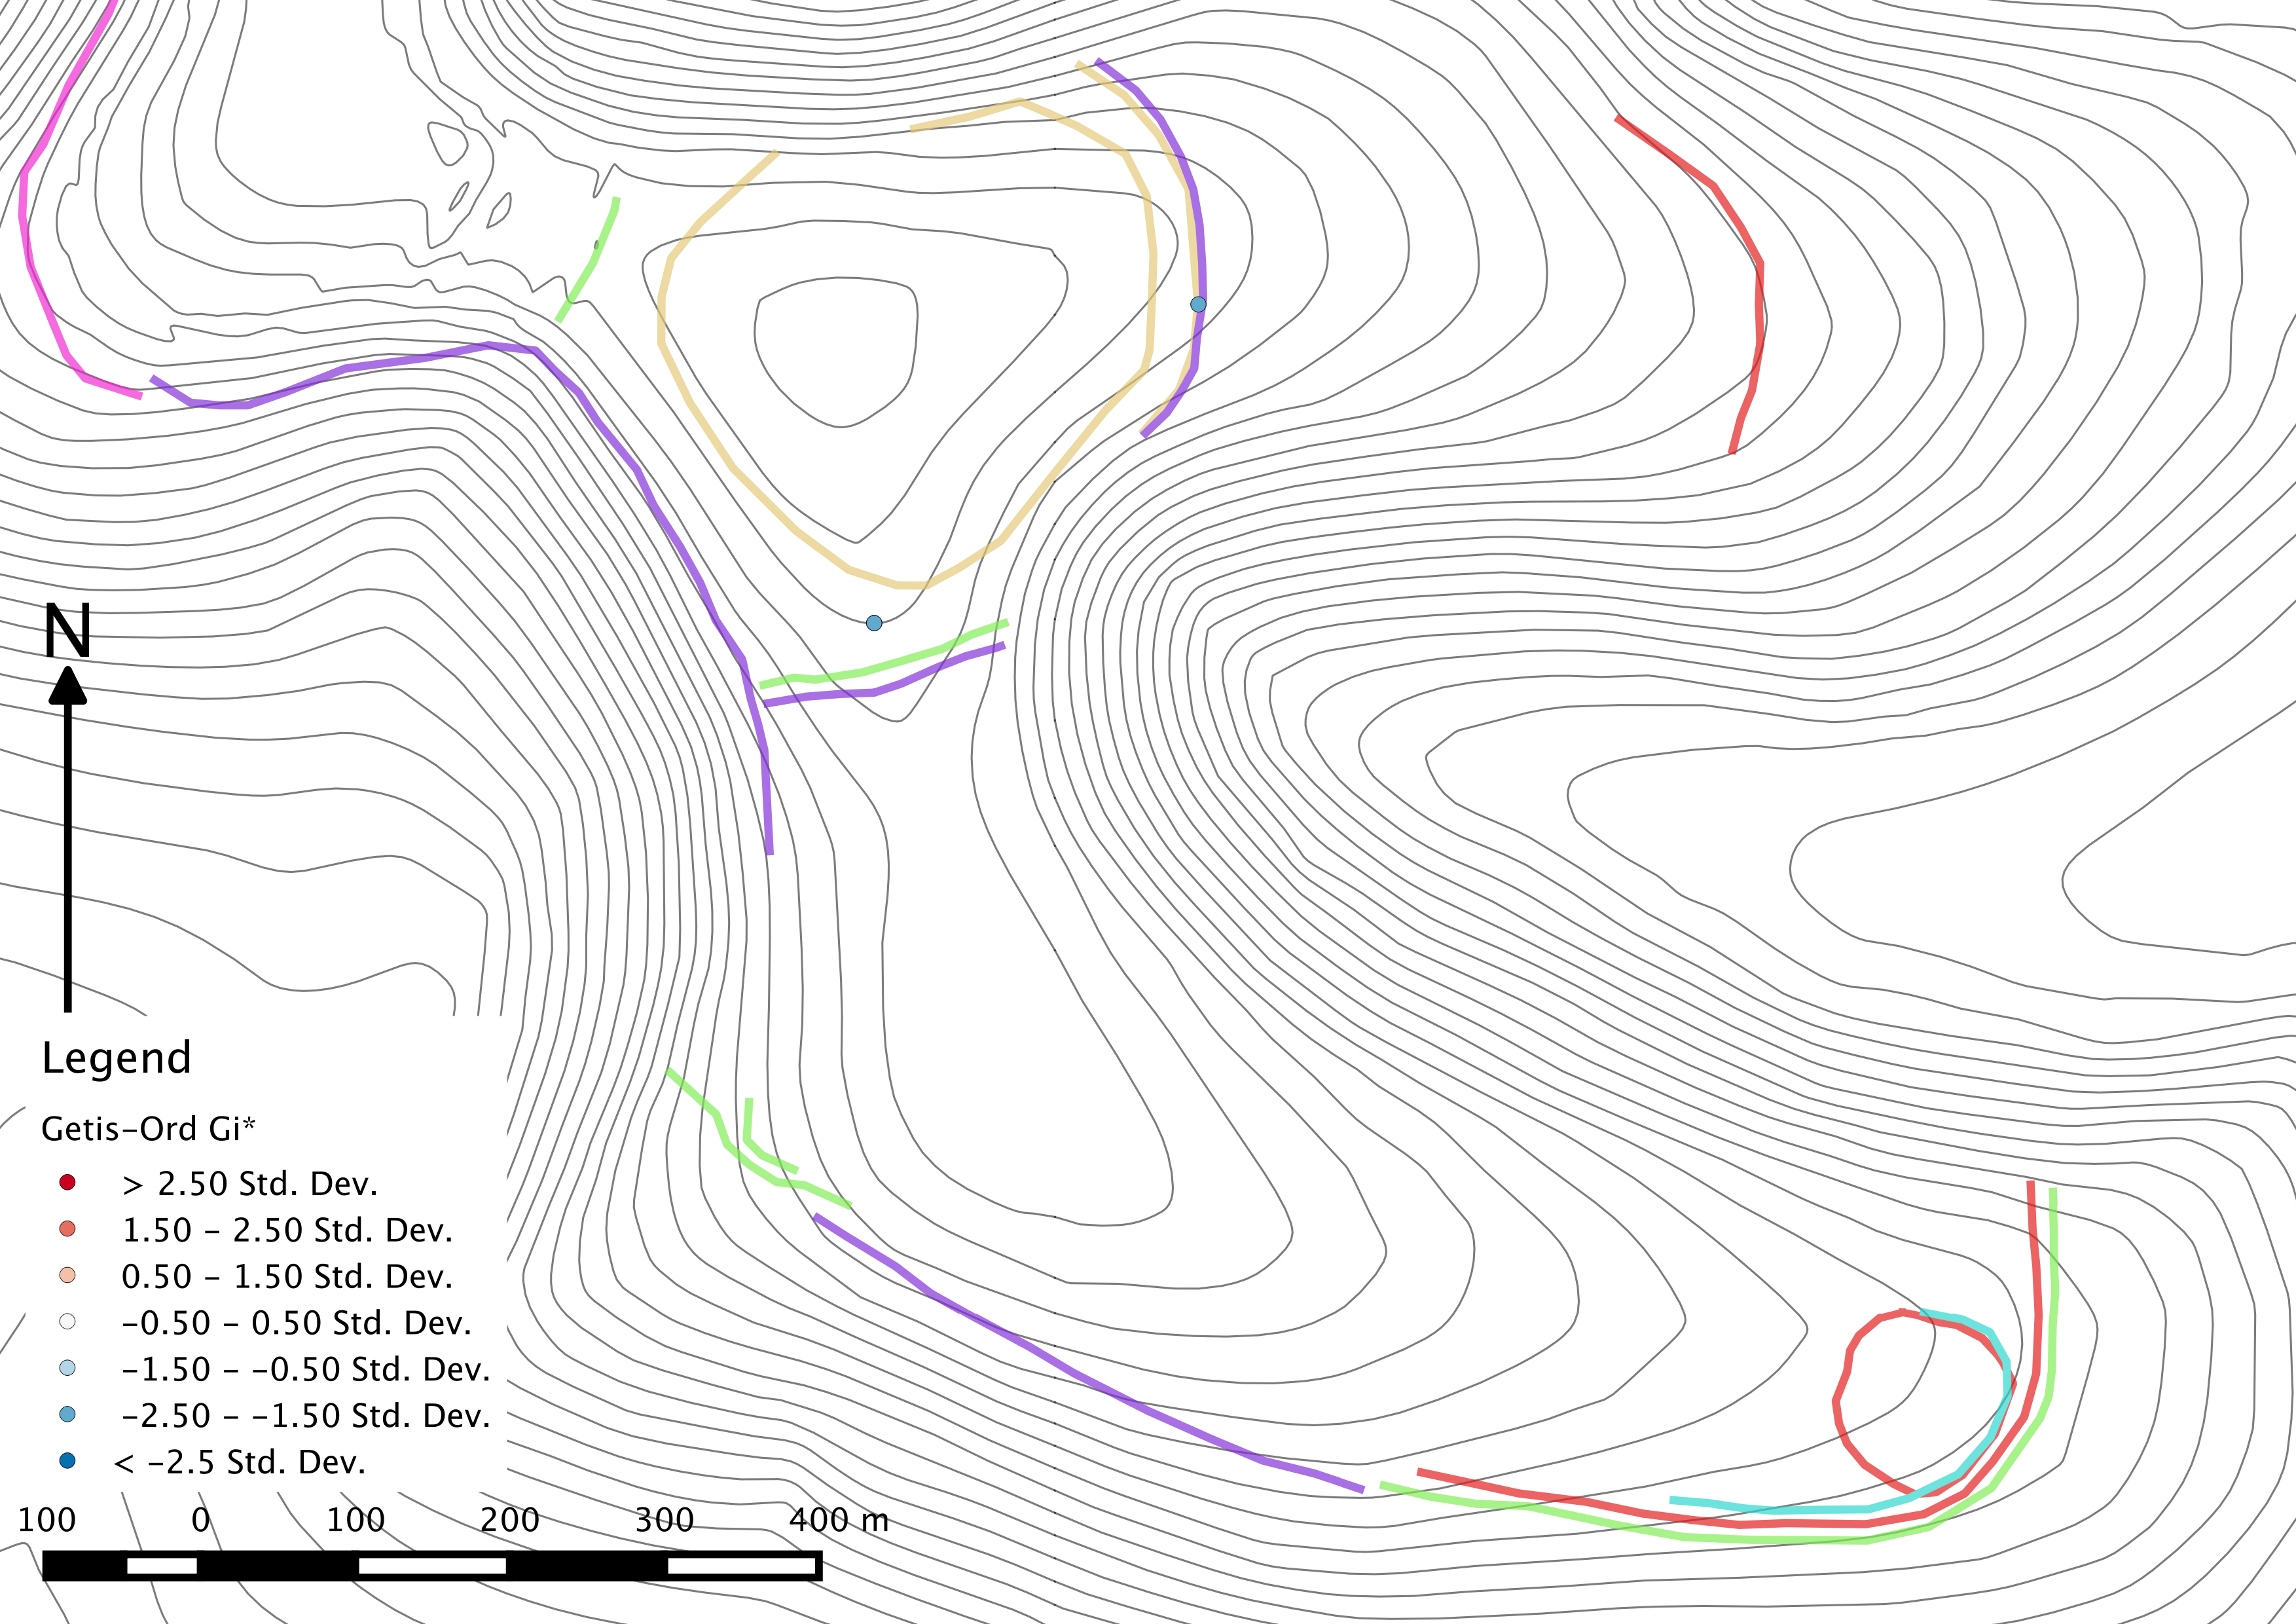
\includegraphics[width=0.8\textwidth]{figures/hotspot-6}
  \caption{Plans of other significant positive and negative z-score values ($>$1.5 and $<$ 2.5 and $<$ -1.5 and $>$ -2.5 Std. Dev.)  for Getis-Ord Gi*}
  \label{fig:hotspot-2}
\end{figure}

\begin{figure}
\centering
	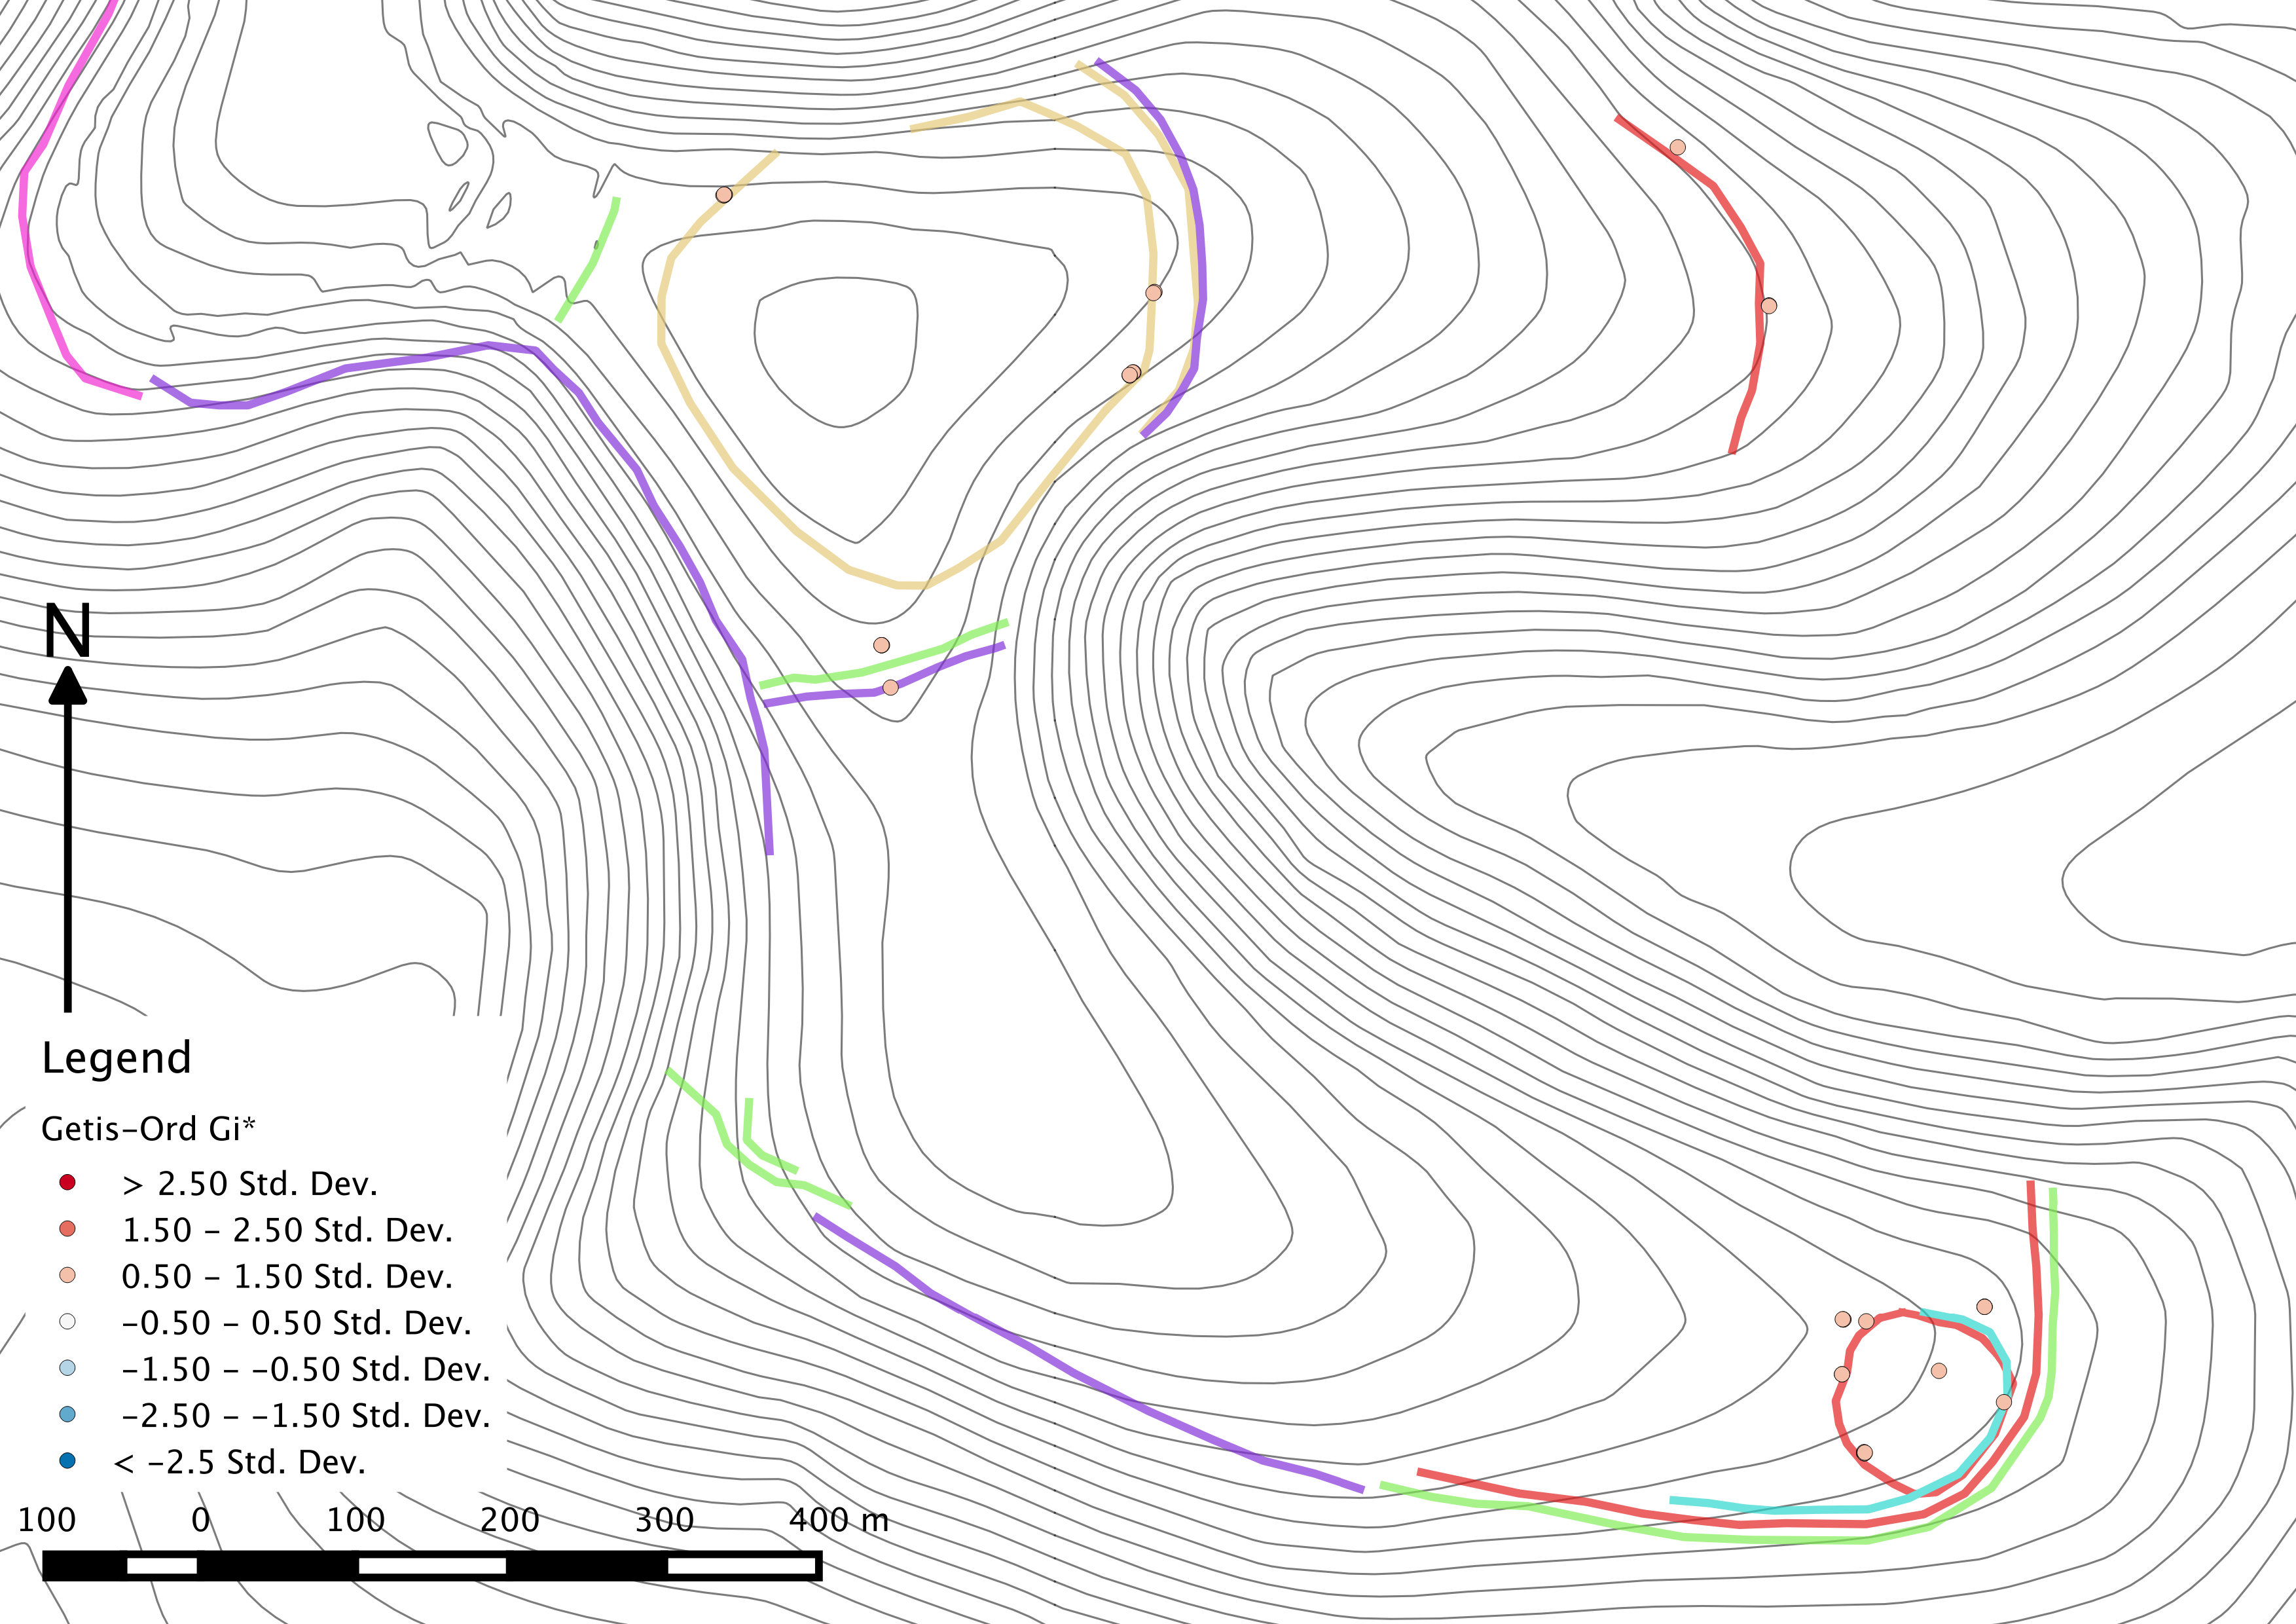
\includegraphics[width=0.7\textwidth]{figures/hotspot-3}
	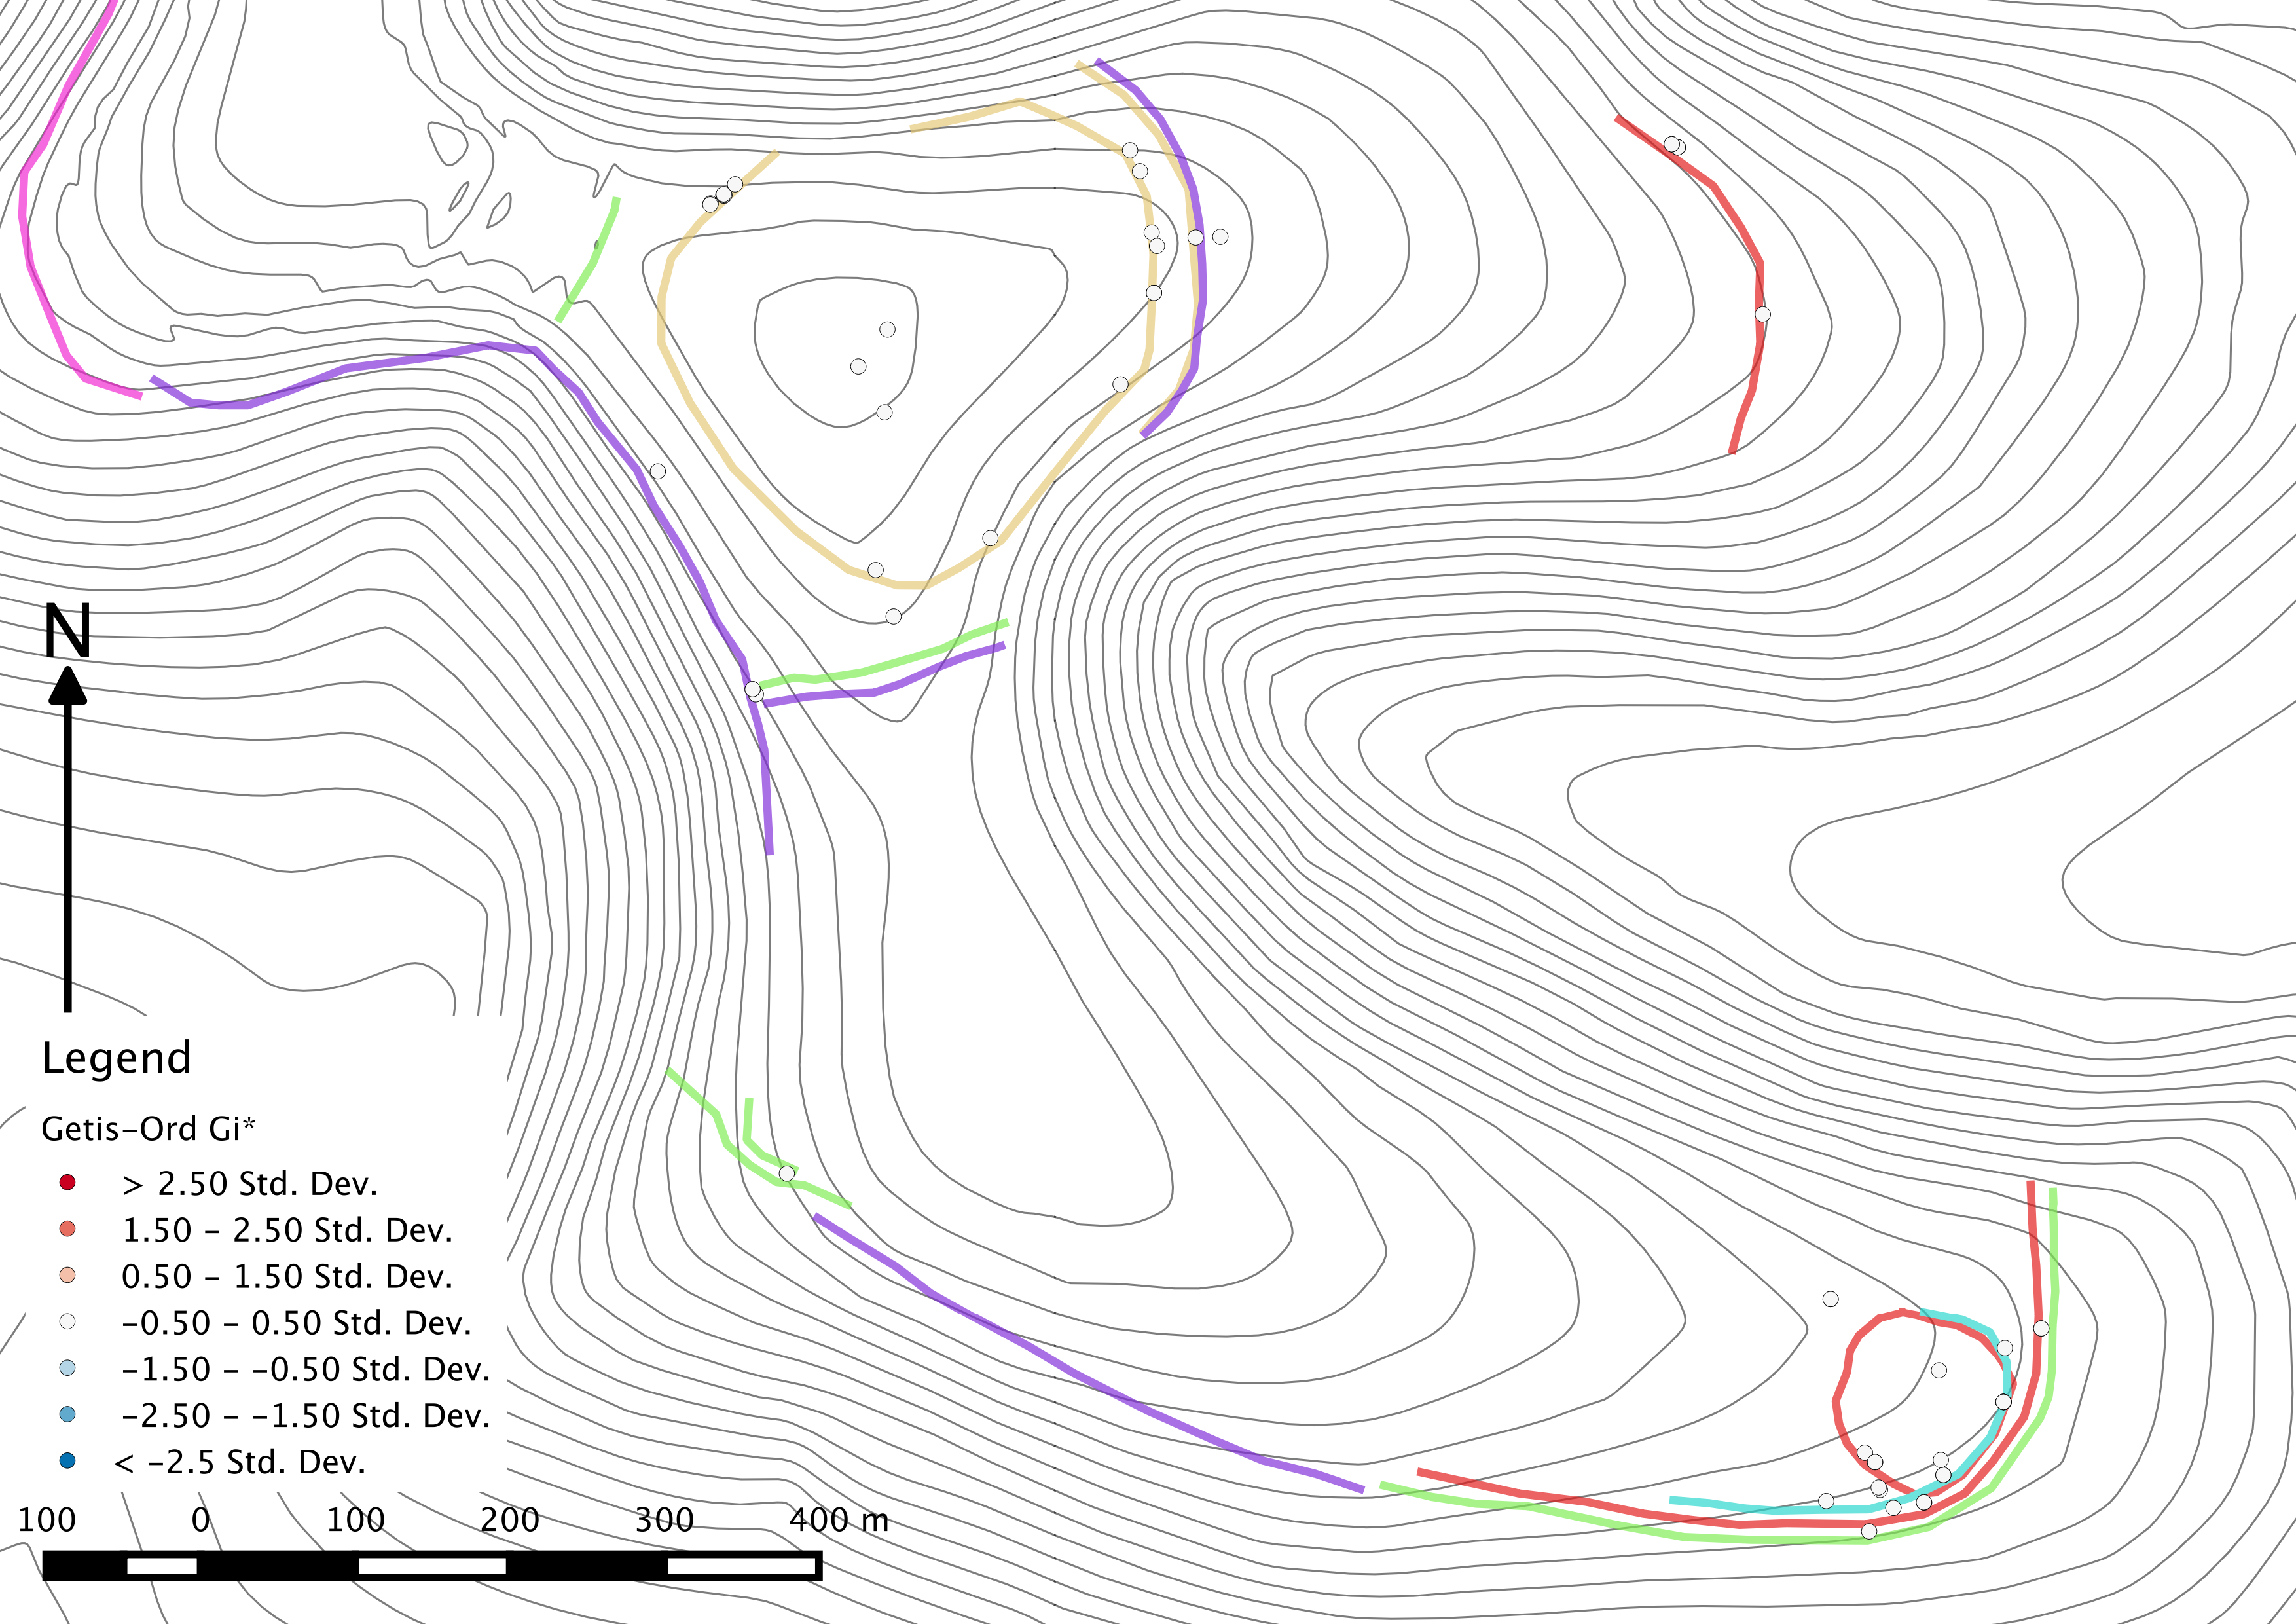
\includegraphics[width=0.7\textwidth]{figures/hotspot-4}
	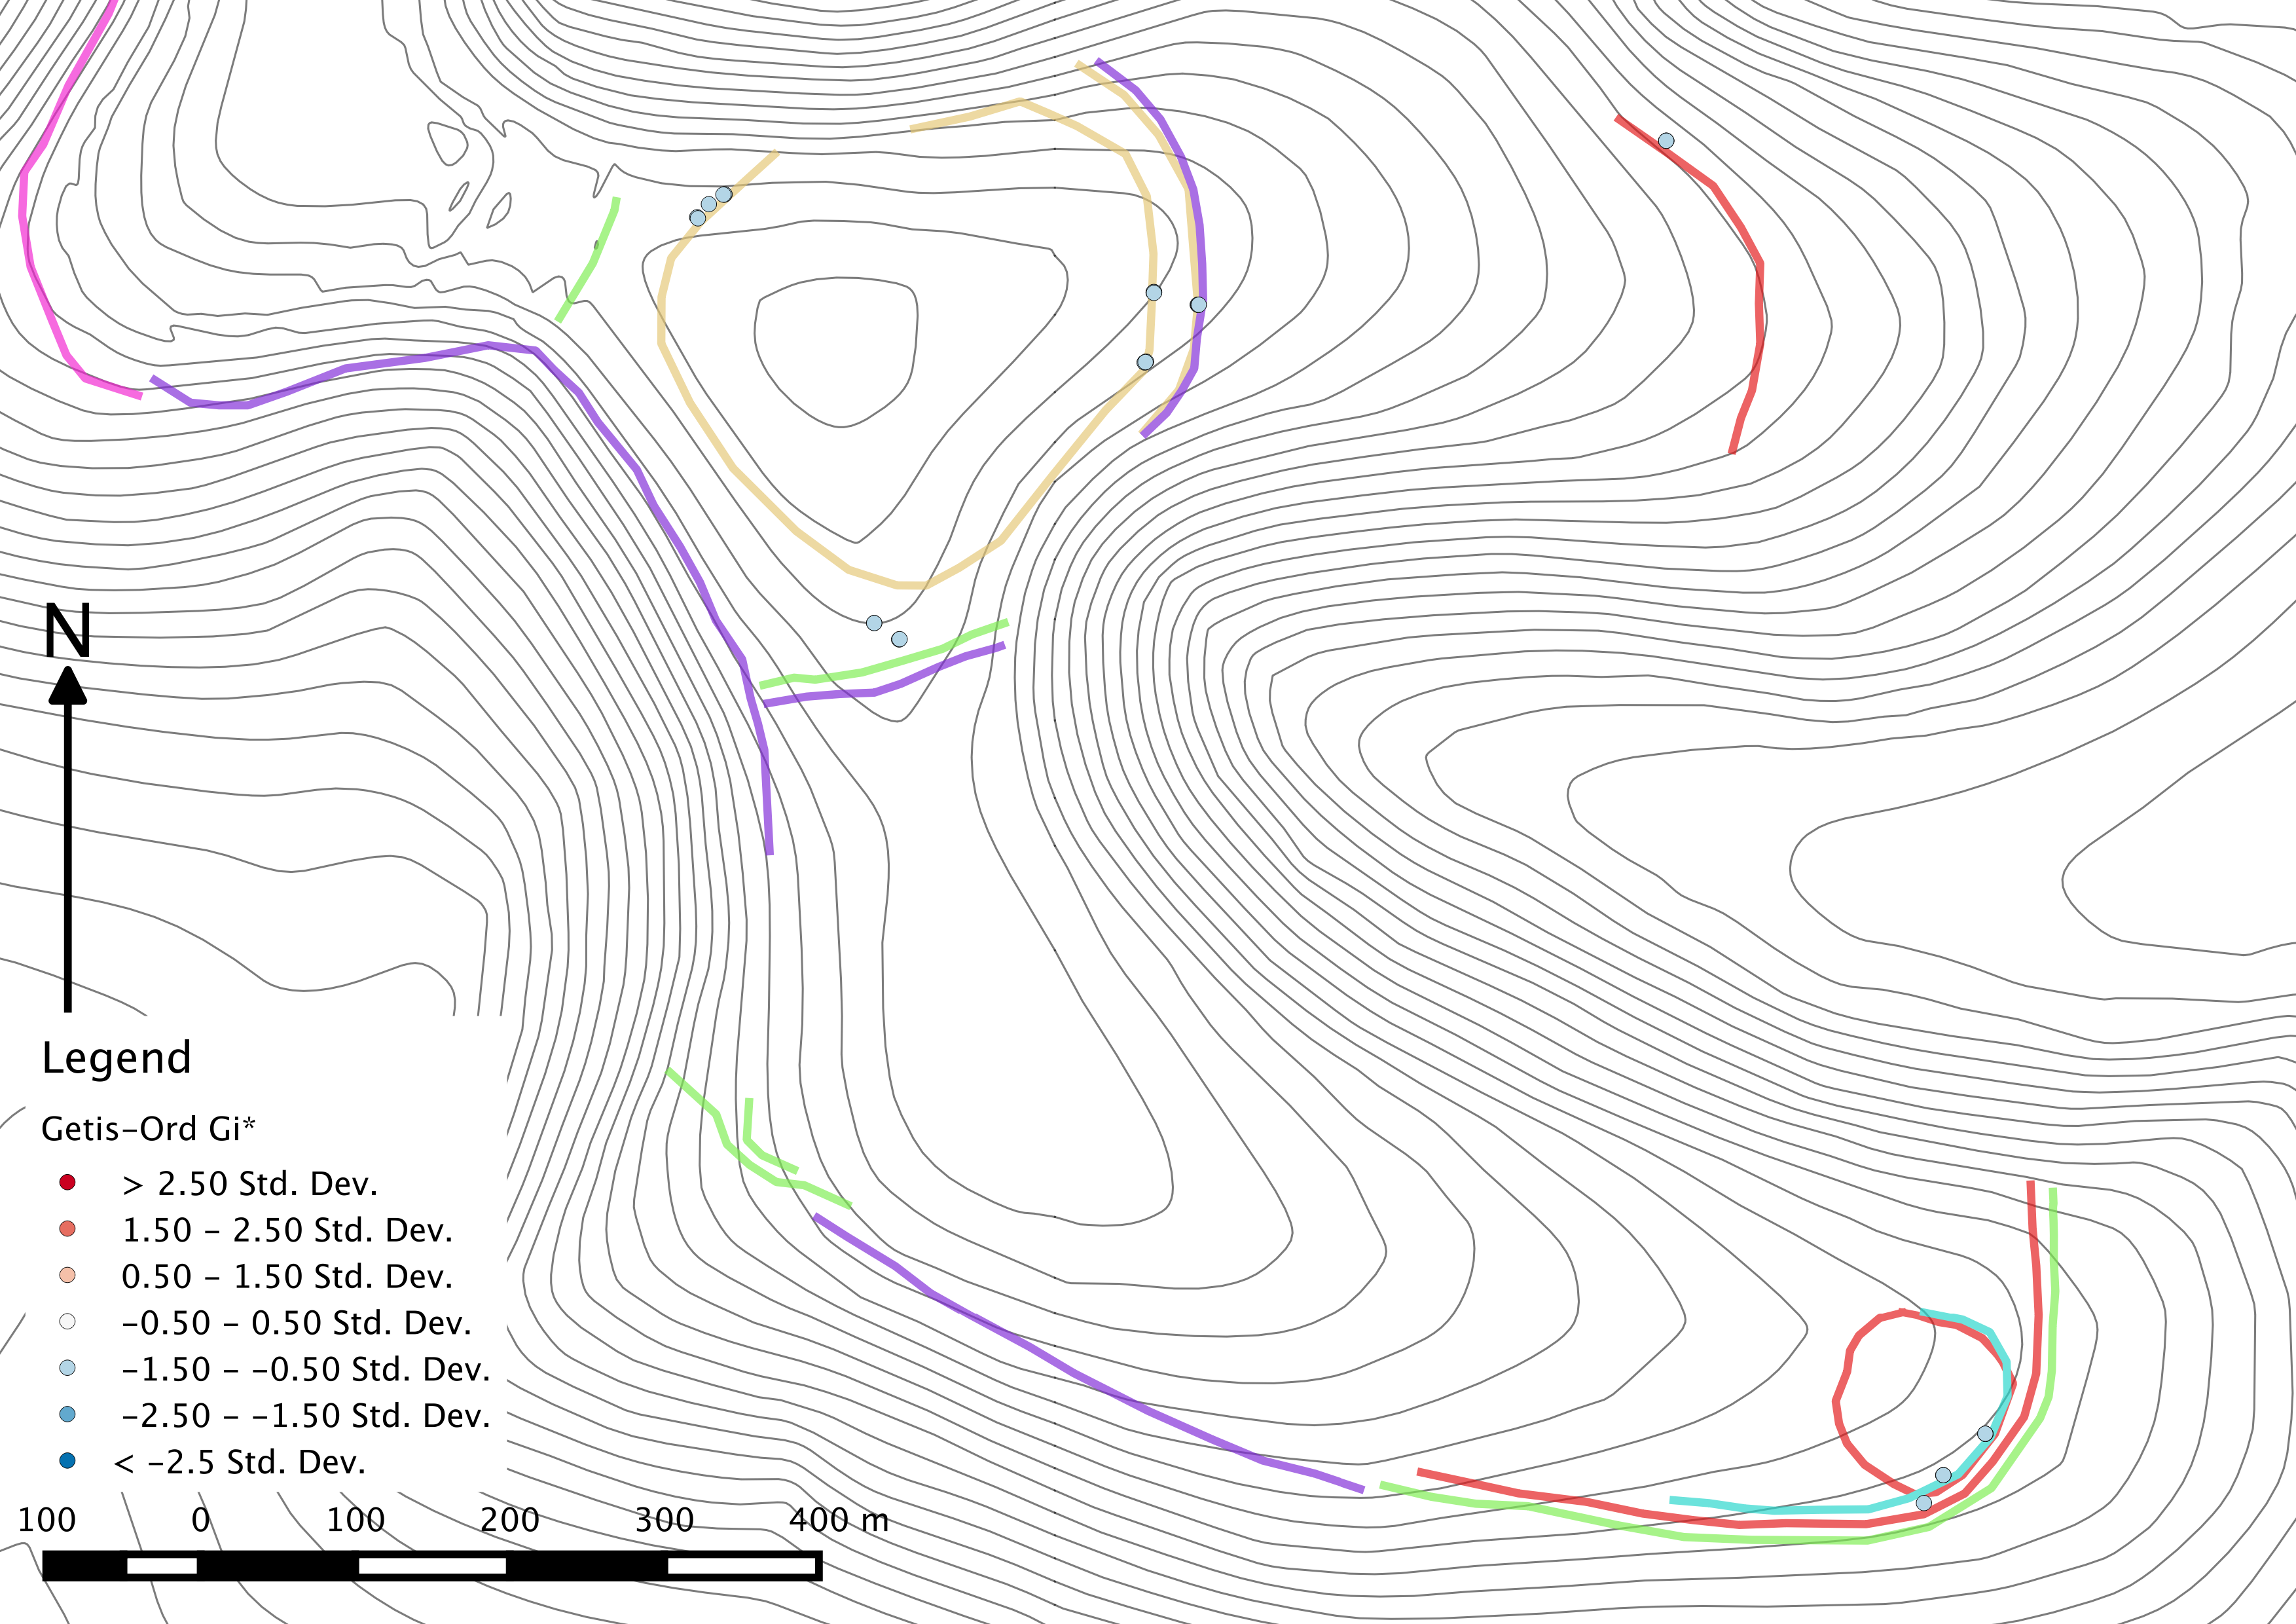
\includegraphics[width=0.7\textwidth]{figures/hotspot-5}
  \caption{Plans of least significant positive and negative z-score values (between +1.5 and -1.5 in steps of one Std. Dev.)  for Getis-Ord Gi*}
  \label{fig:hotspot-3}
\end{figure}

Figure~\ref{fig:hotspot-1} shows the most significant hot spots calculated using Getis-Ord Gi*, (there are no correspondingly significant cold spots). There is only one such value, located in the Hanford Outworks, HAR-6038. This was taken from bulked unidentified charcoal, and is modelled as in phase with two other dates UB-4271 and UB-4272 at the same location, there is also date OxA-7850 from the Hanford Outworks. In interpreting this hot spot, it is important to remember that the date values used were averages from the probability distribution (-3424 B.C., -3326  B.C., -3329  B.C. and -3546  B.C.). In this case the distributions of the three dates in phase were very similar, which will have resulted in average values that were also very close together. As there are only four dates from this part of the site included in the bayesian model, a hot spot here indicates this is an area which would benefit from having more samples dated.

Figure~\ref{fig:hotspot-2} shows significant positive, and significant cold spots. There are four such positive hot spots. From the inner south cross dyke is UB-4268 and OxA-7825. This feature also provided sample OxA-7826, respectively they have mean dates of -3553  B.C., -3410  B.C. and -3350  B.C. In this part of the site, there is also the southern long barrow (nine dates, averages from -3638 to -3403), western outworks (OxA-8861, -3576 B.C. and OxA-8862 -3542 B.C.) and segments from the central enclosure (OxA-8851, -3627 B.C.). This hot spot is potentially an identifiable focus of activity, although the particular dates must be treated with the utmost caution as they are averages from the probability distribution. The different features are identified as coming from distinct phases in the chronology, with the main enclosure and long barrow coming from period 1A, the inner south cross dyke from period three and the western outwork from period four. The bayesian model for the inner south cross dyke has two components. From the pre-inner south cross-dyke there are two dates, (OxA-8861 and OxA-8862) which are in fact from the western outwork (and are of Boreal date), but included in this part of the model due to its stratigraphy. And from the recuts phase, date UB-4273 is also actually from the western outwork. This ultimately leaves very few dates from the rest of the inner south cross-dyke, (OxA-7825, OxA-7826, NPL-76, UB-4268) with two coming from the same context (OxA-7825 and OxA-7826) so the close averages for these dates must be a strong factor in its identification as a hotspot. 

UB-4272 and UB-4271 are from the Hanford Outworks, and are related to the hot spot from figure~\ref{fig:hotspot-1}.

Figure~\ref{fig:hotspot-2} also shows three significant cold spots. Two are from the south long barrow (OxA-8847 and OxA-8848 with mean dates of -3596 and -3571). There are ten dates from the south long barrow and an inspection of the model, reproduced in figure~\ref{fig:crossdykes} clearly shows that this particular cold spot is not simply a facet of the averages, but the closeness of the modelled dates is visually apparent as well. These two dates are both from LB2 (the barrow being excavated in quarters) and from phase one in the stratigraphic model, along with OxA-8846 and OxA-7848, which also show the same homogeneity in the underlying probability distribution. Other dates in the model, which are close in space and time, also share a very similar probability distribution, this would combine to create the strong cold spot identified by the algorithm. However, it is crucial to note that four of these dates are in fact from the same layer of primary silt, OxA-7848, OxA-8846, OxaA-8847 and OxA-8848. This may ultimately mean that this particular area has had a disproportionate affect on the algorithm, and draws our attention to an important theme on the nature of archaeological data. This is to what extent can archaeological data be treated as a random sample (for the purposes of performing statistical analysis)? In this case, that data points are not spread randomly through space and time, there being a cluster of such points in the same long barrow ditch, from the same phase. It is perhaps not surprising that such a cluster would be identified as a hot (or cold) spot.

The other is from the inner east cross dyke (OxA-8856 with mean date of -3547). There were a total of six dates from this feature, (OxA-8893 was accidentally omitted from the model, Alex Bayliss, personal communication) of which, OxA-8856 and OxA-8857 belong to the same context in segment four, three belong to another context in segment four and the other is from segment five. The model, figure~\ref{fig:crossdykes}, shows high agreement among the dates, apart from OxA-8857. As before, this cold spot may be an identified locus of activity, or it may be an artefact of the available data. In this case the latter seems likely due to the very limited spatial and temporal spread and the small number of dates in this area.

While both of these cold spots have limited dates in the immediate locality, there are a greater numbers of dates in the wider area and across neighbouring features, which suggests that while the data has clearly had an effect, it may not be quite so clear cut, the cold spots could also be an indicator of an area that was a focus of activity. 

Figure~\ref{fig:hotspot-3} show the remaining date values, with the z-score values split into three groups. These figures includes all other values, so they are not regarded as significant, or worth further investigation based on the z-score alone.

\subsection{The Value of Quantitative Approaches}
These results are not providing earth shattering insights into the lives of past people, but they are descriptive of the data, the same data that has been used to draw insights into the archaeology of Hambledon Hill. The benefits of using such techniques is a more thorough understanding of the data available, which can be used to ensure that any conclusions drawn from that data respect its limitations. 

At Hambledon, the global Moran's i has provided a numeric basis for an observation on the data, that dates within features show positive autocorrelation. Across the site, within features, dates will tend to be chronologically close, rather than evenly spread out. The weighting used here is based on only a 1-dimensional representation of space, which could be improved upon. If the dates were recorded with a more detailed location, this would make that easier - although it would still be necessary to calculate a single weight value from both the spatial distance and the temporal. Without this data it is either a case of calculating a less detailed metric, as above, or creating a false sense of accuracy by assigning co-ordinates to each date. Crucially the global metric is a relatively cheap way of confirming an observation, and informing a route for a more detailed investigation, using local measures.

The Anselin Local Moran's i draws our attention to two areas of the site, one offers a detailed view of a segment of the site's chronology, showing the potential for a detailed interpretation of areas that have a spread of dates through the chronology. And the other, a location where multiple dates on the same samples or contexts made up a large part of the chronology, which could benefit from more dates, spread through the chronology. Clearly the results of this method require detailed investigation as they offer very different opportunities, despite both being represented as clusters around certain date values. The technique enables us to probe parts of the site at both ends of the spectrum in terms of the detail provided by their chronology, while it can offer interpretative opportunities, the technique itself is primarily descriptive of the data set.

The Getis-Ord Gi* analysis was able to identify a number of clusters, several regarded as significant hot or cold spots. In this case, all the areas identified are probably due to there only being a small number of dates in the particular area, that have come from relatively close parts of the chronology and so have close enough average values to be identified as a hot (or cold) spot.
The Hanford outworks, which was also identified by the Local Moran's i, is identified twice by the Getis-Ord Gi* analysis, it is clearly an area of the site that would benefit considerably from more investigation, ideally leading to more dates distributed through its chronology. The re-analysis of section 17, above, demonstrates the added value of this, where a single date (or where only a single context or phase is dated) simply provides a point in time, where as successive dates enable a discussion around duration, a consideration of the passage of time, how the site changed and was modified and across what length of time. Crucially, a series of dates enables the bayesian statistical method to work most effectively and remove some uncertainty (with certain modelled assumptions) from the date values.

Also identified by the Getis-Ord Gi* analysis is a hot spot at the inner south cross dyke, however a detailed analysis of the data reveals that, again this is an area with very few dates, with limited spread through the chronology. As with the Hanford outwork, what has been identified here is an area of limited temporal evidence, where any detailed interpretation should be treated with the utmost caution. In addition to this there are two distinct areas of cold spots, one at the south long barrow, and the other at the inner east cross dyke. The south long barrow could potentially be either a cluster of activity, or a facet of the data, there are a large number of dates, which span the chronology of the feature (ten dates across five phases) however, half of the dates come from a single phase, phase I and in fact four are from the primary fill. The other dates, (of which two are from the same sample) come from later phases and are dated to much later, potentially in the region of 150 years later or so. This would in fact suggest that the cold spot in this case is down to the dates in the model not being evenly spread through the chronology, but concentrated (or clustered) in the very first part of the feature's life, the primary fills. This demonstrates that while the number of dates is clearly important, it is much more valuable to have the dates spread through the chronology.

The other cold spot, the inner east cross dyke, has as much spatial breadth as temporal in the available data. Three separate contexts were dated, across two segments, and the two dates from segment four both came from the same layer in the primary sit. As does the date from segment five. Chronologically this is in many regards one dimensional, as there is little scope for detailed interpretation when the dates all come from the same part of the features life, even if there are multiple dates spread spatially. It does permit a limited comparison of the two segments, but this would have to be treated with caution, as there is so little dating evidence available.

The methods evaluated above demonstrate the value of performing combined spatio-temporal analysis. Mathematically they can be performed relatively cheaply if a single value proxy to the true probability distribution of the radiocarbon dates is used, but this must be kept in mind when examining results. While there are mathematical ways of performing cluster analysis on probability distributions, with which it might be possible to perform these analysis on the raw data, it is unlikely that the results will be more valuable, and depending on the precise method of cluster analysis, might in fact make interpretation more difficult. The identification of spatio-temporal autocorrelation is an important characteristic of the data set, and it must be kept in mind that this could potentially be the result of a range of different processes. It is possible that any auto-correlation is a result of how the archaeological deposits were laid down, and offers evidence directly pertinent to the interpretation of the site. It may also be due to taphonomic processes, or the structure of the archaeological work or the decisions over what was dated. It is also likely to be influenced by all of these factors. Crucially, the results of any such analysis must be accompanied by a full consideration of the evidence in order to determine the likely cause of the autocorrelation, and any effect this might have on subsequent interpretation. The same is true of the local measures, while they identify specific parts of the site, the same thorough examination of evidence is required in order to determine why they have been identified, and following this it is possible to evaluate an areas impact on any subsequent interpretation of the site. In this chapter the thorough examination of the evidence came first, with a detailed review of the chronology at Hambledon Hill, having performed these statistical tests we can now re-examine the original interpretation with a more thorough understanding of the spatio-temporal nature and limitations of the data set.

\section{Chronology Revisited} 
The focus of both the original report \citep{Mercer:2008fk} and later review \citet{Whittle:2011kl} is on determining start dates, durations of use, length of time between construction of features. While these are important questions, they rely as outlined above, on some assumptions about interpolating the available data. This also does not necessarily give the opportunity for a detailed account of those areas that are relatively well dated, and can provide more than simple date, duration and position in the overall sequence. 

There is little evidence for the earliest, Mesolithic use of the site, several potential large post settings, similar to those at Stonehenge \citep[48]{Mercer:2008fk}, a smaller post setting, and several episodes of burning, mostly concentrated around the Hanford spur. F279, a large post setting, dated to over 7000 cal BC (OxA-7845 and OxA-7846).

Prior to the construction of the enclosure, there is evidence for Neolithic activity on the hill, with Neolithic artefacts, animal bone and charcoal on the old land surface and in natural features beneath the main enclosure bank \citep[138]{Whittle:2011kl}. This early activity appear to be very small in scale, with the deposits containing small quantities of bowl pottery, struck flint and animal bone \citep[54]{Mercer:2008fk}. However it shows a Neolithic familiarity with the site, and suggests it was a known location for those who built the main enclosure. None of the little material there is from this phase of use has been dated, although those beneath the main enclosure bank must pre-date its construction, in the mid-37th century cal BC. This would suggest that such activity would be at most a few hundred years prior to the construction of the enclosure. Without dates, this is purely speculation, and the material may well come from multiple episodes of activity, over a period of time.

\subsection{Period 1A}
\subsubsection{The Central Area}
Following the general chronology laid down by \citet[136]{Whittle:2011kl} the first period of (monumental) use saw the construction of the main enclosure, inner east cross-dyke and south long barrow, possibly at the same time, certainly with no clear sequence \citep[136]{Whittle:2011kl}. The main enclosure evidence, from eight ditch segments, suggests that they may have been constructed around the same time, however figure~\ref{fig:central-phasei-model} shows that this is not certain. Of course there is also the definition of what is meant by at the same time, even segments five to seven, with the smallest probability around the date of construction still have a time window of around 50 years, the others larger, so it is difficult to asses how close together their construction was. Also this enclosure was estimated to have potentially taken over 7000 worker days \citep[752]{Mercer:2008fk} so it is quite possible that the enclsoure took several years to build.  Such a length of construction time would still easily fit into the probabilities for the construction of the dated ditch segments. Segments five, six and seven mostly have dates from the primary silt, phase I, combined, the start of construction in the bayesian model is dated to 3686-3620 cal BC (90.9\%) or 3604-3574 cal BC (4.8\%). While this is useful answering questions on the start of construction, and relative dates of construction between features, dates spread throughout the chronology would enable a more detailed examination. There is also HH76 2625, two replicated dates from the lower trunk and femurs of a young male, cut marked and dog gnawed \citep[119]{Whittle:2011kl} placed on the surface of the phase II silts in segment six, dated to 3455-3375 cal B.C. Compared to the phase I dates for segment six, OxA-8852 3620-3610 cal B.C. (1\%) or 3520-3405 (94\%) and OxA-8853, 3655-3505 (93\%) or 3425-3405 (2\%) it is clearly at least 50 years later, possibly as much as 200 years later. The ditch into which these remains were placed had started to silt up, with the phase I and II silts, but was still probably clearly identifiable, atop the human remains was a spread of flint nodules, and chalk blocks \citep[72]{Mercer:2008fk}. By focusing here on the detail surrounding the dates (rather than looking for broad answers about start dates and durations) it is possible to determine, that in segment six at least, the ditch had gone from being regularly maintained and cleaned, as a ditch, to a significant location. Clearly one with a very different meaning and purpose, as rather than being cleaned out, people were being placed into it. The bones being dog gnawed (assuming it happened prior to burial) suggest the corpse was first placed somewhere before being buried here, although as the bones are articulated, presumably he was still buried as a body (or part body) rather than a collection of bones, recognisably human and very likely a known individual.

Segment nine contains a broader spread of dates, from phase I through to end of phase III. The two dates from phase I give this phase a date of 3661-3529 cal B.C. (95.4\%). The two phase II silts are described as grey and powdery, and the original report suggests they appear to have been tipped from the causeway and covered before any of the fine component could be washed away. The dates from these silts have broad probabilities, most being in the region of around 250 years or more (OxA-7027, OxA-7824, HAR-1886, OxA-7028) although OxA-7029 is a bit more limited at 3768-3637 cal B.C. (95.4\%) \citep[81]{Mercer:2008fk}. This would suggest that the primary silts accumulated relatively quickly, and as with segment six there is a clear shift in mindset from cleaning, to dumping, after a fairly short space of time. Although, as these dates are modelled as TPQ it is possible some time could have elapsed before the dated material was placed. The phase III deposits, generally chalk and flint rubble provided a date of 3457-3366 cal B.C. (95.4\%) this is clearly much later than the earlier fills, at least 70 years, possibly more. The source of these fills is attributed to the sides of the ditch and bank \citep[56]{Mercer:2008fk} which would suggest that any structure retaining the bank had by now started to decay. In this segment is a dated sequence from close to the original construction of the ditch, through its maintenance and initial silting, to the manual fills of phase II and what appears to be abandonment of the maintenance of the bank and ditch by phase III, by the end of this phase the ditch would have been a much shallower feature, all taking place over possible maximum of around 300 years, potentially as few 72. 

Segment 16 only provides a single date for the model, OxA-7767, from the primary fills. Segment 18 provides three dates, two being replicates on the same sample, HH76 1948, from the primary fills (3654-3547 cal BC 95.4\% prob) and UB-4269 (3370-3329 cal BC 95.4\%) from phase III. This is modelled as coming from a re-cut, as otherwise the model shows poor agreement for this section, and re-cuts from this phase were potentially missed during excavation \citep[399]{Mercer:2008fk}. However, there is also the possibility that the sequences combined into one for the model, from segments 16-19, are in fact not contemporary, combining non-contemporary dates for a phase would also lead to the poor agreement value. If we assume the model is correct, segment 18 provides a duration from the initial fills of the cutting of the ditch, to a time when the ditch was no more than a shallow depression, into which slots were dug, and material placed (in this case the material included an articulating cattle tibia) in a time period of at least 177 years, potentially as many as 267 years. If the model is not accurate and UB-4269 is from earlier in the chronology (phase III) then these date ranges reflect the time from initial fills of ditch to it being filled by the contents, potentially of the bank and sides, a period of a lack of maintenance.

The relatively well dated chronology of segment 17 has already been noted, in particular the short span of time covered by the dates. To review, three samples were dated from the same context in phase III, four samples from a context in phase IV, two samples from a context in phase VI and a sample dated from a burial post phase VI. The potentially earliest date, from phase III is combined OxA-7022 and OxA-7023 (replicates from sample HH76 2808, dated to 3610-3517 cal BC 95.4\% prob) and the latest, from post VI OxA-7039 and OxA-7040 (replicates from sample HH76 3046, dated to 3374-3319 cal BC 95.4\% prob) have a duration between the two of between 291 and 143 years. The phase III fills, being the bulk of the fills would have started to accumulate into a only slightly denuded ditch, which by the end the chronology for segment 17 was little more than a ``shallow depression'' \cite[56]{Mercer:2008fk}. It provides a well dated sequence for the later part of the Neolithic use life of the ditch, after it had ceased to serve as a physical boundary. A life consisting of material deliberately being placed in the ditch, starting with the dump of ashy material in phase IV, then the digging of slots and potentially placement of containers of various material in phase VI, which are subsequently covered by flint cairns, and finally the burial, cut into the side of the causeway. While the ditch may no longer have served as a physical boundary, it is clearly still a recognised feature in the landscape, subject to distinct treatment, perhaps still a liminal boundary. The successively different behaviours could indicate different successive phases of use, possibly re-interpretation of the site, by subsequent generations, possibly with a hiatus in between. Although the last point is unfortunately only conjecture, as neither the dating evidence of stratigraphy provides enough information to support such conclusions.

Segment 19 provided two dates on samples from the same context, in either phase I or phase III. They are modelled in phase III as a TPQ, and provide in this case, little more than a date before which the bulk of the fill accumulated in this segment.

To summarise for the central enclosure then, there is clear evidence that three segments were dug by 3687-3636 cal BC (build main enclosure first, 95.4\% prob). The ditches were kept clear for a time, but in some segments the phase II deposits were dumped into the ditch. Phase III perhaps marks the decay of any structure retaining the bank, this possibly coincides with less activity in this part of the site, as the ditches fill up with rubble. This would suggest that the enclosure remained in its original form for perhaps 100 years or so. However even if there were periods (perhaps prolonged) of abandonments, people continue to use the main enclosure, specifically the ditches, for placing a series of deposits, including other people. This brief summary draws on evidence from across the site, as the bayesian model does, however the different phases did take different forms between segments, and while we can compare the chronology for all segments, we cannot compare dates where we do not have any, so any broad summary must be appropriately vague.

\subsubsection{Cross Dykes and the Long Barrow}
The east cross-dykes provided relatively few dates, all those included in the model for the inner east cross-dyke are from phase I, and are statistically significantly different \citep[401]{Mercer:2008fk}. There is only a single date from the outer east cross-dyke, also from phase I. The dating evidence provides little additional detail on top of a broad date for the initial building of the inner east cross-dyke of 3686-3644 cal BC (95.4\% prob). 

The south long barrow has already been discussed, it had a great disparity in the spread of the dates, with half coming from the primary silts of the ditches, providing a good amount of evidence for the building of the long barrow of 3687-3643 cal BC (95.4\% prob). Subsequent dates from the ditches provide evidence for their respective fills. There are no dates in the model from the barrow mound or its contents, so from a chronology perspective it is only possible place its construction within the context of the whole site.

\subsection{Period 1B}
\subsubsection{The Shroton Spur Outworks}
The second period in the sites chronology is period 1B, into which \citet{Whittle:2011kl} have placed the Shroton spur outwork, Stepleton enclosure and middle Stepleton outwork. The Shroton spur outworks are sparsely dated, there is clear evidence from the initial fills dating the construction (dates from antler picks found on the ditch bottom) to around 3640-3576 cal BC (95.4\% prob) and then dates from phase III, of the main fills, which silted naturally \citep[189]{Mercer:2008fk}. The dates from this phase have a fairly broad spread, for example OxA-7832, 3516-3346 cal BC (95.4\% prob) clearly later than the phase I fills, potentially anything from a few decades, to around 200 years, with the gradual nature of the fills suggesting a longer duration is more likely. The broad nature of these dates makes comparison with the central enclosure tricky, but the date ranges clearly start later for both the initial, and main fills. With the main fill date ranges being later than most of those for phase II and phase III fills for the central enclosure.

\subsubsection{The Stepleton Enclosure}
The Stepleton enclosure is dated by several segments, segment three has five dates from phase I, which provide the date for the building of the outwork at 3641-3574 cal BC (95.4\% prob) and five from phase IV, there is also one date from segment ten and two on the same context from segment seven. The dates from segment three bracket the main fills of the ditch, however the probabilities are particularly large, e.g. OxA-7050 is 3575-3485 cal BC (47\%) or 3470-3380 cal BC (48\%) making it difficult to draw any detailed conclusions from the dates. Compared to the main enclosure, the latter of these two ranges is similar to the date probabilities for those from phase III, so the filling in of the ditches at the Stepleton enclosure might have been happening at the same time. The dates for the middle Stepleton outwork suffer from the same absence of evidence, of three segments dated, only segment six has had more than one context dated. Segment six has three dates from the ditch base, which give a date of initial construction of 3640-3591 cal BC (95.4\% prob) and UB-4136 from phase III dated to 3495-3465 cal BC (27\% prob) 3380-3340 cal BC (68\% prob). As with the Stepleton enclosure, these dates bracket the fill of a single ditch, provide dates for the initial construction and a date for the main fills.

\subsection{Period Two}
In the next period, period two there is only definitely the inner Stepleton outwork, the north-western part of the outer Hanford outworks may be from this period, or period three \citep[141]{Whittle:2011kl}. The inner Stepleton outwork bank was built over an adult burial, dated by OxA-7835 to 3760-3740 cal BC (1\% prob) or 3715-3620 cal BC (82\% prob) or 3605-3535 (12\% prob) is placed by \citep[139]{Whittle:2011kl} into period one for the site as it was covered by the rampart built in period one (but included here as it forms part of the inner Stepleton outwork). There are a total of 17 dates, spread across five segments, segments seven has the greatest number, seven dates and segment five has five. However across the feature were a significant number of dates (seven) on charcoal, potentially some on oak, which were believed to have derived from the same event, but entered the ditch at different times \citep[395]{Mercer:2008fk} these then do not date when their associated fills were accumulating, and merely show that the fill accumulated after the date of the charcoal. Segment seven has four dates not from charcoal, UB-4242 3595-3494 cal BC (83\% prob) or 3435-3385 cal BC (12\% prob) from phase I, OxA-7044 and OxA-7045 3500-3420 cal BC (33\% prob) or 3385-3325 cal BC (62\% prob) from phase III and OxA-7100 3640-3515 cal BC (95\% prob) also from phase III. When represented in the model, see figure~\ref{fig:stepleton2}, it appears clear that phase III likely dates to at least a hundred years, if not more after phase I, however the split probabilities are actually quite broad, and while it is more likely this is the case, that does not make it in any way certain. In fact the original report suggests that the phase III fills took some time to accumulate \citep[395]{Mercer:2008fk}, which would indicate a longer duration between phase I and III is more likely. Segment five contains a non charcoal date from phase III and three dates from phase V, all three being from the same context, however one is significantly older, which led the original interpretation to suggest it was redeposited \citep[396]{Mercer:2008fk} as such all three are only included as a TPQ. This limits the potential for creating a well dated chronology from segment five. Despite a significant number of dates, the inner Stepleton outwork is not able to benefit from a well dated chronological sequence, as so many of the dates do not date their respective phases.

\subsection{Period Three}
From period three is the inner south cross-dyke, north west Hanford outwork and outer Stepleton outwork. The outer Stepleton outwork had only one date, UB-4243 3625-3601 cal BC (4\% prob) or 3525-3365 cal BC (91\% prob) which places it within a 260 year interval. The inner south cross-dyke has relatively few dates, from a chronological perspective, there are a set of dates from the bank that pre-date the cross dyke, a bulked charcoal sample from phase I, which contains oak (NPL-76). There are also three dates, from two recuts in different areas of the ditch, which may not be contemporary \citep[402]{Mercer:2008fk}. The broad probability distribution of NPL-76 and the dates which pre-date the bank (e.g. OxA-8861 3650-3510 cal BC, 95\% prob) mean that it is very difficult to provide additional interpretation based on the dated chronology. 

The Hanford outwork dates come from two segments, but with all the dates being from the floor of the ditch segment, there is little that can be said about the chronology based on the dates. UB-4271 and UB-4272 are assumed to be close to the construction date \citep[397]{Mercer:2008fk} based on their position, UB-4271 dates to 3355-3310 cal BC (95\% prob). This date has the potential to overlap with the burial placed in segment 17 of the main enclosure, and is clearly much later than the digging of either enclosures, and the middle and inner Stepleton outworks. By this time in the site's history, the enclosures would have silted up considerably, and the banks decayed, it was by now what we would think of as a historic site.

\subsection{Period Four}
Period four contained other sparsely dated features such as the western outwork, possibly the outer east cross dyke (or an extension of it) and the rebuilding of the Shroton spur gateway \citep[144]{Whittle:2011kl}.
  
This exercise of revisiting the chronology has focused on areas where the bayesian modelled dates, and analysis above, could be used to enhance the interpretation. The areas it was possible to elaborate on most are those that ranked higher up the qualitative assessment above. For those that had few dates, or few in chronological sequence it was generally not possible to add much, such sparse dating can answer general questions of age of feature, even provide some degree of sequencing between features. Those with sequences of dates, such as segments six, nine and 17 have the greatest potential for eliciting more detail from the chronology, and answering questions beyond merely describing the data.

\section{Conclusion}
This study has undertaken an in-depth analysis on the spatio-temporal evidence from the well excavated site of Hambledon Hill. Starting off with an assessment of the available evidence, the critical evaluation concluded that the initial report contained some unstated assumptions around the extrapolation of results across the site, specifically that the sequencing across phases between segments are consistent and that the dated areas can be interpolated across undated - to provide conclusions for the whole site. It also identified the consistent issue of a lack of data, which has hampered interpretation and further analysis in several areas of the site. Taking these issues into consideration a qualitative ranking was created on which areas would offer the most potential for further investigation.

The study then proceeded to shown that statistical methods can be applied to bayesian modelled radiocarbon dates, and that techniques such as Moran's i and Getis Ord Gi* are of value, providing empirically derived pointers to areas for further investigation. Like all numerical techniques, they must be considered holistically with all the other available data, rather than as a source of new information, but crucially it is possible to use an understanding of the technique to identify why certain areas have been picked out by the method. For each area picked out by the numerical techniques this evaluation has been made, along with a more detailed investigation of the dating evidence. While this study has shown the limitations of the currently available techniques with this type of data, it has also clearly demonstrated the possibility, that with other, larger data sets, such techniques may prove very valuable indeed.

Finally a reinterpretation of the chronology is offered, focused on those areas where the dating evidence can offer the most additional insight. This was undertaken uniformly across the site, however those areas which were most amenable to a spatio-temporal reinterpretation were the ones identified in the above exercises. In many ways the key contribution of this study is a focus on using qualitative and quantitative methods to analyse and describe a spatio-temporal data set, rather than on the archaeology per se. However by fully understanding the nature, limitations and most profitable portions of the data set it is possible to then use the data most effectively to provide archaeological interpretation. Such a joint spatio-temporal analysis is often missing, this study has shown how important it is that temporal data is evaluated in light of it's spatial context, it has demonstrated how the detailed analysis of archaeological temporal data can be taken a step further. This has involved the use of additional quantitative methods in support of existing techniques, primarily bayesian modelling. It provides an example at the local level of the underling argument of this thesis, that spatial and temporal data should be subject to combined analysis.